%
%---Beginning of Document---
%
% Use 1). latex ftof-nim.tex, 2). dvipdfm ftof-nim
%
%\RequirePackage{lineno}
%\documentclass[final,3p,twocolumn]{elsarticle}
\documentclass[3p,times,twocolumn]{elsarticle}

%\documentclass{elsart}
\usepackage{amssymb}
\usepackage{amsthm}
\usepackage{amsmath}
%\usepackage[dvips]{color,graphics}
%\usepackage[pdftex]{graphicx}
%\setcounter{footnote}{0}
%\setcounter{tocdepth}{4}
%
%\usepackage{lineno} 
%\linenumbers

\begin{document}
\begin{frontmatter}

\title{The CLAS12 Forward Time-of-Flight System}

\author[JLab]{D.S. Carman\corref{corresponding}}
\author[Glasgow]{L. Clark}
\author[INFN]{R. De Vita}
\author[USC]{G. Fedotov}
\author[USC]{R.W. Gothe}
\author[USC]{G. Hollis}
\author[JLab]{B. Miller}
\author[USC]{E. Phelps}
\author[USC]{Y. Tian}
\author[USC]{A. Trivedi}
\author[JLab]{C. Wiggins}

\address[JLab]{Thomas Jefferson National Accelerator Facility, Newport News, VA 23606, USA}
\address[USC]{University of South Carolina, Columbia, SC 29208, USA}
\address[Glasgow]{University of Glasgow, Glasgow G12 8QQ, United Kingdom}
\address[INFN]{INFN, Sezione di Genova, 16146 Genova, Italy}
\cortext[corresponding]{Corresponding author. Address: 12000 Jefferson Ave., Newport News, VA 23606; 
e-mail: carman@jlab.org.}

\date{\today}

%\maketitle

\begin{abstract}
The Forward Time-of-Flight system for the large-acceptance CLAS12 spectrometer in Hall~B at the
Thomas Jefferson National Accelerator Facility is described. The system is positioned at distances
in the range from 6.2~m to 7.2~m from the beam-target interaction point and spans laboratory polar
angles from $5^\circ \to 45^\circ$ and nearly the full azimuth. The system consists of 540 individual
scintillation counters with double-ended readout that range in length from 17~cm to 426~cm of
discrete widths of 6~cm, 15~cm, and 22~cm, and of discrete thicknesses of 5~cm and 6~cm. The
effective counter time resolution for passing charged particles varies from 50~ps for the shortest
counters at small angles to 200~ps for the longest counters at large angles. The detectors are part
of the forward-angle particle identification system for CLAS12 during offline event reconstruction
and are a component of the online data acquisition trigger to select final state event topologies with
forward-going charged particles.
\end{abstract}

\end{frontmatter}

PACS:29.40.Mc \\
Keywords: CLAS12, time of flight, plastic scintillator, particle identification

\section{Overview of CLAS12}

The Thomas Jefferson National Accelerator Facility (JLab) recently completed a project to double
the maximum energy of its electron accelerator from 6~GeV to 12~GeV. The experimental equipment
in Hall~B forms the large-acceptance CLAS12 spectrometer that is designed to operate with beam
energies up to 11~GeV at a beam-target luminosity of up to $10^{35}$~cm$^{-2}$s$^{-1}$ to allow for
precision measurements of exclusive reactions with polarized beams and both unpolarized and polarized
targets. This spectrometer is based on two superconducting magnets, a solenoid in the central region
around the target and a toroid at forward angles. 

The CLAS12 torus magnet has a six-fold symmetry that divides the forward azimuthal acceptance in the
polar angle range from 5$^\circ$ to 35$^\circ$ into six 60$^\circ$-wide sectors. The torus produces a field
primarily in the azimuthal direction of strength $\int \!B d\ell$ at its nominal full current of 2.8~Tm at
5$^\circ$ and 0.5~Tm at 35$^\circ$. A set of three multi-layer drift chambers in each sector (before the
field, within the field, and after the field) and a forward micromegas vertex tracker are used for charged
particle tracking to measure momenta. Downstream of the torus each sector is instrumented with a Cherenkov
counter for $\pi/K$ separation (four sectors are instrumented with low threshold gas Cherenkov counters, one
sector is instrumented with a ring-imaging Cherenkov counter, and the final sector will eventually be
instrumented with a second ring-imaging Cherenkov counter), three planar layers of scintillation counters for
charged particle time measurements called the Forward Time-of-Flight (FTOF) system, and an electromagnetic
calorimeter system for electron and neutral particle identification. Just upstream of the torus is a large-volume
high-threshold gas Cherenkov counter for electron identification and a tagging system to detect electrons and
photons at polar angles below $5^\circ$.

The CLAS12 solenoid spans the central angular range from 35$^\circ$ to 125$^\circ$ and has a uniform 5~T
central field at its nominal full current. The solenoid serves to focus the low-energy M{\o}ller background down
the beam pipe to the beam dump away from the acceptance of the spectrometer. The detectors mounted within
the solenoid include a thick scintillation counter for neutron identification, a barrel of thin scintillation counters
for charged particle timing measurements, and a set of tracking detectors around the target.

Figure~\ref{clas12-model} shows a model representation of CLAS12 to highlight its overall layout and scale.
See Ref.~\cite{clas12-nim} (and references therein) for more complete information on CLAS12 and its
individual subsystems. CLAS12 was installed and instrumented in Hall~B in the period from 2012 to 2017 and
took the place of the original CLAS spectrometer~\cite{clas-nim} that operated in Hall~B in the period from
1997 to 2012 when it was decommissioned.

%%%%%%%%%%%%%%%%%%%%%%%%%%%%%%%%%%%%%%%%%%%%%%%%%%%%%%%%%
\begin{figure}[t]
\vspace{2.6cm}
\begin{picture}(50,50) 
\put(7,140)
{\hbox{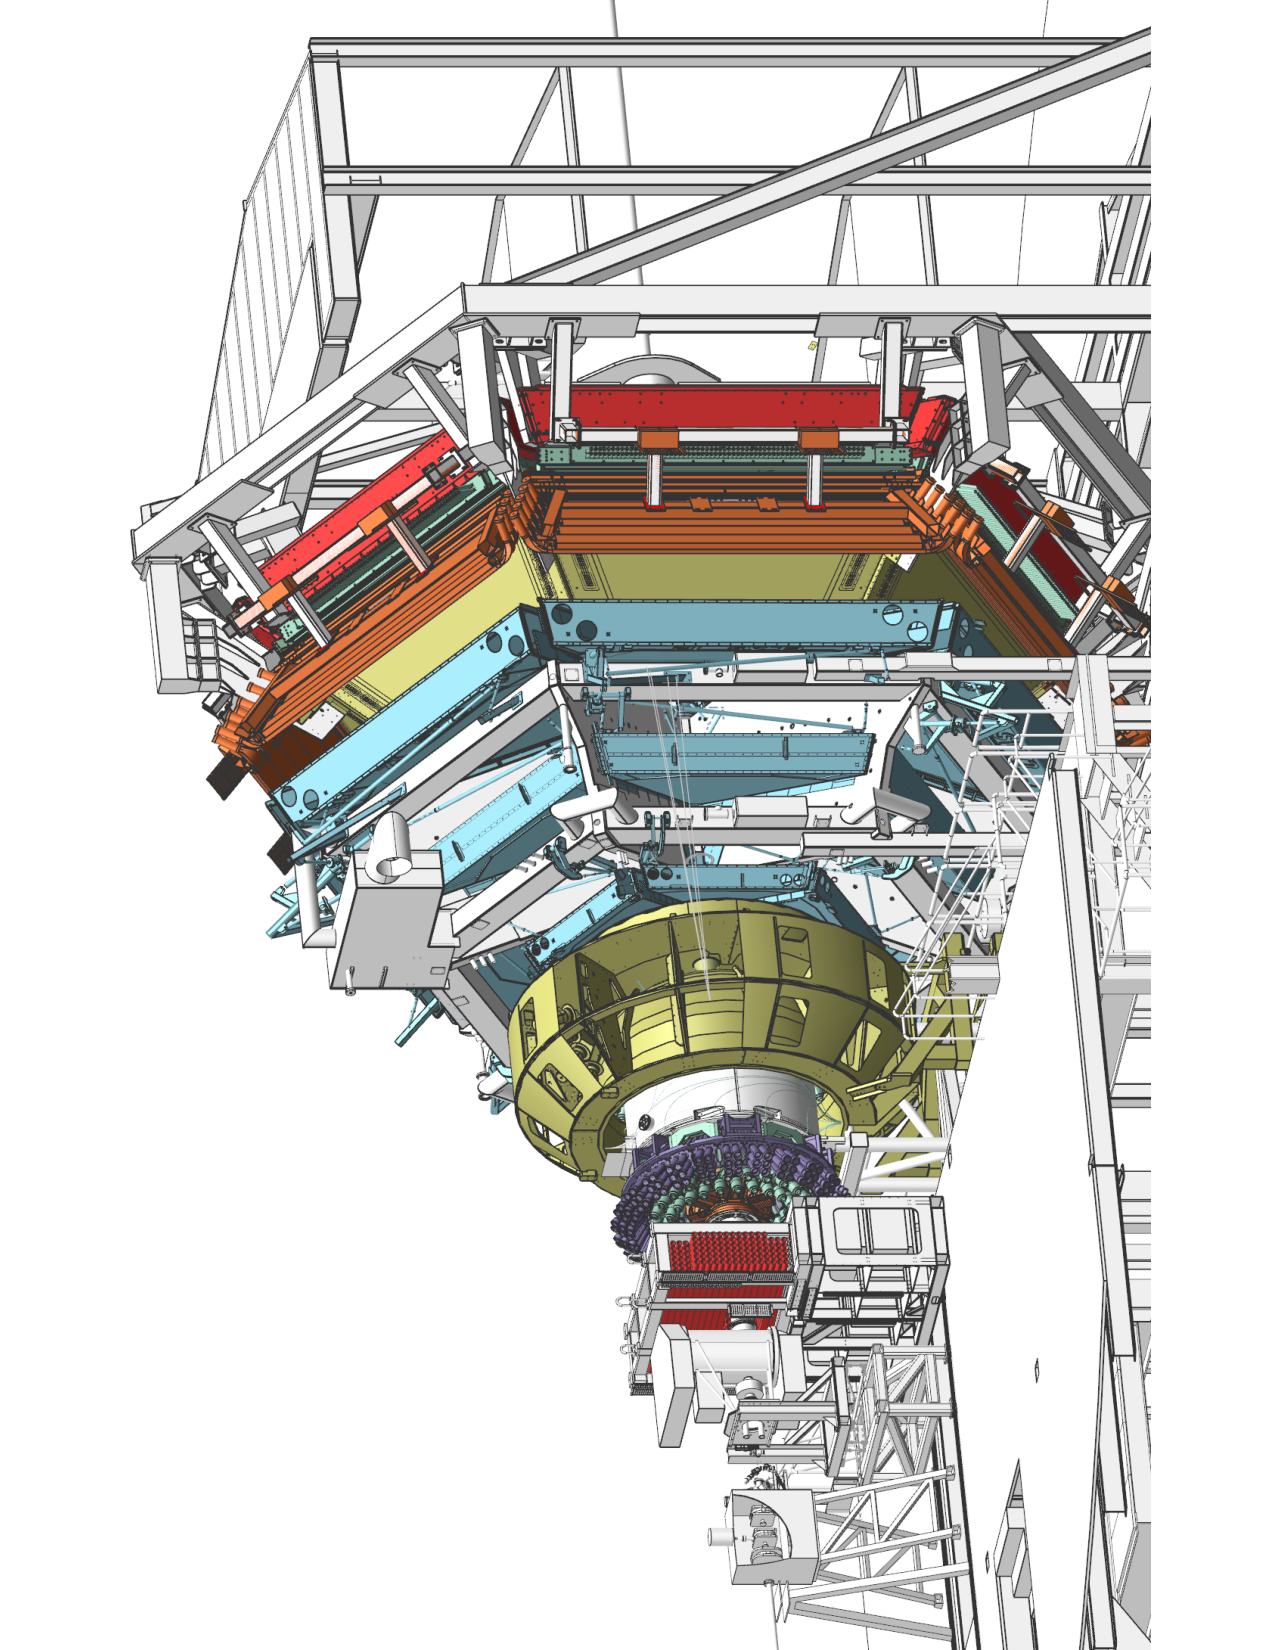
\includegraphics[width=0.35\textwidth,natwidth=610,natheight=642,angle=-90]{pics/ftof_clas12.pdf}}}
\end{picture} 
\caption{Model representation of the CLAS12 spectrometer in Hall~B at Jefferson Laboratory. The
electron beam is incident from the left side of this figure. The CLAS12 detector is roughly 20~m in
scale along the beam axis.}
\label{clas12-model}
\end{figure}
%%%%%%%%%%%%%%%%%%%%%%%%%%%%%%%%%%%%%%%%%%%%%%%%%%%%%%%%%

This paper focuses on the CLAS12 FTOF detector system and is organized as follows:
Section~\ref{clas12-fd-pid} reviews the scheme for particle identification in the CLAS12 Forward
Detector, Section~\ref{sec:overview} provides a high-level overview of the FTOF system and its
overall design requirements, Section~\ref{sec:design} provides a technical description of the system
design, and Section~\ref{sec:performance} highlights the performance of the system through both
bench testing with cosmic rays, as well as during the 2017 commissioning run and 2018 first production
running with electrons. Finally, Section~\ref{sec:summary} provides a summary of the FTOF system for
CLAS12.

\section{CLAS12 Forward Detector Particle Identification}
\label{clas12-fd-pid}

Particle identification in the CLAS12 Forward Detector relies on input from each of the different Forward
Detector subsystems. A reconstructed track in the drift chambers (DC)~\cite{dc-nim} identifies the
presence of a charged particle and is used as a veto for forward-going neutral particles. The curvature
of the particle tracks in the magnetic field of the torus provides the electric charge and momentum.
The other detector subsystems in the forward direction are used to identify the particle type. These
subsystems include the different Cherenkov counters (HTCC~\cite{htcc-nim}, LTCC~\cite{ltcc-nim}, and
RICH~\cite{rich-nim}), the electromagnetic calorimeters (ECAL)~\cite{ec-nim}, and the FTOF. These
systems are used as part of the overall CLAS12 particle identification scheme to separate the different
particle species as a function of momentum. See Ref.~\cite{clas12-nim} for details on the different
CLAS12 detector subsystems used for forward-going charged particle identification and the range of
momenta for which they are responsible for the separation of the different particle species.

The FTOF is the primary system for particle identification in CLAS12 for forward-going charged particles
for momenta up to $\sim$5~GeV. The FTOF  was designed to measure the flight time of charged particles
emerging from the target with an average time resolution of 80~ps. Given this nominal time resolution for the
counters, the momentum threshold for particle identification can be defined. For our purposes, thresholds are
given at the 4$\sigma$ level for FTOF, which amounts to the momenta where particle identification can occur
with up to an order of magnitude difference in the relative yields of the different species. The time resolution
is illustrated by computing the flight time differences between different charged particle species, pions,
kaons, and protons, for tracks normally incident on the detector. Figure~\ref{tdiff} shows the computed time
differences as a function of momentum. Where the 4$\sigma$ line crosses the computed time difference
curves defines the momentum limit for particle identification for each particle species. These limits are given
as 2.8~GeV for $\pi/K$ separation, 4.8~GeV for $K/p$ separation, and 5.4~GeV for $\pi/p$ separation.  

%%%%%%%%%%%%%%%%%%%%%%%%%%%%%%%%%%%%%%%%%%%%%%%%%%%%%%%%%
\begin{figure}[htbp]
\vspace{2.8cm}
\begin{picture}(50,50) 
\put(-2,-75)
{\hbox{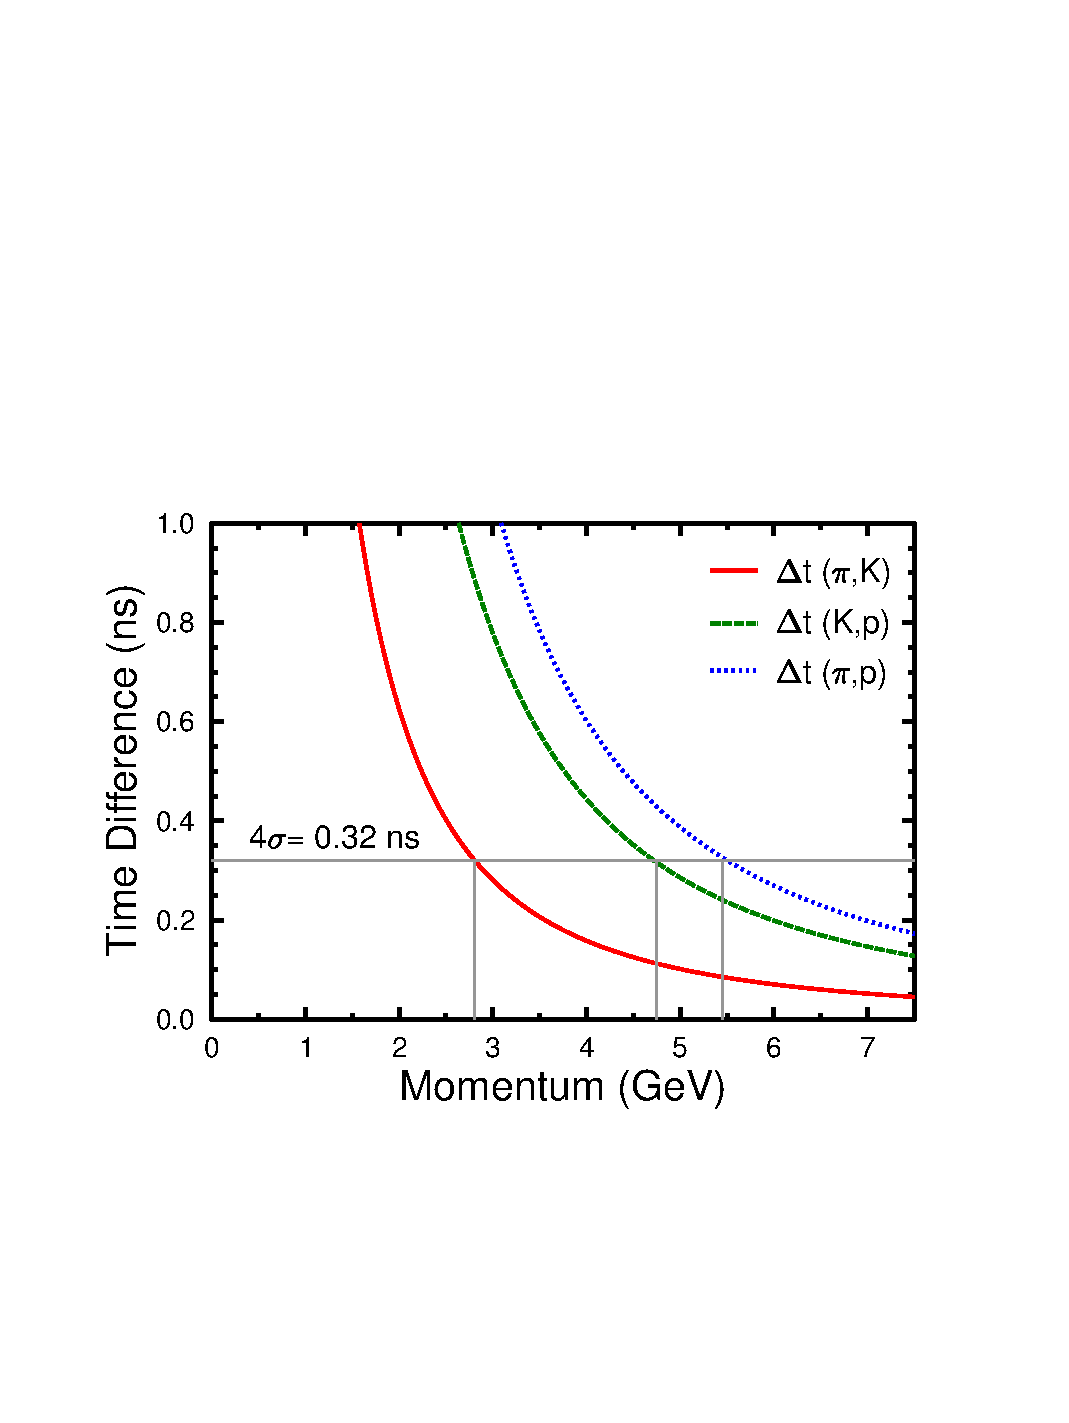
\includegraphics[width=0.6\textwidth,natwidth=610,natheight=642]{pics/tdiff_sep18.pdf}}}
\end{picture} 
\caption{Flight time differences (ns) between protons and pions, protons and kaons, and kaons and pions (as
indicated) for a 7~m path length from the target to the FTOF vs. particle momentum (GeV).  The horizontal
line indicates a time difference four times larger than the average FTOF counter design resolution of
$\sigma_{TOF} \approx$ 80~ps. The vertical lines that meet each curve represent the momentum limit for
4$\sigma$ particle species separation.}
\label{tdiff}
\end{figure}
%%%%%%%%%%%%%%%%%%%%%%%%%%%%%%%%%%%%%%%%%%%%%%%%%%%%%%%%%

Figure~\ref{pth-kin} illustrates the momentum versus polar angle coverage in CLAS12 from beam
data of a 10.6~GeV electron beam incident upon a liquid-hydrogen target. The plots show the kinematic
phase space for scattered electrons (left) and charged pions (right) for the semi-inclusive reactions
$ep \to e'\pi^{\pm}X$ ($X$ represents all other possible reaction products). For these reactions the
typical charged hadron track momenta accepted by FTOF are in the range from 0.5~GeV to 6~GeV.

%%%%%%%%%%%%%%%%%%%%%%%%%%%%%%%%%%%%%%%%%%%%%%%%%%%%%%%%%
\begin{figure}[ht]
\vspace{2.0cm}
\begin{picture}(50,50) 
\put(-5,-35)
{\hbox{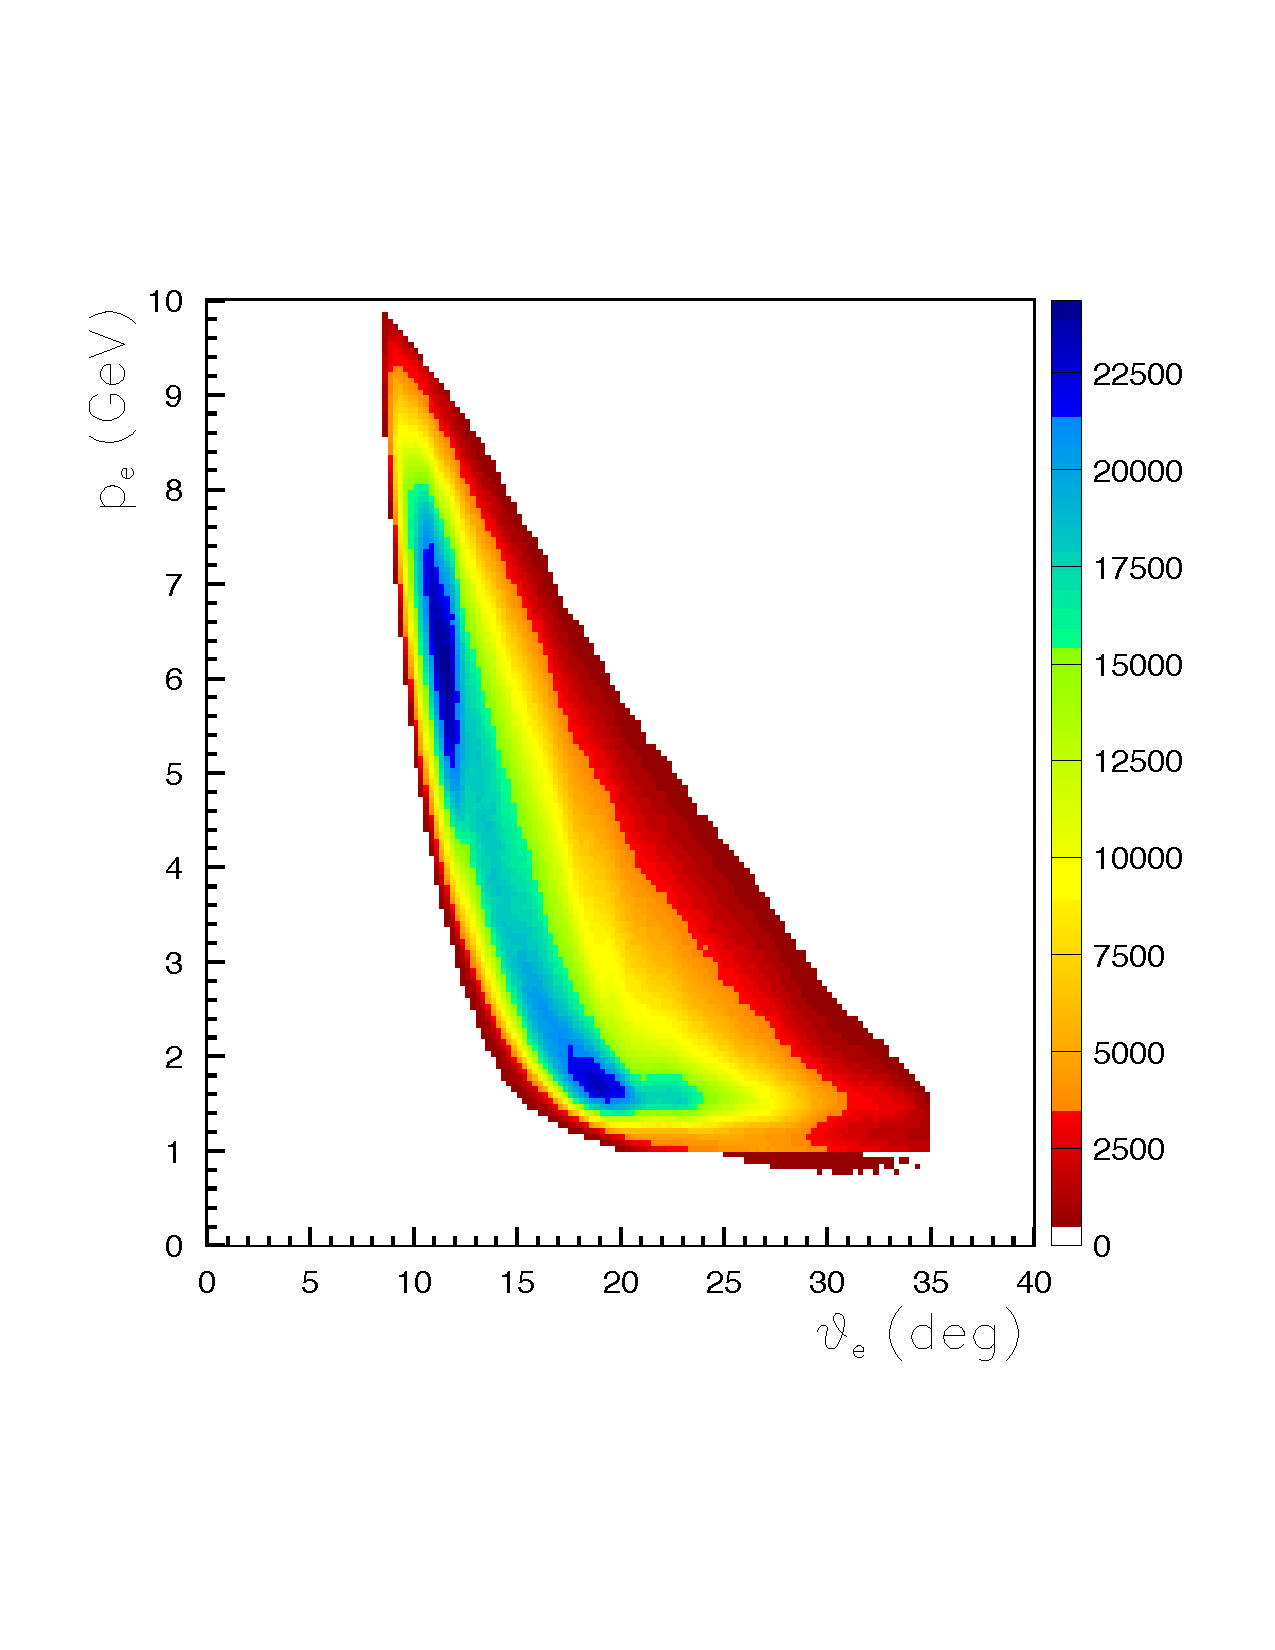
\includegraphics[width=0.27\textwidth,natwidth=610,natheight=642]{pics/pthe.pdf}}}
\put(105,-35)
{\hbox{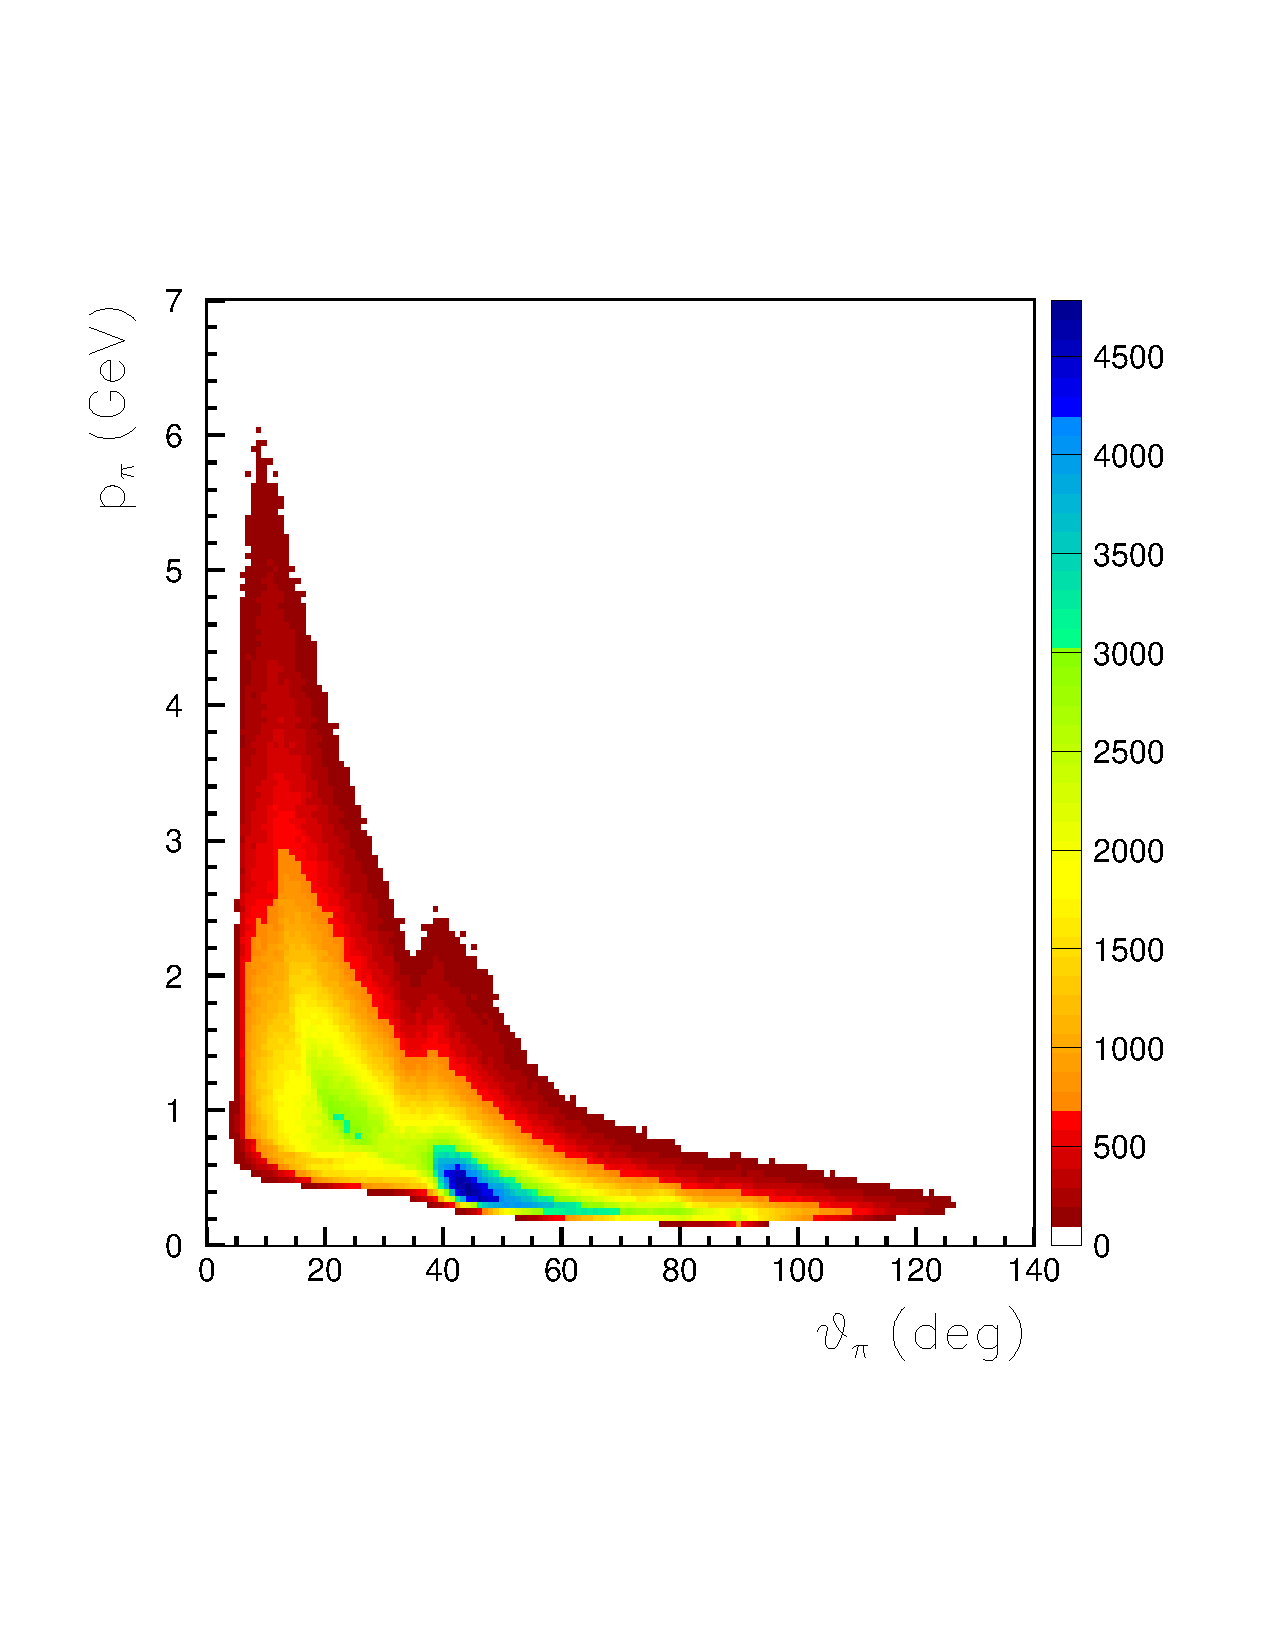
\includegraphics[width=0.27\textwidth,natwidth=610,natheight=642]{pics/pthpi.pdf}}}
\end{picture} 
\caption{Plot of momentum vs. lab polar angle from beam data for a 10.6~GeV electron beam incident
upon a liquid-hydrogen target in CLAS12 for scattered electrons (left) and $\pi^{\pm}$   (right). The
discontinuity at $\theta=35^\circ$ is due to the small acceptance gap between the Forward and Central
Detectors. The typical momentum of charged hadron tracks in the Forward Detector in these kinematics
is between 0.5~GeV and 6~GeV.}
\label{pth-kin}
\end{figure}
%%%%%%%%%%%%%%%%%%%%%%%%%%%%%%%%%%%%%%%%%%%%%%%%%%%%%%%%%

\section{Overview of the FTOF System}
\label{sec:overview}

The Forward Time-of-Flight System (FTOF) is a major component of the CLAS12 Forward Detector
used to measure the time-of-flight of charged particles emerging from interactions in the target.
The requirements for FTOF include excellent time resolution for charged particle identification and
good segmentation to minimize count rates and to provide for flexible trigger options (for details on
FTOF in the CLAS12 trigger, see Ref.~\cite{trigger-nim}). The system specifications call for an average
time resolution of $\sigma_{TOF}$=80~ps at the more forward angles of CLAS12 and 150~ps at angles
larger than 35$^\circ$. The system must also be capable of operating in a high-rate environment where
the maximum count rate for each FTOF scintillator at an operating luminosity of
$1 \times 10^{35}$~cm$^{-2}$s$^{-1}$ is up to 1~MHz.

In each of the six 60$^\circ$-wide sectors of the CLAS12 Forward Detector, the FTOF system is comprised
of three arrays of counters, referred to as panels, named panel-1a, panel-1b, and panel-2. Each panel consists
of a set of rectangular scintillators with a photomultiplier tube (PMT) on each end. Panel-1 refers to the
counters located at forward angles (5$^\circ$ to 35$^\circ$) (where two panels are employed to meet the
80~ps average time resolution requirement) and panel-2 refers to the sets of counters at larger angles
(35$^\circ$ to 45$^\circ$). The positioning and attachment of the FTOF detectors on their Forward
Carriage supports are shown in Fig.~\ref{fwd_car}.

%%%%%%%%%%%%%%%%%%%%%%%%%%%%%%%%%%%%%%%%%%%%%%%%%%%%%%%%%
\begin{figure}[htbp]
\vspace{3.9cm}
\begin{picture}(50,50) 
\put(30,-28)
{\hbox{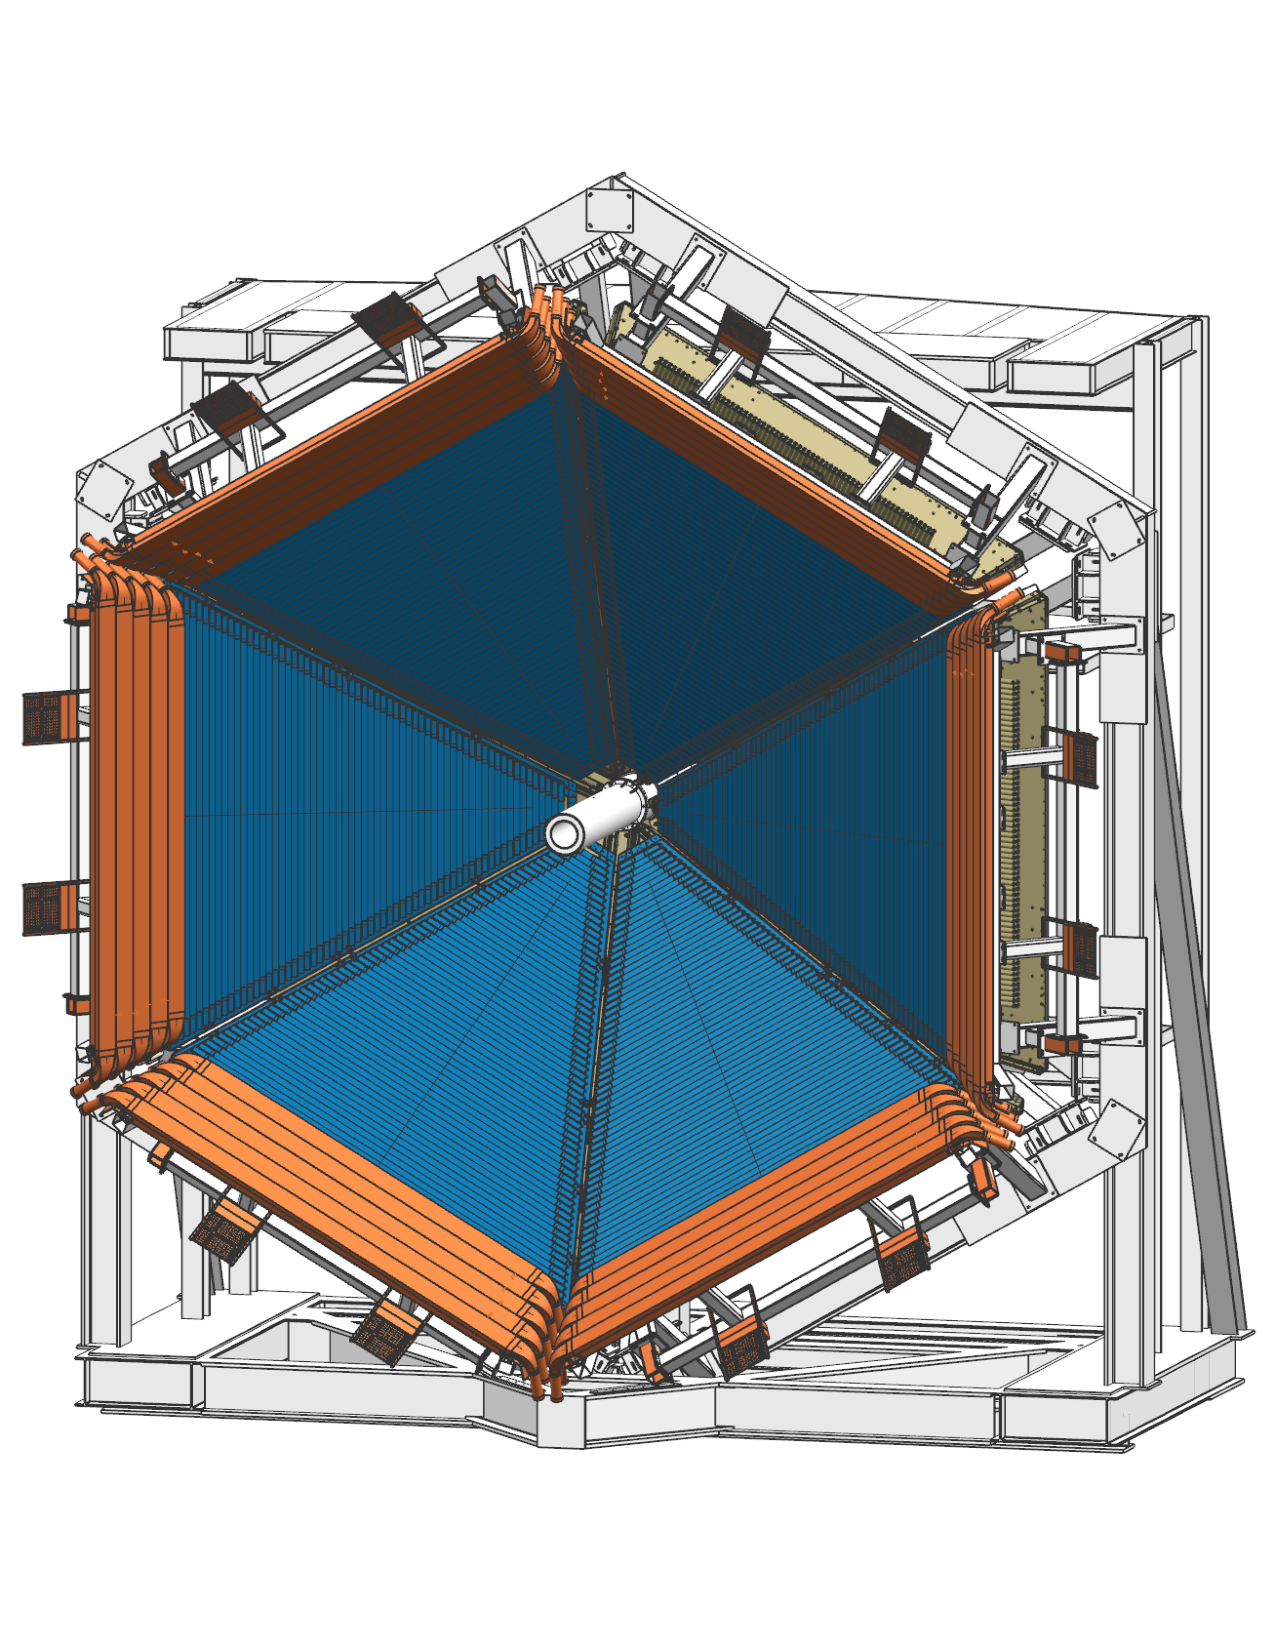
\includegraphics[width=0.35\textwidth,natwidth=610,natheight=642]{pics/fwd_carriage.pdf}}}
\end{picture} 
\caption{View of the FTOF counters for CLAS12 highlighting the location of the counters. The panel-1b
counters are shown in dark blue and the panel-2 counters, mounted around the perimeter of the Forward
Carriage, are shown in light orange. The panel-1a counters, mounted just downstream of the panel-1b
counters, are not visible in this picture. The Forward Carriage is roughly 10~m in diameter.} 
\label{fwd_car}
\end{figure}
%%%%%%%%%%%%%%%%%%%%%%%%%%%%%%%%%%%%%%%%%%%%%%%%%%%%%%%%%

The FTOF counters in the angular range from 5$^\circ$ to 35$^\circ$ consist of two sets of six 
triangular arrays. Just upstream of the electromagnetic calorimeter (ECAL) detectors, the panel-1a
arrays are mounted. These detector sets are the refurbished panel-1 TOF counters from the
decommissioned CLAS spectrometer~\cite{tof-nim}. Upstream of the panel-1a arrays the new panel-1b
arrays are mounted. In the event reconstruction the hit times for panel-1a and panel-1b are combined
together to determine the charged particle hit time (see Ref.~\cite{recon-nim} for details). In the angular
range from 35$^\circ$ to 45$^\circ$ the panel-2 arrays are mounted. These counters are refurbished
panel-2 counters of the CLAS TOF system. A detailed summary of the FTOF technical parameters is given
in Table~\ref{spec-table}. 

%%%%%%%%%%%%%%%%%%%%%%%%%%%%%%%%%%%%%%%%%%%%%%%%%%%%%%%%%
\begin{table*}[t]
\begin{center}
\begin{tabular} {c|l} \hline
~~Parameter~~ &~~~~~~~~~~~~~~~~~~~~~~ Design Value ~~~~~~~~~~\\ \hline
\multicolumn{2}{c} {Panel-1a (23 counters per sector)} \\
Angular Coverage      & $\theta = 5^\circ \to 35^\circ$, $\phi: 50\% {\rm ~at~} 5^\circ \to 85\% {\rm ~at~} 
35^\circ$ \\
Counter Dimensions   & $L = 32.3$~cm $\to$ 376.1~cm, $w \times h$ = 15~cm $\times$ 5~cm   \\
Scintillation Material & BC-408   \\
PMTs                         & EMI 9954A, Philips XP2262 \\
Counter Time Resolution     & 90~ps $\to$ 180~ps   \\ \hline
\multicolumn{2}{c} {Panel-1b (62 counters per sector)} \\
Angular Coverage      & $\theta = 5^\circ \to 35^\circ$, $\phi: 50\% {\rm ~at~} 5^\circ \to 85\% {\rm ~at~} 
35^\circ$ \\
Counter Dimensions   & $L = 17.3$~cm $\to$ 407.9~cm, $w \times h$ = 6~cm $\times$ 6~cm   \\
Scintillation Material & BC-404 (\#1 $\to$ \#31), BC-408 (\#32 $\to$ \#62)  \\
PMTs                         & Hamamatsu R9779 \\
Counter Time Resolution     & 60~ps $\to$ 110~ps   \\ \hline
\multicolumn{2}{c} {Panel-2 (5 counters per sector)} \\
Angular Coverage      & $\theta = 35^\circ \to 45^\circ$, $\phi: 85\% {\rm ~at~} 35^\circ \to 95\% {\rm ~at~} 
45^\circ$ \\
Counter Dimensions   & $L = 371.3$~cm $\to$ 426.1~cm, $w \times h$ = 22~cm $\times$ 5~cm   \\
Scintillation Material & BC-408   \\
PMTs                         & Photonis XP4312B, EMI 4312KB \\
Counter Time Resolution     & 170~ps $\to$ 180~ps   \\ \hline
\end{tabular}
\caption{Parameters for the scintillators, PMTs, and counters for the FTOF panel-1a, panel-1b, and panel-2
arrays in each of the six sectors of the CLAS12 Forward Carriage.}
\label{spec-table}
\end{center}
\end{table*}
%%%%%%%%%%%%%%%%%%%%%%%%%%%%%%%%%%%%%%%%%%%%%%%%%%%%%%%%%

The panel-1 arrays consist of the old CLAS panel-1 TOF counters (called panel-1a) and a new set of panel-1
counters (called panel-1b).  The panel-1a arrays consist of 23 scintillators, each measuring 5.08-cm thick
and 15-cm wide.  The lengths of these counters range from 32~cm at the smallest scattering angles to
376~cm at the largest scattering angles.  The scintillators are constructed from Bicron BC-408 and are
coupled to short acrylic light guides read out with 2-in Thorn EMI-9954A PMTs.  The new panel-1b arrays
consist of 62 scintillators 6-cm wide by 6-cm thick constructed from Bicron BC-404 scintillator for shortest
31 counters and BC-408 for the longest 31 counters. The lengths of these counters range from 17~cm at the
smallest scattering angles to 408~cm at the largest scattering angles. The scintillators are read out by 2-in
Hamamatsu R9779 PMTs coupled directly to the scintillation bars. These new panels are mounted to the
Forward Carriage in front of the panel-1a counter arrays. The design and bench testing results for these
counters are described in detail in Ref.~\cite{nim-p1b}.

The panel-2 arrays consist of selected counters from the old CLAS panel-2 TOF counters, and include 5
22-cm wide, 5.08-cm thick scintillators in each sector.  The length of these counters ranges from roughly
370~cm to 440~cm.  These scintillators are constructed from Bicron BC-408 and are read out through
curved acrylic light guides coupled to 3-in Philips XP4312B PMTs. These scintillators are included to give
complete acceptance for forward-going, low-momentum, outbending charged particles.  

\section{FTOF System Design}
\label{sec:design}

In order to meet the performance and mechanical requirements for the FTOF system, the major
considerations in its design included the system geometry and areal coverage, the counter time resolutions,
the system components, and the design and materials associated with its mechanical support structure in
the active area of the spectrometer. These system design elements are described in the following
subsections. In addition, this section also includes information on the readout electronics and the high
voltage system used for the FTOF.

\subsection{Geometry}
\label{ftof-geometry}

The projected space behind the coils of the CLAS12 torus as defined by straight lines projecting radially
outward from the center of the nominal target position is referred to downstream of the torus as its
``shadow'' region. This region is inactive and defines the space available for locating the light guides,
PMTs, voltage dividers, and signal and high voltage cables. The remaining area in the forward direction is
the sensitive fiducial region of the detector and must be covered by scintillation counters. The design
specification for FTOF called for a minimum of 50\% azimuthal acceptance at 5$^\circ$ increasing to
95\% at 45$^\circ$.

%%%%%%%%%%%%%%%%%%%%%%%%%%%%%%%%%%%%%%%%%%%%%%%%%%%%%%%%%
\begin{figure}[htbp]
\vspace{6.4cm}
\begin{picture}(50,50) 
\put(60,95)
{\hbox{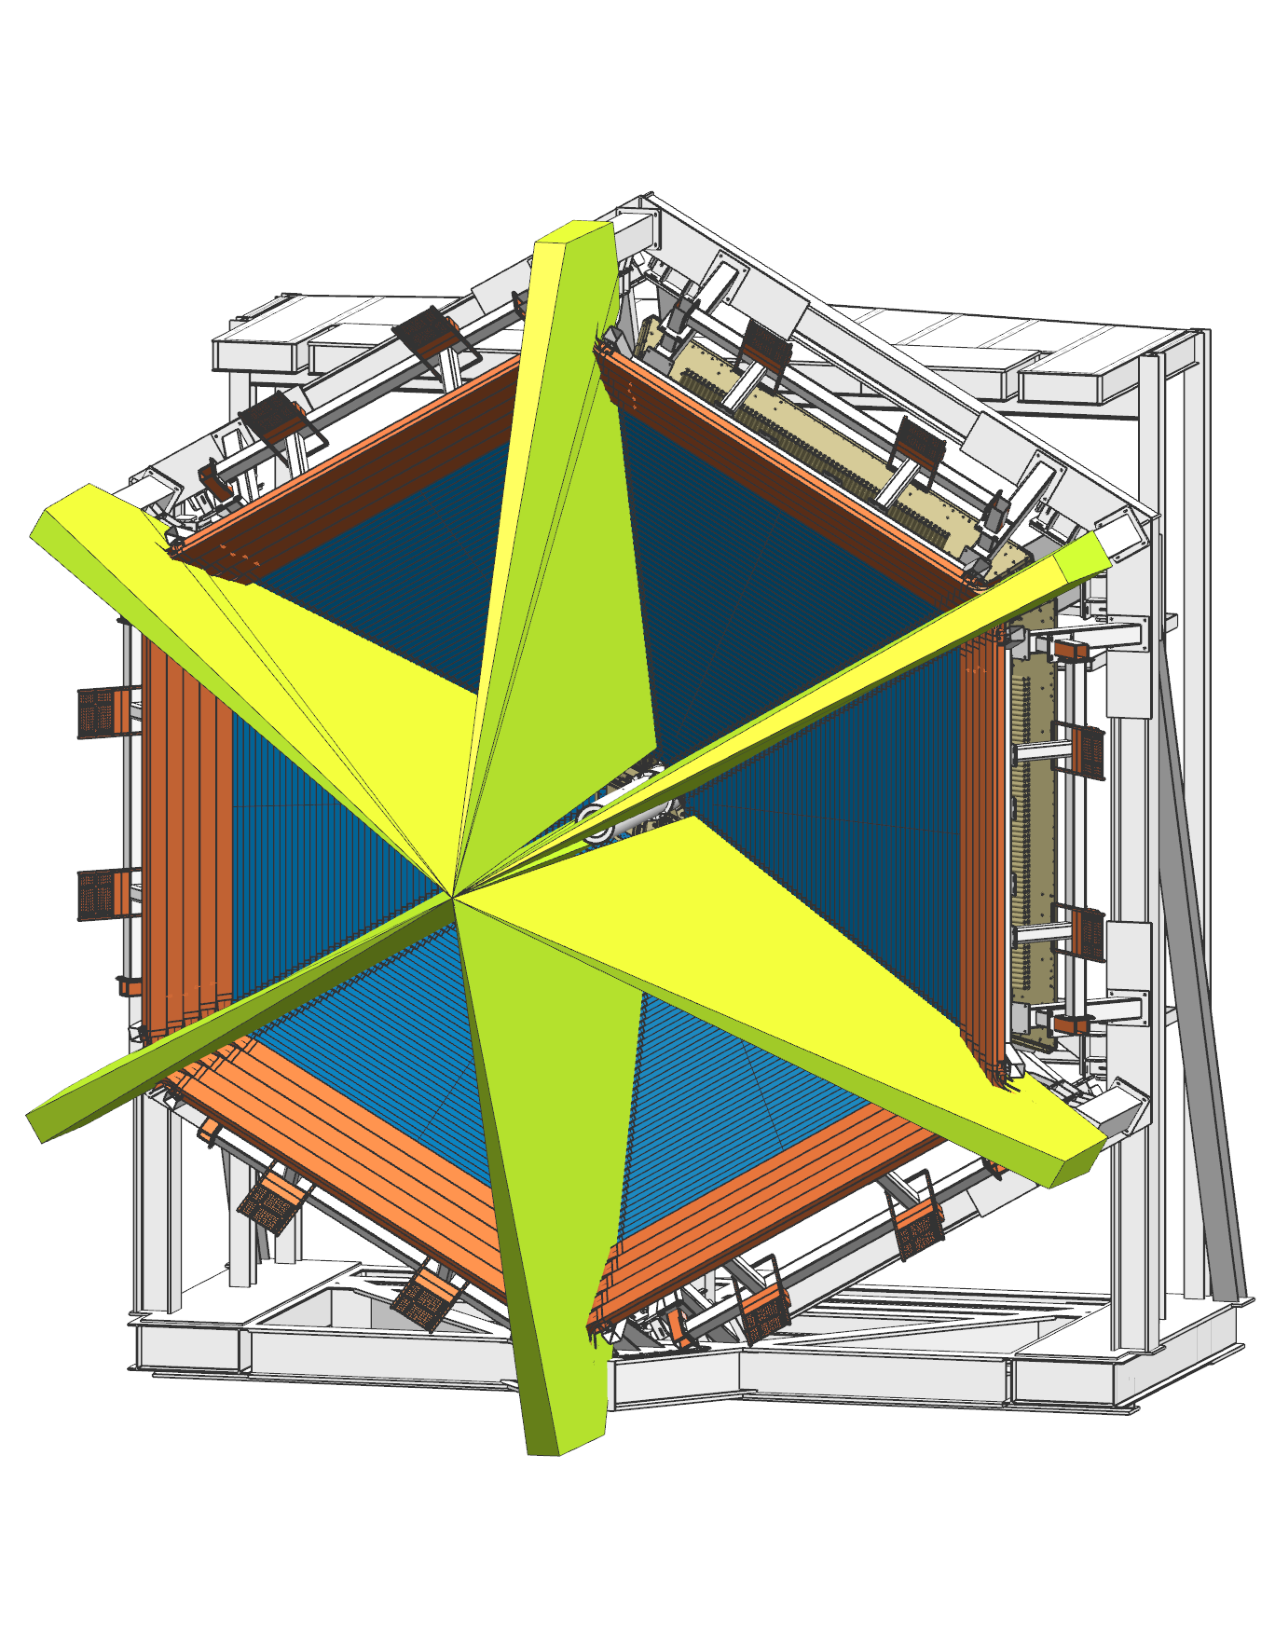
\includegraphics[width=0.26\textwidth,natwidth=610,natheight=642]{pics/fwd_shadow1.pdf}}}
\put(45,105)
{\hbox{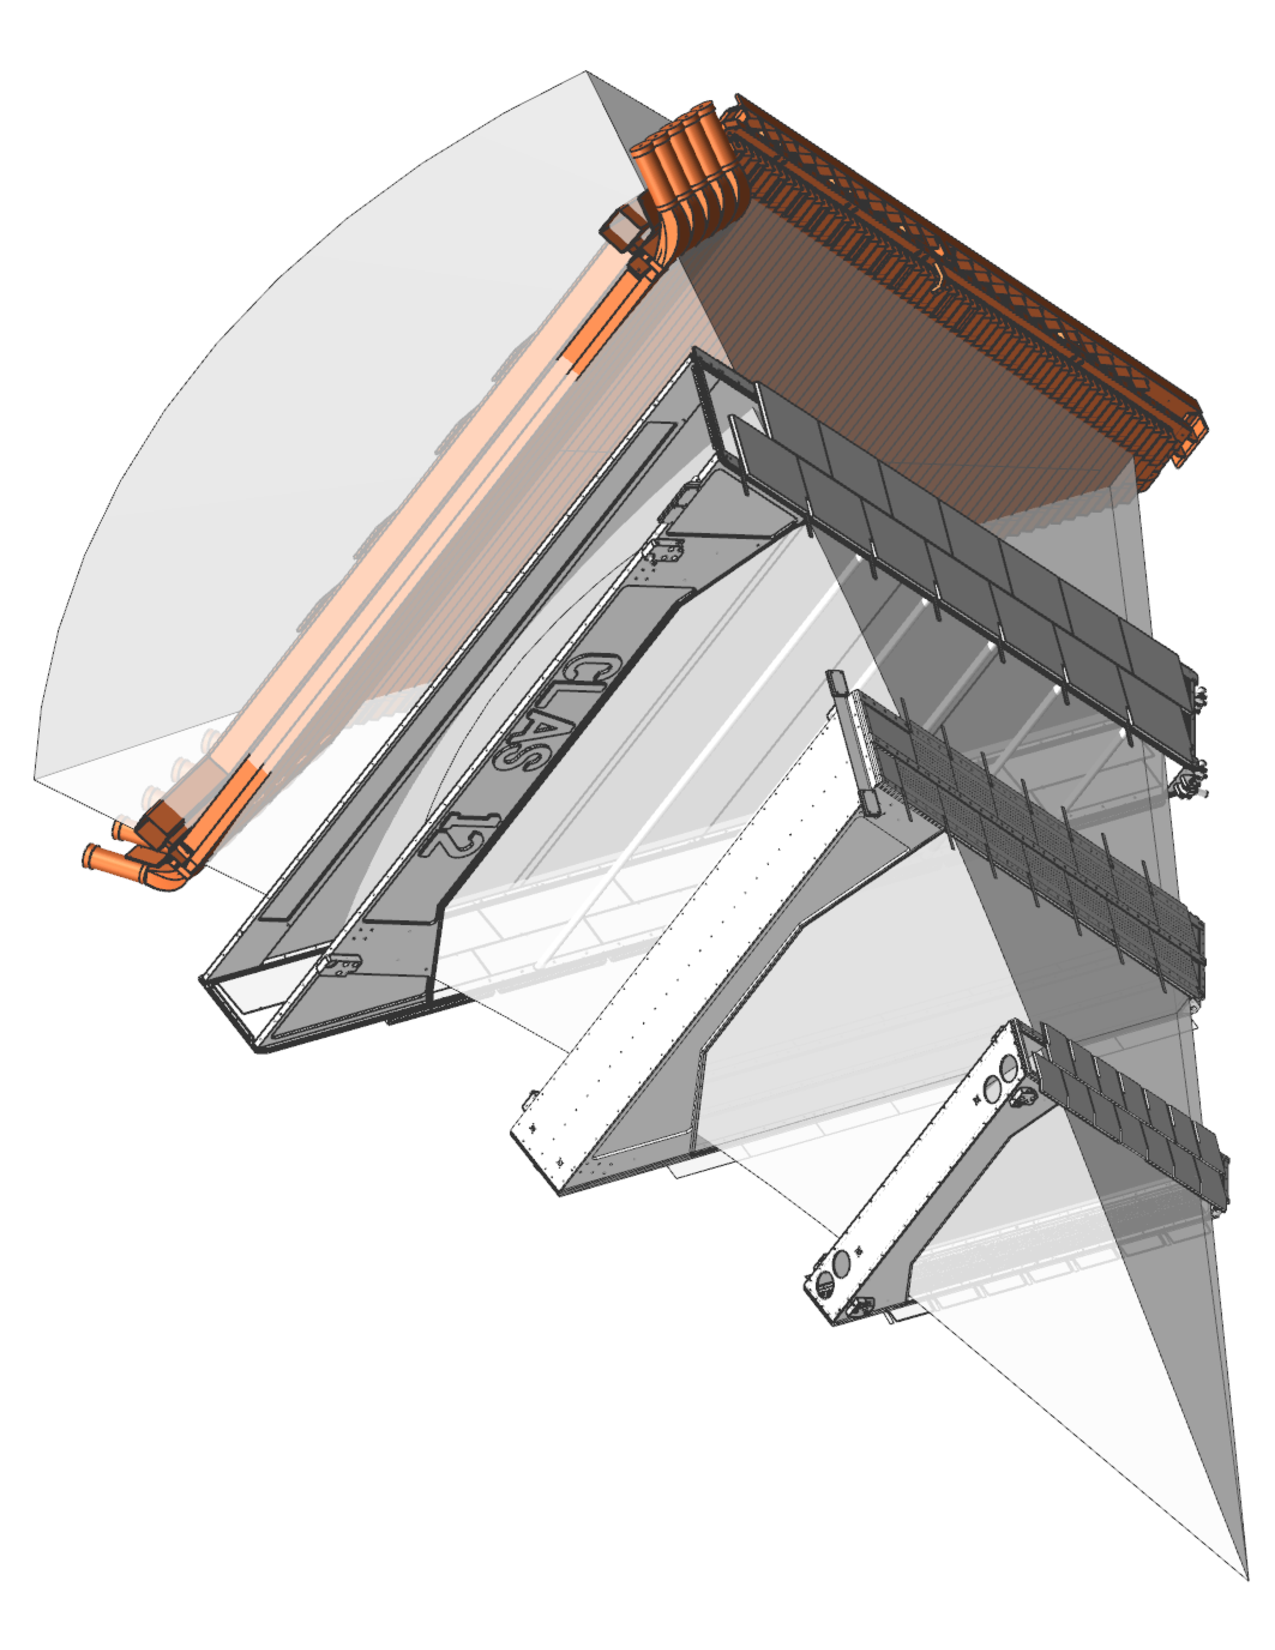
\includegraphics[width=0.24\textwidth,natwidth=610,natheight=642,angle=-90]{pics/fwd_shadow2.pdf}}}
\end{picture} 
\caption{(Top) View of the shadows created by the main torus cryostats and drift chamber endplates
as projected on the face of the FTOF system. (Bottom) The defined active area between the shadow
projections through the three regions of drift chambers projected onto the face of the FTOF in a
representative Forward Carriage sector.}
\label{shadow}
\end{figure}
%%%%%%%%%%%%%%%%%%%%%%%%%%%%%%%%%%%%%%%%%%%%%%%%%%%%%%%%%

Figure~\ref{shadow} provides an illustration of the shadow region projected onto the Forward Carriage
created primarily by the torus cryostats and the drift chamber endplates as projected onto the face of
the FTOF system. Figure~\ref{shadow}(top) shows a picture of the shadow bands on the Forward
Carriage that defines a uniform gap of $\sim$40~cm between each sector. Figure~\ref{shadow}(bottom)
shows the defined active region in one sector of CLAS12 on the face of the FTOF. The azimuthal width
of this area at the position of the Forward Carriage in Hall~B essentially defined the length of the
scintillation counters. The final limits of the shadow region at the location of FTOF are actually defined
by the endplates of the drift chamber system~\cite{dc-nim} located within the torus coils. The drift chamber
systems upstream of the torus and downstream of the torus have their endplates, on-board electronics, and
readout cables located mainly in the shadow of the torus cryostats.

The FTOF panel-1a and panel-1b arrays in each sector are triangular in shape with the shortest counters
located closest to the beamline and the longest counters furthest from the beamline. The length of each
counter for a given counter number $N_C$ is as follows:

\begin{itemize}
\item Panel-1a: \\
  $L$ [cm] = $15.85 \times N_C + 16.43$ ~~($N_C = 1 \to 5$), \\
  $L$ [cm] = $15.85 \times N_C + 11.45$ ~~($N_C = 6 \to 23$), 
\item Panel-1b: \\
  $L$ [cm] = $6.40 \times N_C + 10.84$ ~~($N_C = 1 \to 62$).
\end{itemize}

The panel-1a and panel-1b arrays are tilted toward the target at an angle of 25$^{\circ}$ consistent with
the other subsystems in the CLAS12 Forward Detector (DC, LTCC, RICH, ECAL). The panel-1a counters
are located at a radial distance from the target in the range from $R$=724.21~cm for $N_C = 1$ to
$R$=691.74~cm for $N_C = 23$. The panel-1b counters are located at a radial distance from the target
in the range from $R$=716.15~cm for $N_C = 1$ to $R$=677.97~cm for $N_C = 62$. The gap between the
coplanar panel-1b and panel-1a arrays in each sector is 10.72~cm. The minimum angle covered by panel-1a
based on a straight line from the target is 5.453$^\circ$. The corresponding minimum angle covered by
panel-1b is 3.667$^\circ$. Each of the panel-1a arrays covers an area of 7.0~m$^2$ and each of the
panel-1b arrays covers an area of 7.9~m$^2$. Figure~\ref{side-view} shows a two-dimensional schematic
of the layout and positioning of the arrays defining the key geometry parameters, which are listed in
Table~\ref{geom-parms}. See Ref.~\cite{ftof-geom} for more information.

The panel-2 arrays are mounted outside of the panel-1a and panel-1b arrays at larger polar angles as shown
in Fig.~\ref{side-view}. The length of each counter for a given counter number $N_C$ is as follows:

\begin{itemize}
\item Panel-2: \\
  $L$ [cm] = $13.73 \times N_C + 357.55$~~ ~~($N_C = 1 \to 5$).
\end{itemize}

The panel-2 arrays are tilted toward the target at an angle of 58.11$^\circ$. The minimum angle covered
by panel-2 based on a straight line from the target is 34.698$^\circ$. Each of the six panel-2 arrays covers
an area of 4.4~m$^2$. Note that the panel-2 arrays have no direct line of sight to the target due to the
solenoid. However, due to the presence of the toroidal magnetic field, they provide additional acceptance for
outbending, low momentum tracks  and for tracks associated with strange particles that decay in-flight after
emerging from the target (e.g. $\Lambda \to N \pi$ with $c \tau = 7.89$~cm).

%%%%%%%%%%%%%%%%%%%%%%%%%%%%%%%%%%%%%%%%%%%%%%%%%%%%%%%%%
\begin{figure}[htbp]
\vspace{2.2cm}
\begin{picture}(50,50) 
\put(0,-33)
{\hbox{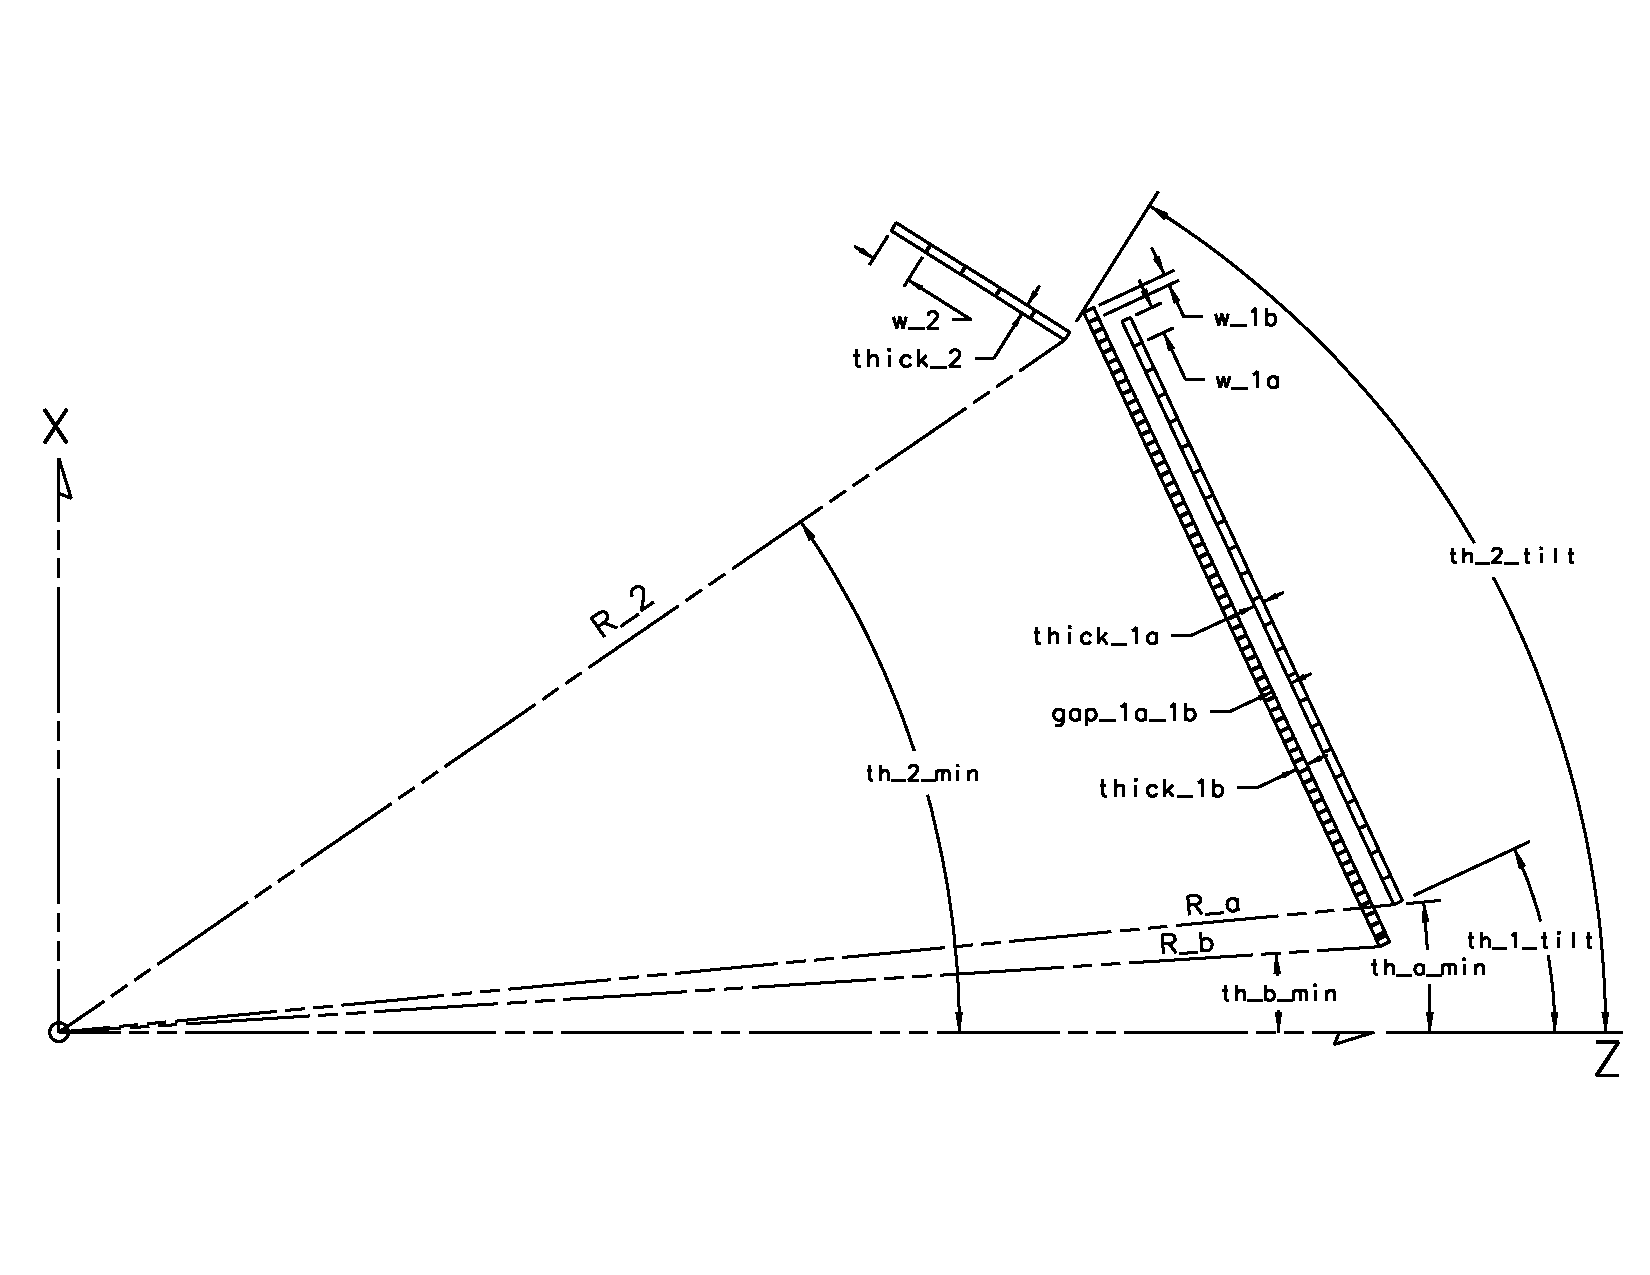
\includegraphics[width=0.36\textwidth,natwidth=610,natheight=642]{pics/side-view.pdf}}}
\end{picture} 
\caption{View of the FTOF scintillators for panel-1a, panel-1b, and panel-2 in the sector mid-plane for one
representative sector of the CLAS12 Forward Detector with the key parameters indicated.}
\label{side-view}
\end{figure}
%%%%%%%%%%%%%%%%%%%%%%%%%%%%%%%%%%%%%%%%%%%%%%%%%%%%%%%%%

%%%%%%%%%%%%%%%%%%%%%%%%%%%%%%%%%%%%%%%%%%%%%%%%%%%%%%%%%
\begin{table*}[htbp]
\begin{center}
\begin{tabular} {c|c|c|c} \hline
Parameter & Panel-1a &  Panel-1b & Panel-2 \\ \hline
R\_min      & 726.689~cm & 717.236~cm & 659.71~cm \\
th\_min    & 5.453$^\circ$ & 3.667$^\circ$ & 34.698$^\circ$ \\
th\_tilt    & 25.00$^\circ$ & 25.00$^\circ$ & 58.11$^\circ$ \\
thick        & 5.08~cm           & 6.00~cm         & 5.08~cm \\ 
width       & 15.00~cm         & 6.00~cm         & 22.00~cm \\
gap\_1a\_1b & \multicolumn{2}{c|}{10.717~cm} &  -- \\ \hline
\end{tabular}
\caption{Nominal geometry parameters for the CLAS12 FTOF detector system.}
\label{geom-parms}
\end{center}
\end{table*}
%%%%%%%%%%%%%%%%%%%%%%%%%%%%%%%%%%%%%%%%%%%%%%%%%%%%%%%%%%

Given the active area coverage requirements for the FTOF system within each CLAS12 sector on the
Forward Carriage, another key aspect of the geometry associated with the FTOF system design is
the width of the individual scintillation counters. An essential optimization was made to select the
counter width to minimize the number of readout channels, while considering the overall count rates per
bar at the nominal luminosity associated with incident charged and neutral particles (including photons).
These rates must allow for reasonable PMT anode currents that do not affect the stability of the PMT
response in terms of pulse shape or saturation effects, nor lead to unreasonably short PMT lifetimes.
In addition, the width of the scintillation bars determines the granularity of the scattering angle definition
in the trigger and its matching to the projected tracks from the drift chambers to the electromagnetic
calorimeters. Note that the 15-cm widths of panel-1a and the 22-cm widths of panel-2 of the existing
refurbished counters of the CLAS TOF system were optimized for nominal beam-target luminosities a
factor of 10 lower than for CLAS12. The 6-cm widths of the newly constructed panel-1b counters were
optimized for the higher rate operating conditions of CLAS12.

\subsection{Counter Hit Time Resolution}
\label{res-sec}

The FTOF counters are designed to provide an output signal for the CLAS12 data acquisition system
\cite{daq-nim} that reflects the time a charged particle passed through the scintillation counter. As the
particle passes through the scintillation material, it causes ionization that subsequently generates
scintillation light. The photons that are created travel on various paths inside of the scintillator and light
guide (if present), and may get absorbed or reflected (internally or on outer wrapping materials) before
they can impinge on the photocathode of the PMT. This interaction produces a photoelectron signal that is
amplified within the stages of the PMT and the generated pulse is then input into the readout electronics,
which includes an analog-to-digital converter (ADC), a discriminator, and a time-to-digital converter (TDC)
(see Section~\ref{sec-elec} for details). The net effect of these different processes accounts for the time
resolution of the counter.

The contributions to the time resolution of time-of-flight systems have been parameterized in
Ref.~\cite{kuhlen} by:

\begin{equation}
\label{timing-func}
\sigma_{TOF} = \sqrt{\sigma_0^2 + \frac{\sigma_1^2 + (\sigma_2 L/2)^2} {N_{pe}}}.
\end{equation}

\noindent
Here $\sigma_{TOF}$ represents the timing resolution for a scintillation counter with double-sided PMT
readout. $\sigma_0$ represents the intrinsic electronic resolution of the measurement system, a
floor-term contribution that is independent of the light level. The remaining terms $\sigma_1$ and
$\sigma_2$ are directly dependent on the average photo-statistics seen at either of the PMT
photocathodes $N_{pe}$ (see Eq.(\ref{nphe-eq})). The term $\sigma_1$ models the jitter in the combined
single photoelectron response of the scintillation counter and its PMTs and the term $\sigma_2$ accounts
for path length variations in the light collection.  These path length variations in the scintillator scale with
the distance from the source to the PMT, which we take to be half the length of the counter ($L/2$), since
the scintillators are read out at either side.  The statistical behavior of the last two terms is indicated by
scaling the single-photoelectron responses by $\sqrt{N_{pe}}$. For scintillators that are several meters
long, the dominant contribution to the timing resolution comes from transit time variations of photon paths
along the scintillator to the PMT due to the counter geometry.

The values of the parameters $\sigma_0$, $\sigma_1$, and $\sigma_2$ for the panel-1a and panel-2
counters are given in Ref.~\cite{tof-nim}, where the above functional form with the parameters listed
in Table~\ref{timing-parms} was found to describe the measured data. A direct extension of these
parameters is assumed to be reasonable for estimating the time resolution for the panel-1b counters.
A summary of all parameters employed are listed in Table~\ref{timing-parms}. Note that due to
improvements in the resolution of the readout electronics for the CLAS12 FTOF system compared to
the CLAS TOF system, the floor-term $\sigma_0$ has been reduced from 62~ps to 40~ps. 

%%%%%%%%%%%%%%%%%%%%%%%%%%%%%%%%%%%%%%%%%%%%%%%%%%%%%%%%%
\begin{table*}[htbp]
\begin{center}
\begin{tabular} {c|c} \hline
Parameter    & Nominal Value\\ \hline
$\sigma_0$ & 0.062~ns (CLAS TOF); 0.040~ns (CLAS12 FTOF) \\ 
$\sigma_1$  & 2.1~ns (panel-1a/1b); 2.0~ns (panel-2) \\ 
$\sigma_2$  & 2.0~ns/m \\ 
$N_{pe}^0$   & 918 \\
$\lambda$   & $0.358\cdot L + 81.725$~cm \\ \hline
\end{tabular}
\caption{Parameters determined for the CLAS TOF panel-1a and panel-2 counters in Ref.~\cite{tof-nim}
and used for a parameterization of the CLAS12 FTOF counters using the functional form for $\sigma_{TOF}$
in Eq.(\ref{timing-func}) and for $N_{pe}$ in Eq.(\ref{nphe-eq}).}
\label{timing-parms}
\end{center}
\end{table*}
%%%%%%%%%%%%%%%%%%%%%%%%%%%%%%%%%%%%%%%%%%%%%%%%%%%%%%%%%%

The number of photoelectrons $N_{pe}$ in Eq.(\ref{timing-func}) for panel-1a and panel-2 at the PMT
photocathode was determined in Ref.~\cite{tof-nim} by:

\begin{equation}
\label{nphe-eq}
N_{pe} = N_{pe}^0 {\rm exp} \left( \frac{L_0}{2 \lambda_0} - \frac{L}{2 \lambda} \right) \cdot F,
\end{equation}

\noindent
where $N_{pe}$ for all counters was referenced to the average value measured for the response of
the shortest panel-1a counter $N_{pe}^0$ of length $L_0=32$~cm with attenuation length $\lambda_0$.
The attenuation length of the scintillation bars represents the distance $\lambda$ into the material
where the probability that the photon has been absorbed is $1/e$. For the panel-2 counters, $N_{pe}$
is further scaled by the factor $F = 0.9$ to account for light collection efficiencies at the end of the
larger panel-2 counters with their 3-in PMTs and longer light guides compared to the smaller panel-1a
PMTs with their relatively short light guides~\cite{tof-nim}. For the panel-1b counters, $N_{pe}$ is
determined as for panel-1a using Eq.(\ref{nphe-eq}) by scaling by the ratio of the cross sectional areas
of the scintillation bars (15~cm $\times$ 5~cm vs. 6~cm $\times$ 6~cm). 

Figure~\ref{sigma_tof} shows the parameterized resolution for the counters in panel-1a, panel-1b,
and panel-2 as a function of counter length. The Forward Detector event reconstruction and particle
identification uses time information from both panel-1a and panel-1b. For tracks that pass through both
arrays the combined time information (described in Ref.~\cite{recon-nim}) is used and results in a 20\%
improvement compared to using the hit information from panel-1b alone.

%%%%%%%%%%%%%%%%%%%%%%%%%%%%%%%%%%%%%%%%%%%%%%%%%%%%%%%%%
\begin{figure}[htbp]
\vspace{2.4cm}
\begin{picture}(50,50) 
\put(-5,-45)
{\hbox{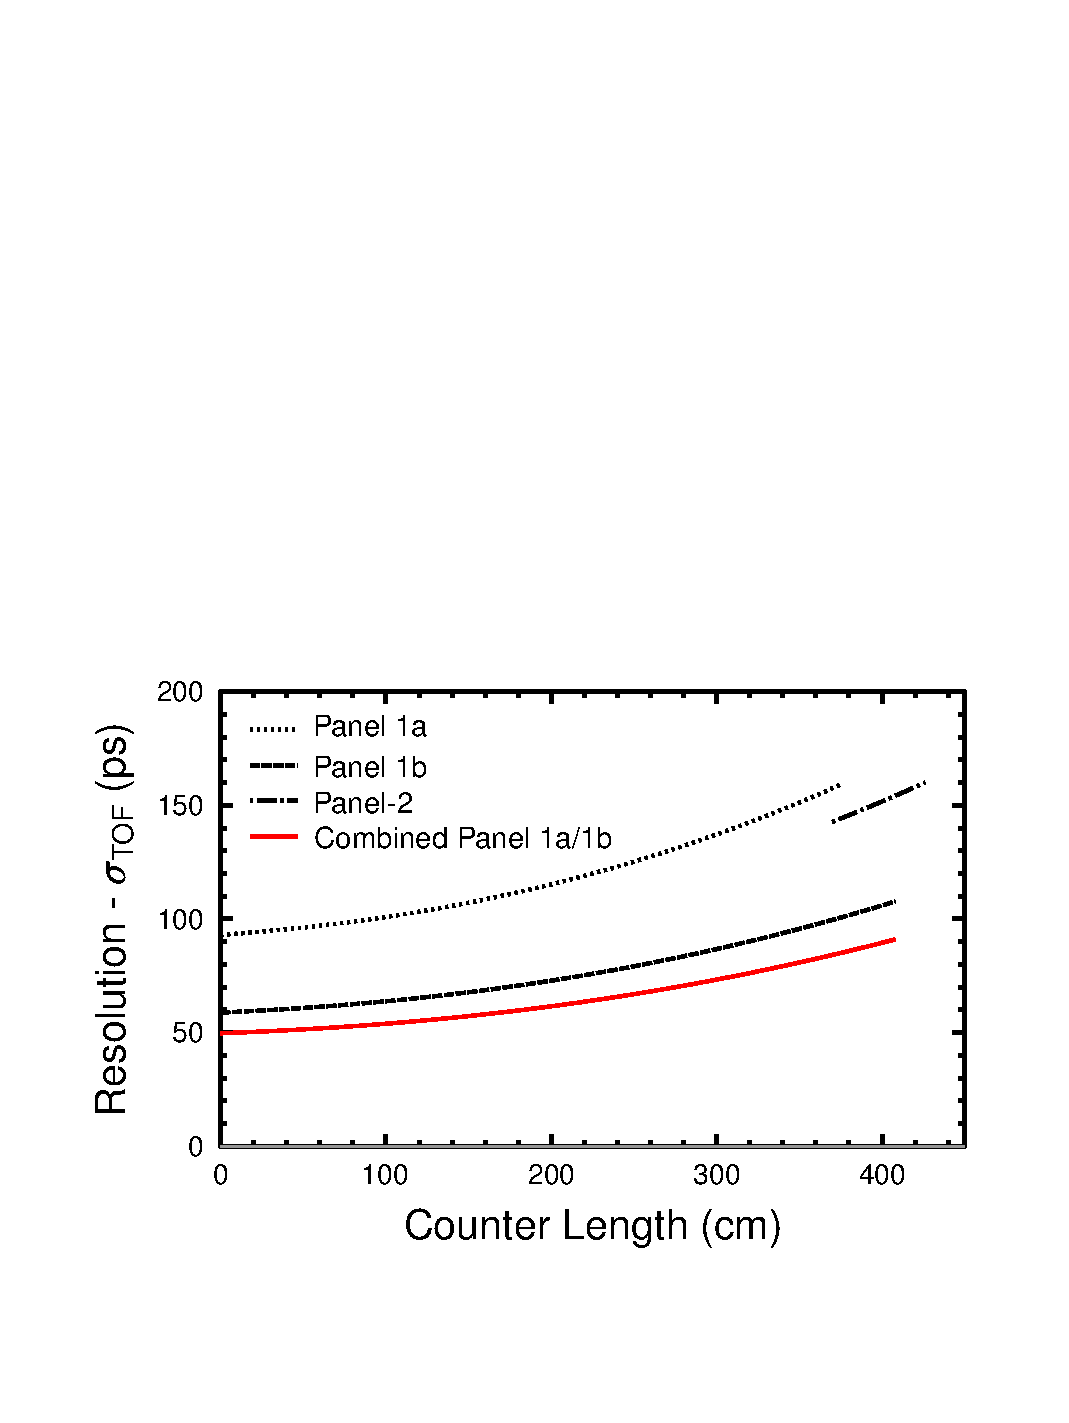
\includegraphics[width=0.6\textwidth,natwidth=610,natheight=642]{pics/resolution.pdf}}}
\end{picture} 
\caption{Parameterized expectation of the counter hit time resolution for the FTOF panel-1a (dotted),
panel-1b (dashed), and panel-2 (dot-dashed) counters as a function of length. The solid (red) line
indicates the final expected resolution in the forward direction by combining the hit time information
from the panel-1a and panel-1b counters. The horizontal line indicates the 80~ps average time resolution
specification for the FTOF system.}
\label{sigma_tof}
\end{figure}
%%%%%%%%%%%%%%%%%%%%%%%%%%%%%%%%%%%%%%%%%%%%%%%%%%%%%%%%%

\subsection{System Components}

\subsubsection{Scintillator Material}

To optimize the time resolution over the full volume of the FTOF counters, scintillation materials with
fast time response and long attenuation length are essential. For the panel-1a and panel-2 FTOF counters
that were refurbished from the older CLAS TOF system, Bicron BC-408 was selected. For the panel-1b
counters constructed for the new CLAS12 FTOF system, a different design approach was considered
that optimized the overall system time resolution. For counters less than 2~m in length, the overall
performance is improved by the use of a faster scintillator with a small decay time $\tau_{decay}$, whereas
for the longer counters, a material with a longer attenuation length is the better choice. The final decision
for the panel-1b counters was to use BC-404 for counters 1 $\to$ 31 (lengths from 17.3~cm to 209.4~cm)
and BC-408 for counters 32 $\to$ 62 (lengths from 215.8~cm to 407.9~cm). Table~\ref{scint-specs}
lists the properties of the FTOF scintillation materials.

%%%%%%%%%%%%%%%%%%%%%%%%%%%%%%%%%%%%%%%%%%%%%%%%%%%%%%%%%
\begin{table*}[t]
\begin{center}
\begin{tabular}{c|c|c} \hline
Property                                    & BC-404     & BC-408  \\    
Light Output, \% Anthracene  & 68             &  64    \\ 
Rise Time (ns)                           & 0.7             & 0.9    \\ 
Decay Time (ns)                         & 1.8             & 2.1     \\ 
Pulse Width, FWHM (ns)         & 2.2              & 2.5    \\ 
Wavelength of maximum emission (nm) & 408    & 425 \\ 
Light attenuation length (cm)   & 140             & 210   \\ 
Bulk attenuation length (cm)     & 160             & 380  \\ 
Polymer base                             & \multicolumn{2}{c}{Polyvinyltoluene} \\ 
Refractive index                       & \multicolumn{2}{c}{1.58}                    \\  
Density (g/cm$^3$)                  & \multicolumn{2}{c}{1.023}                    \\ \hline 
\end{tabular}
\end{center}
\caption{Properties of the plastic scintillation material BC-404 and BC-408 employed for the counters
of the FTOF system~\cite{scint-mat-ref}.}
\label{scint-specs}
\end{table*}
%%%%%%%%%%%%%%%%%%%%%%%%%%%%%%%%%%%%%%%%%%%%%%%%%%%%%%%%%

The bulk attenuation length of the scintillation material is stated by its manufacturer to be 160~cm
for BC-404 and 380~cm for BC-408. However, the practical attenuation length of the prepared bars
is smaller than the nominal bulk value as the actual path length of photons from the charged particle
intersection point to the ends of the bar is increased and reflections occur due to the finite geometry
of the bar. For optimal response, this practical attenuation length should typically be longer than the
bar to ensure sufficient photon statistics. Measurements of the practical attenuation length of the
FTOF counters are given in Section~\ref{sec:attlen}.

\subsubsection{Photomultiplier Tubes and Voltage Dividers}

The panel-1a counters are read out at either end through 2-in diameter Thorn EMI 9954A PMTs (later
manufactured by ElectronTubes). The PMTs are coupled to the scintillation bars using 12-cm-long acrylic
light guides that match the 15~cm $\times$ 5~cm scintillator on one end and the 2-in diameter PMT on
the other end.  For the panel-2 counters, 3-in diameter Philips XP4312B/D1 3-in PMTs (later manufactured
by Photonis) are employed. The PMTs are coupled to the scintillators through acrylic light guides that match
the 22~cm $\times$ 5~cm scintillator on one end and the 3-in diameter PMT on the other end. Both the
9954A and XP4312B/D1 PMTs have 12 linear-focused dynode stages. For both the panel-1a and panel-2
counters the PMTs are glued on the light guides using BC-600 optical glue. See Ref.~\cite{tof-nim} for
full details on the PMT selection criteria and the light guide designs.

The voltage dividers employed for the panel-1a and panel-2 readout are custom units built specifically
for the CLAS TOF project~\cite{tof-nim}. The dividers use high voltage field-effect transistors to fix
the PMT gain by stabilizing the voltage and to protect the PMT against high light levels by shutting down
the circuit in case of over-current. The grid voltage for both types of dividers followed the
manufacturer's specifications.

The photomultipliers employed for the panel-1b counters are 2-in diameter Hamamatsu R9779 PMTs with
a high gain selection (minimum $0.5 \times 10^5$, average $1.0 \times 10^6$) that have been integrated
with a voltage divider to form the R9779-20MOD assembly. These PMTs include 8 linear-focused dynode
stages. This high time resolution PMT was selected due to its particularly compact overall assembly length
of 113~mm. The length restriction was necessary to fit within the defined shadow region of the torus
cryostats at the location of the PMTs (see Section~\ref{ftof-geometry} for details). These PMTs are
coupled directly to the ends of the scintillation bars using BC-600 optical glue. The performance
specifications for all FTOF PMTs are listed in Table~\ref{pmt-specs}.

%%%%%%%%%%%%%%%%%%%%%%%%%%%%%%%%%%%%%%%%%%%%%%%%%%%%%%%%%
\begin{table*}[htbp]
\begin{center}
\begin{tabular}{c|c|c|c} \hline
                                                           & 9954A                    & R9779                     & XP4312B/D1 \\ \hline
Property                                            & Panel-1a                   & Panel-1b                  & Panel-2 \\
Diameter                                           & 2~in                         & 2~in                        & 3~in \\ 
Photocathode area                            & 16.6~cm$^2$           & 16.6~cm$^2$        & 36.3~cm$^2$ \\ 
Dynode stages                                  & 12                            & 8                              & 12 \\
Spectral response                            & 290 $\to$ 680~nm & 300 $\to$ 650~nm & 290 $\to$ 650~nm \\ 
Max. wavelength emission               & 400~nm & 420~nm & 420~nm \\ 
Gain                                                    & 1.8$\times$10$^7$ & 5.0$\times$10$^5$ & 3$\times$10$^7$ \\ 
Quantum eff. @ $\lambda_{max}$   & 28\% & 28\% & 28\% \\ 
Max. anode current rating               & 100~$\mu$A & 100~$\mu$A & 100~$\mu$A \\ 
Anode dark current                         & 2~nA & 10~nA & 10~nA \\ 
Anode pulse rise time                      & 2~ns & 1.8 ns & 2.1 ns \\ 
Electron transit time                        & 41 ns & 20 ns & 31 ns \\
Transition time spread                     & 0.4~ns & 0.25 ns & 0.4 ns \\ \hline
\end{tabular}
\end{center}
\caption{Properties of the PMTs used for the readout of the FTOF panel-1a, panel-1b, and panel-2
counters. All of these PMTs have a borosilicate glass window and employ green-sensitive bialkali
photocathodes.}
\label{pmt-specs}
\end{table*}
%%%%%%%%%%%%%%%%%%%%%%%%%%%%%%%%%%%%%%%%%%%%%%%%%%%%%%%%%

\subsubsection{PMT Magnetic Shielding}

The FTOF PMTs are located in the range from 6.2~m to 7.2~m from the target in a region where the
stray magnetic field from the torus is computed to be less than 30~G when the torus is operated at full
field. Custom magnetic shields for the PMTs are included to reduce both the axial and transverse
components of the field along the full accelerating structure of the PMT to a level of less than 0.2~G.
For the panel-1a counters, the PMT magnetic shields consist of 7.5-in long, 2-in diameter, 0.040-in thick
$\mu$-metal cylinders. For the panel-2 counters, the PMT magnetic shields consist of a 9.5-in long, 3-in
diameter, 1.5-mm thick $\mu$-metal cylinders. These shields extend from the voltage divider attachment
point to 2~in beyond the front face of the PMT. They are held in place by the PMT itself and the counter
support structure (see Ref.~\cite{tof-nim} for details).  For the panel-1b counters, the magnetic shields
are composed of 2-mm thick $\mu$-metal boxes, 6.7-in long by 2.36-in wide. These boxes contain the
entire voltage divider assembly and extend 1.6~in beyond the front face of the PMT. Note that the last
4~cm of each end of the panel-1b scintillation bars were machined down to a width of 5.6~mm (with a
diamond-tool finish) to allow the shield boxes to fit over the ends of the bars. The shields are screwed
down to the counter support structure to hold them into position. The face of the shield box opposite the
PMT side has a small penetration to allow the signal and HV cables and connectors to pass through. Further
details on the FTOF magnetic shielding and the field tests that were conducted are included in
Ref.~\cite{ftof-shields}. All FTOF $\mu$-metal shields are made from 80\% nickel high permeability alloy
with hydrogen annealing.

\subsubsection{Counter Assembly and Support}

Each scintillation counter is individually wrapped first with a reflective layer and then an opaque outer layer.
For panel-1a and panel-2 the scintillation counter wrapping materials include:

\begin{itemize}
\item 1 layer of 9.4~mil thick black Kapton,
\item 2 layers of 1~mil thick aluminum foil.
\end{itemize}

\noindent
For panel-1b, the scintillation counter wrapping materials include:

\begin{itemize}
\item 3 layers of 1.5~mil thick Tedlar,
\item 1 layer of 0.3~mil thick aluminized polyester film.
\end{itemize}

After wrapping, each of the FTOF scintillation counters was attached to a support structure that runs
along the full length of the scintillation bar. These support structures are necessary to reduce the
gravitational sagging of the scintillation bars.This structure consists of a composite sandwich structure
of thin stainless steel skins over structural foam that is attached to the detector frame at the ends of
each counter. The composite structure, which mounts on the scintillator side facing away from the target,
provides uniform material thickness to the detected particles.  The support was undersized across the
counter width so they could be placed as close together as allowed by the wrapping material and the
scintillation bar manufacturing tolerances. See Ref.~\cite{tof-nim} for more details. 

Each panel-1a counter is mounted on a 1-in thick support to minimize the thickness of the package from
the standpoint of Coulomb multiple scattering and energy loss considerations.  The maximum deflection
for the installed scintillators is 4.4~mm, as estimated from deflection tests and the compound angle of
each detector, which relieves the overall support requirements. The space behind the panel-2 counters
allowed for 3-in thick sandwich supports, which are mechanically much stiffer and result in no appreciable
deflection. Again, each panel-2 counter is mounted to its own support structure. For the panel-1b counters,
the backing structures are 2-in thick and designed to support two panel-1b counters. The maximum
deflection for the installed scintillators is less than 5~mm, which occurs at the middle of the longest
counters.

The support structures onto which the scintillator counters are attached are bolted to box-beam support
frames (steel for panel-1a and panel-2, aluminum for panel-1b) that reside in the torus shadow regions.
The support frames are triangular in shape for panel-1a and panel-1b, and form a rhombus shape for
panel-2. The panel-1a frames are bolted directly to the upstream faces of the electromagnetic
calorimeters in each sector of the Forward Carriage. The panel-1b frames are bolted directly to the
panel-1a frames. The panel-2 frames are attached to the steel super-structure of the Forward Carriage.

\subsection{Electronics}
\label{sec-elec}

The outputs from the FTOF PMTs include both an anode and a dynode signal. The anode signals are sent
first to a discriminator and then to a TDC. The dynode signals are sent to a flash ADC (FADC). A block
diagram of the electronics layout for each FTOF counter is shown in Fig.~\ref{elec-block}.

For the FTOF PMTs the anode signal is roughly three times larger in amplitude than the dynode signal.
For the panel-1a and panel-2 PMTs, the dynode signals are bipolar with a negative polarity primary pulse
with a long tail that overshoots the baseline. This tail is not included in the determination of the pulse
charge. For the panel-1b PMTs, the anode signal has negative polarity and the dynode signal has positive
polarity. To ensure compatibility with the negative polarity input requirements of the FADC, the dynode
signal is inverted before the readout electronics using an inline Phillips Scientific 460 IT inverting
transformer.

The output from the panel-1b FADCs is also used as part of the CLAS12 level-1 trigger to select charged
particles. Signals in panel-1b above the FADC threshold are geometrically matched to hits in the
electromagnetic calorimeter and to found track candidates in the drift chambers (see Ref.~\cite{trigger-nim}).
Signals from the FTOF system are also used to provide an effective charged particle veto for the detection of
neutrals in the electromagnetic calorimeters. While high resolution time measurements are the primary role of
the FTOF system for charged particle identification in the forward direction of CLAS12, the pulse height
information from the FADCs is also employed for energy loss measurements to provide an independent
means for identification of slow particles. In addition, pulse fitting techniques are employed using the
FADC pulse shape to determine the hit time of the track that can be compared to the TDC time to better
ensure matching of the ADC and TDC information in the high rate operating environment of CLAS12 (see
Section~\ref{cluster}). In order to minimize the amount of data collected from the FTOF readout to reduce
data sizes, a deposited energy threshold is applied to the FADC readout corresponding to approximately 1~MeV.

%%%%%%%%%%%%%%%%%%%%%%%%%%%%%%%%%%%%%%%%%%%%%%%%%%%%%%%%%
\begin{figure}[htbp]
\vspace{3.0cm}
\begin{picture}(50,50) 
\put(-5,-27)
{\hbox{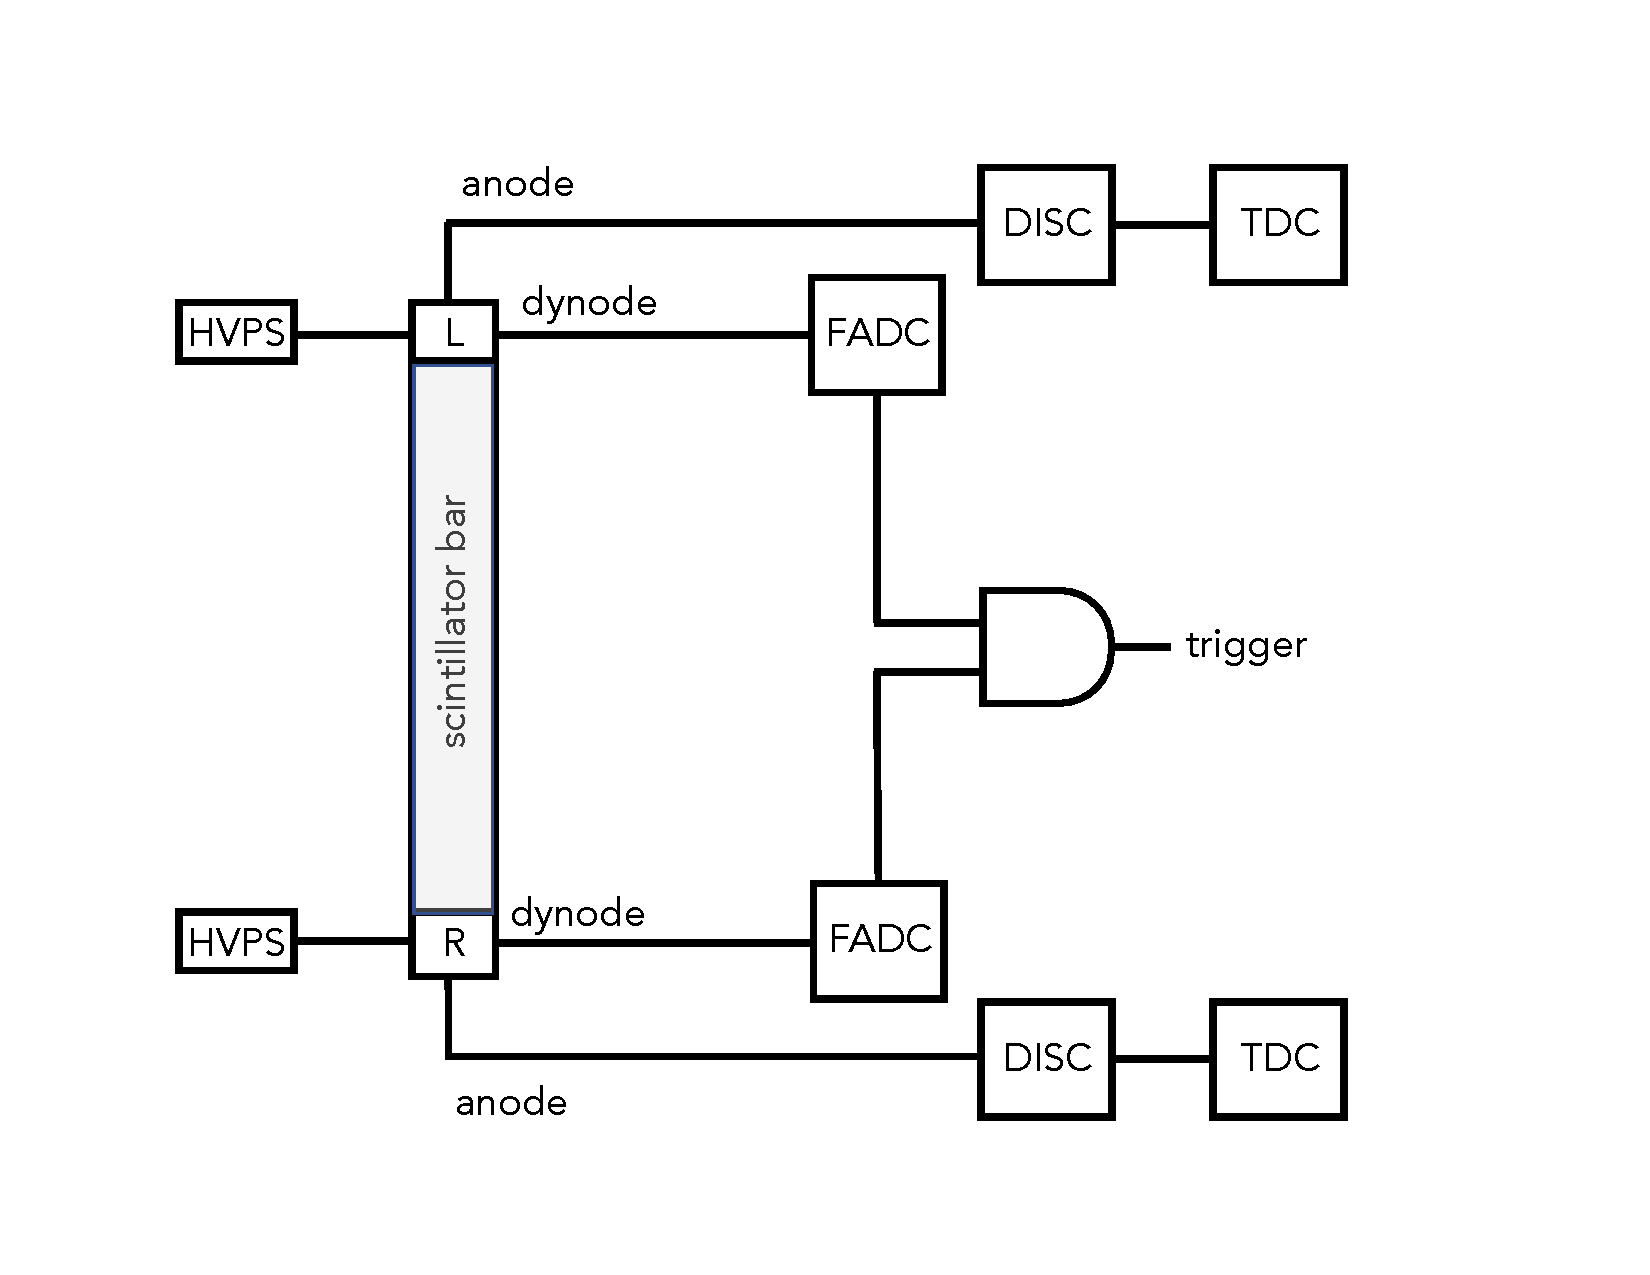
\includegraphics[width=0.39\textwidth,natwidth=610,natheight=642]{pics/ftof-electronics-block.pdf}}}
\end{picture} 
\caption{Schematic of the electronics for each counter in the CLAS12 FTOF system.}
\label{elec-block}
\end{figure}
%%%%%%%%%%%%%%%%%%%%%%%%%%%%%%%%%%%%%%%%%%%%%%%%%%%%%%%%%

The intrinsic resolution of the electronics system ($\sigma_0$) must be optimized to ensure that it does
not become a limitation to the effective counter timing resolution. There are several contributions to this
term and each electronic component was studied to understand its effect.  From our measurements on the
bench and from CLAS12, a reasonable approximation for the floor term in the counter hit time resolution
is $\sigma_0=40$~ps (see Section~\ref{res-sec}). The PMT anode outputs are connected to JLab-designed
VME leading-edge discriminators. A leading-edge rather than a constant-fraction discriminator was chosen
for the FTOF system. Although a constant-fraction discriminator delivers better timing initially, off-line
time-walk corrections to leading-edge times give comparable results at a significantly lower cost since the
off-line analysis can use the measured charge. Time walk is an instrumental shift in the measured hit time
that arises due to the finite rise time of the analog pulse. For a given event time, pulses of different
amplitude cross the leading-edge discriminator threshold at slightly different time. The time-walk correction
algorithm is described in Section~\ref{sec-tw}. The discriminator threshold was set at -25~mV, significantly
above the 2~mV noise level. This threshold corresponds to roughly 1~MeV of deposited energy, consistent
with the deposited energy threshold on the FADC readout as mentioned above. The discriminator signal output
width was set to 35~ns in order to prevent multiple outputs from the same input pulse.

The output of the discriminator goes to a CAEN VME TDC. Both high resolution TDCs (25~ps LSB CAEN
VX1290A) and lower resolution TDCs (100~ps LSB CAEN V1190A) are employed, where the lower resolution
TDCs are associated with the longer counters at large polar angles for panel-1a ($N_C = 17 \to 23$), panel-1b
($N_C = 49 \to 62$), and panel-2 ($N_C = 1 \to 5$). These multi-hit pipeline TDCs were chosen in order to
allow for readout capability in the operating luminosity of $10^{35}$~cm$^{-2}$s$^{-1}$. The TDC readout window
was set to 250~ns to ensure the full dynamic range of the data was safely in time with the trigger. The key
performance specifications of these TDC units are given in Table~\ref{tdcadc-specs}. Note that the integral
non-linearity of each TDC channel in the system was measured and corrected for using a look-up table stored in
the system memory. See Ref.~\cite{daq-nim} for more details.

The PMT dynode outputs are connected to the FADCs for the pulse charge measurement. The readout
employs JLab-designed FADC250 16-channel VME 250-MHz flash ADCs~\cite{fadc-manual}. 
Figure~\ref{fadc-pulse} shows a raw ADC pulse from a representative FTOF PMT. The pedestal is determined
event-by-event and subtracted offline. Our procedure determines the pedestal over the first 15 channels. This
average is used to determine and subtract off the baseline noise in our pulse signal region, which lies between
channels 35 and 65. The measured ADC values for each counter PMT that are referred to in this paper represent
the pedestal-subtracted pulse integral in our defined signal region. A pulse fitting algorithm, which fits the leading
edge of the pulse down to the baseline, is used to determine the hit time from the FADC signal. The readout window
for the FTOF FADCs is set to 48 samples (192~ns). The applied readout threshold is set to 1~MeV to ensure that
the hit cluster energy can be determined with a reasonable accuracy. Details on the hit clustering for FTOF are
described in Ref.~\cite{recon-nim}. The key performance specifications of these FADC units are given in
Table~\ref{tdcadc-specs}.

The signal cables used for the FTOF system to connect from the PMT anodes and dynodes to the Forward
Carriage patch panels are RG-58C/U fire-retardant coaxial cables. This type of cable is appropriate for
moderate length cable runs for fast signals with low signal-distortion requirements. The cable runs vary
from 47~ft to 59~ft. The connections from the patch panels to the readout electronics are made with a
final 5~ft run of low loss RG-174 coaxial cable. The inline signal inverting transformers for the panel-1b
dynodes (see Section~\ref{sec-elec}) were attached directly to the Forward Carriage patch panels.

%%%%%%%%%%%%%%%%%%%%%%%%%%%%%%%%%%%%%%%%%%%%%%%%%%%%%%%%
\begin{table*}[htbp]
\begin{center}
\begin{tabular}{c|c} \hline
TDC Specs (V1190A/VX1290A) & ADC Specs \\ \hline
No. Channels: 128/32             & 16               \\ 
RMS resolution 100~ps/25~ps          & Sampling 250 MHz \\
Resolution: 19~bit/21~bit                  & Resolution: 12-bit \\ 
Inter-channel isolation $\le$ 3 LSB & Clock jitter 350~fs \\ 
Double-hit resolution 5~ns          & Data memory 8~$\mu$s \\  
Full-scale range 52~$\mu$s          & Trigger/Data latency 8~$\mu$s / 32~ns \\
\multicolumn{2}{c}{Integral/Differential non-linearity} \\
$<$ 2.5 LSB / $<$ 3 LSB             & $\pm$0.5 LSB / $\pm$0.8 LSB \\
Inter-channel isolation $<$ 3 LSB   & SNR 56.8~dB @ 100~MHz input \\ \hline
\end{tabular}
\end{center}
\caption{Key performance specifications of the FTOF CAEN V1190A and VX1290A pipeline
TDCs and the JLab FADC250 flash ADCs.}
\label{tdcadc-specs}
\end{table*}
%%%%%%%%%%%%%%%%%%%%%%%%%%%%%%%%%%%%%%%%%%%%%%%%%%%%%%%%%

%%%%%%%%%%%%%%%%%%%%%%%%%%%%%%%%%%%%%%%%%%%%%%%%%%%%%%%%%
\begin{figure}[htbp]
\vspace{3.2cm}
\begin{picture}(50,50) 
\put(-45,-43)
{\hbox{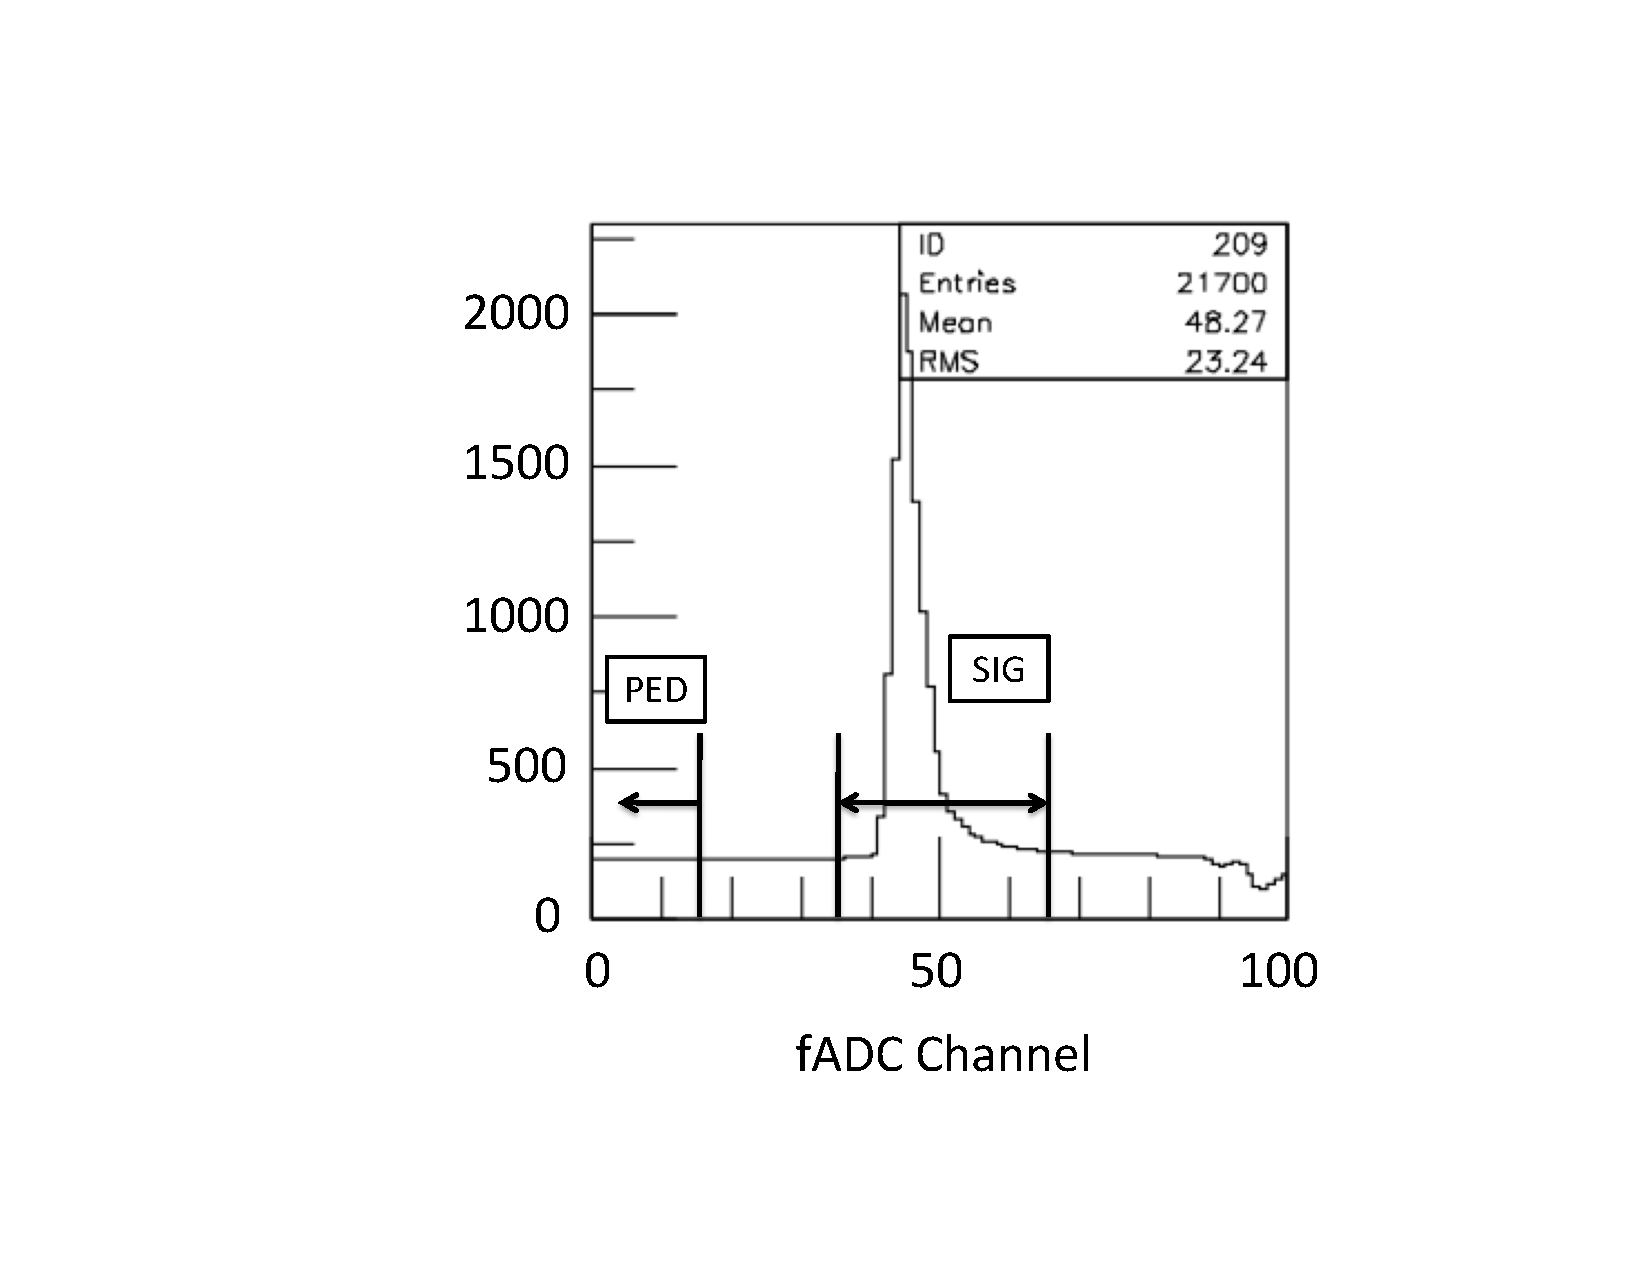
\includegraphics[width=0.46\textwidth,natwidth=610,natheight=642]{pics/fadc-pulse.pdf}}}
\end{picture} 
\caption{Typical FADC pulse for a representative FTOF counter from the JLab FADC250. The ``PED''
region is used to determine the average pedestal in the ``SIG'' region shown about the PMT pulse. This
plot shows ADC counts vs. FADC sample number (1~sample = 4~ns).}
\label{fadc-pulse}
\end{figure}
%%%%%%%%%%%%%%%%%%%%%%%%%%%%%%%%%%%%%%%%%%%%%%%%%%%%%%%%%

\subsubsection{High-Voltage Supplies}

The PMTs for the FTOF counters typically operate in the range from 1500~V to 2000~V with negative
polarity. The typical dark current drawn by the PMTs is measured to be $<$20~nA. The system is powered
by a single high voltage mainframe for each sector. These mainframes are either CAEN 1527LC or CAEN 4527
units outfitted with negative polarity 24-channel A1535N modules that can supply up to 3.5~kV per channel with
a maximum current of 3~mA. The power supply has a voltage ripple specification of $<$20~mV peak-to-peak.
Each channel consumes less than 1~W during counter operation with typical supply currents per channel between
300~$\mu$A to 500~$\mu$A.

The mainframe is controlled remotely through the Hall~B Slow Controls system. A graphical user interface
using EPICS~\cite{epics} running on a UNIX system communicates with the mainframe via Ethernet. The
mainframe settings enable basic protection of the PMTs in terms of maximum voltage and current settings,
and channel ramp rates.

The high voltage cables for each PMT are fire-retardant RG-59 coaxial cables that run from the PMT
voltage divider to a local disconnect HV distribution box located behind the panel-2 arrays in each
sector. There are four 48-channel HV distribution boxes for each sector, two for the left PMTs and two
for the right PMTs. The output of each HV distribution box is a pair of 35-ft long multi-conductor cables,
each containing 24-channels, with a Radiall connector to mate with the HV A1535N board input connector.
Each multi-conductor high voltage cable contains individual conductors wrapped in Tefzel insulation, an outer
wire shield, and a PVC insulation wrap. Each conductor is rated at 5~kV.

\section{FTOF Performance}
\label{sec:performance}

This section highlights the performance of the FTOF system both on the test bench and in Hall~B during
the first beam runs for CLAS12. The bench test timing performance is important to ensure that the
refurbished counters that make up the panel-1a and panel-2 arrays from the CLAS TOF system still meet
their original performance specifications as detailed in Table~\ref{spec-table} and Ref.~\cite{tof-nim}. These
bench performance studies are even more important for the newly constructed panel-1b arrays for CLAS12
as they are primarily responsible for the limits of the particle identification separation for CLAS12 in the
forward direction. Full details on the bench test performance results for the panel-1a and panel-2 counters
are provided in Ref.~\cite{dsc-cn2013-001} and for the panel-1b counters in Ref.~\cite{nim-p1b}.

In this section the essential performance results from the bench testing studies are presented in terms
of the counter photoelectron statistics and benchmark time calibrations. Then the calibration algorithms
are introduced to provide details on how the in-beam FTOF time resolution performance was quantified.
Finally, this section provides the current status of the particle identification capabilities of the FTOF
system in relation to the design specifications.

\subsection{Bench Measurements}

\subsubsection{Counter Photoelectron Statistics}
\label{sec:npe}

The primary approach to determine the average number of photoelectrons at the photocathode of a PMT
generated by minimum-ionizing particles passing through the scintillation bars employs the ratio of the
integral of the signal pulse to the integral of the pulse for a single photoelectron~\cite{Gi86}. For these
measurements we used a 350~MHz (4~GSa/s) oscilloscope with a pulse averaging mode and averaged over
1000 pulses. The minimum-ionizing particle signals were analyzed by connecting the scope to a PMT mounted
on one of the shortest FTOF panel-1a counters. For the single photoelectron signal, we took data using just a
bare PMT on the bench using the same HV setting. For both measurements the oscilloscope threshold was
adjusted appropriately. For the minimum-ionizing peak analysis the threshold had to be set high enough
($>$200~mV) to eliminate tracks that did not pass through the full thickness of the bar. For the single
photoelectron peak the threshold had to be set low enough (1~mV) to pick out the single-electron emission
noise pulses from the photocathode that are the dominant source of the PMT intrinsic dark current. This
somewhat crude measurement scheme yielded $N_{pe}$=1000$\pm$100, a value consistent with that found
during the initial characterization of the number of photoelectrons seen by the PMTs for these counters for
the CLAS TOF system~\cite{tof-nim}. Based on the parameterization given in Eq.(\ref{nphe-eq}),
Fig.~\ref{nphe-plot} shows the number of photoelectrons at the PMT photocathodes for the different FTOF
counters.

%%%%%%%%%%%%%%%%%%%%%%%%%%%%%%%%%%%%%%%%%%%%%%%%%%%%%%%%%
\begin{figure}[htbp]
\vspace{2.2cm}
\begin{picture}(50,50) 
\put(5,-45)
{\hbox{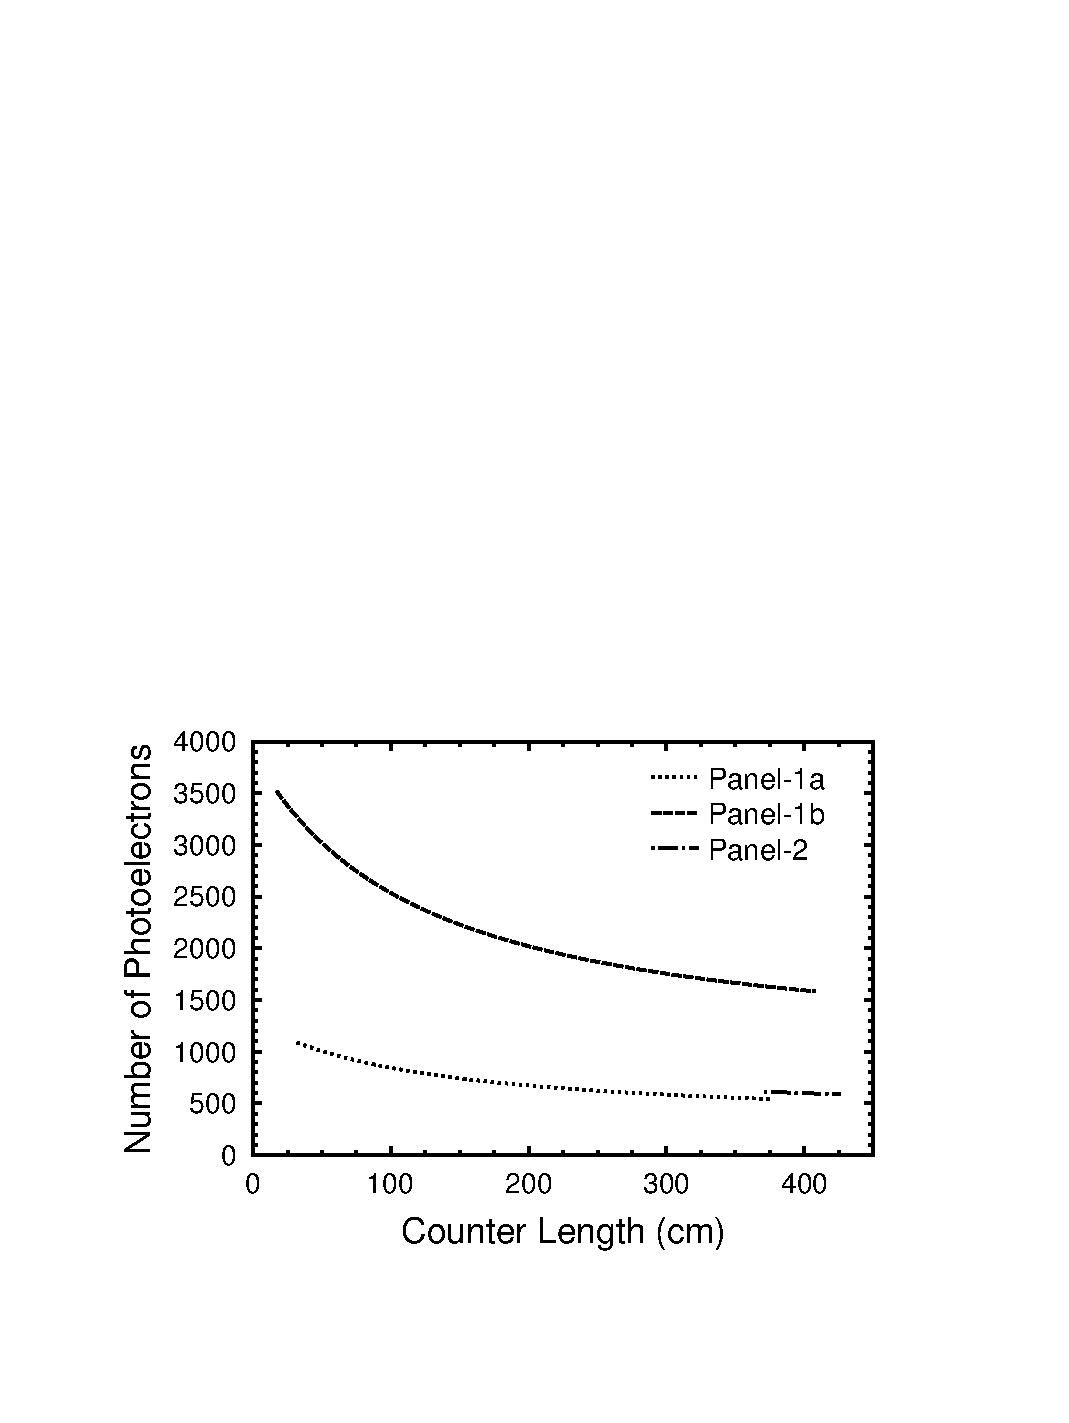
\includegraphics[width=0.6\textwidth,natwidth=610,natheight=642]{pics/nphe.pdf}}}
\end{picture} 
\caption{Parameterized distribution of the number of photoelectrons vs. counter length (cm) for the
panel-1a (dotted), panel-1b (dashed), and panel-2 (dot-dashed) counters based on direct measurements
with the shortest panel-1a counter.}
\label{nphe-plot}
\end{figure}
%%%%%%%%%%%%%%%%%%%%%%%%%%%%%%%%%%%%%%%%%%%%%%%%%%%%%%%%%

A second method to estimate the number of photoelectrons produced at the PMT photocathode,
which accounts for the quantum efficiency at the photocathode, can be estimated from cosmic
ray data using the form of Ref.~\cite{kajino}:

\begin{equation}
\label{nphe}
\langle N_{pe} \rangle = \left( \frac{M_{ADC}}{\sigma_{ADC}} \right)^2,
\end{equation}

\noindent
where $M_{ADC}$ is the ADC mean for the minimum-ionizing peak in the ADC spectrum and $\sigma_{ADC}$
is the width of the ADC distribution. The form of Eq.(\ref{nphe}) assumes that a finite $\sigma_{ADC}$
arises solely due to statistical variations in the number of photoelectrons created at the photocathode for
an event sample with a fixed energy loss per track, which we can assume to be a good approximation for
perpendicularly incident minimum-ionizing tracks. From the measured data averaged across the counters in
panel-1a and panel-1b it was found that $N_{pe}^{1a} = 373 \pm 39$ and $N_{pe}^{1b} = 1158 \pm 77$
\cite{pmt-currents}. These results, while roughly a factor of two below the parameterized estimates, also
show the same factor of three difference in the expected number of photoelectrons for panel-1b relative
to panel-1a. The estimates from the first approach are considered to be more reliable not only because they
are connected to a more direct measurement of the number of photoelectrons, but also because this
parameterization for $N_{pe}$ used in Eq.(\ref{timing-func}) agrees reasonably well with the measured
counter resolutions shown in Section~\ref{tres-beam}.

\subsubsection{Bench Time Resolution Performance}
\label{sec-bench}

The basic algorithm used on the test bench for the panel-1a and panel-2 counters to determine the time
resolution of a given reference counter was to use cosmic ray tracks to compare the measured time for a
reference counter to the time measured by two other identical counters in a triplet counter configuration
(see Fig.~\ref{triplet}). For a triplet measurement, where the track passes through all three counters with
double-sided readout, six times are measured ($t_1 \to t_6$). Each time measurement actually represents
the difference between the discriminated PMT signal (TDC start) and the trigger time (TDC stop)
generated from the six-fold PMT coincidence. These time measurements are then translated into three
counter hit times $t_{t,m,b} = \frac{1}{2}(t_{1,3,5} + t_{2,4,6})$.

%%%%%%%%%%%%%%%%%%%%%%%%%%%%%%%%%%%%%%%%%%%%%%%%%%%%%%%%%
\begin{figure}[htbp]
\vspace{2.0cm}
\begin{picture}(50,50) 
\put(30,0)
{\hbox{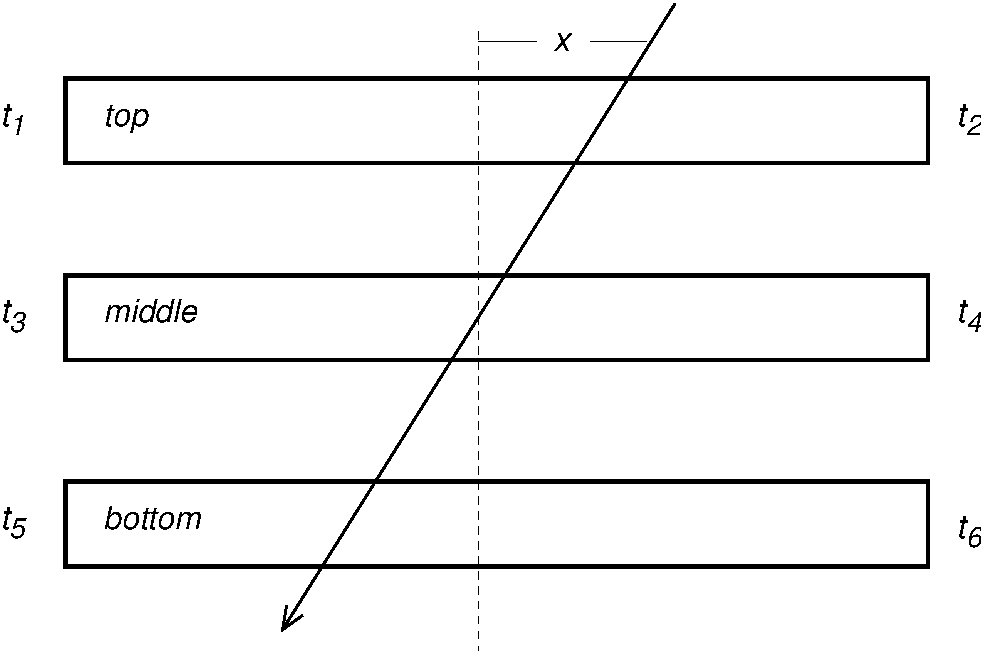
\includegraphics[width=0.45\textwidth,natwidth=610,natheight=642]{pics/triplet-alt.pdf}}}
\end{picture} 
\caption{Schematic representation of a triplet of counters (labeled top - $t$, middle - $m$, and bottom
- $b$) with a cosmic ray track traversing the stack. The geometry of the triplet was configured such that
the counters were equally spaced.}
\label{triplet}
\end{figure}
%%%%%%%%%%%%%%%%%%%%%%%%%%%%%%%%%%%%%%%%%%%%%%%%%%%%%%%%%

For incident tracks that pass fully through each counter of the triplet, we can define a time residual

\begin{equation}
\label{res-time}
t_r = t_m - \frac{1}{2}(t_t + t_b),
\end{equation}

\noindent
where the time $t_m$ of the middle scintillator hit should be the average of the measured times $t_t$ and
$t_b$ for the top and bottom scintillator hits, respectively. Thus the measured residual $t_r$ should nominally
be zero. However, due to the smearing of the measured times $t_t$, $t_m$, and $t_b$ due to the finite time
resolution of the measurements, the residual time $t_r$ will also be smeared. The width of the $t_r$
distribution can be used to determine the average time resolution of the counters in the triplet.

The average time resolution of each of the identical counters was computed from the variance $\delta t_r$
of the measured time residual $t_r$ summed over all the full event sample (see Fig.~\ref{resid} for a
representative result). Assuming the average time resolution for each PMT in the triplet is identical and
taking into account that each counter is read out using two PMTs, we can write the final expression for the
average counter time resolution as:

\begin{equation}
\label{sig-counter}
\sigma_{counter} = \frac{2}{\sqrt{6}} \delta t_r.
\end{equation}

\noindent
Thus a measure of the variance of the time residual distribution provides a measure of the average
resolution of a counter in the triplet. 

%%%%%%%%%%%%%%%%%%%%%%%%%%%%%%%%%%%%%%%%%%%%%%%%%%%%%%%%%
\begin{figure}[htbp]
\vspace{1.9cm}
\begin{picture}(50,50) 
\put(-28,-135)
{\hbox{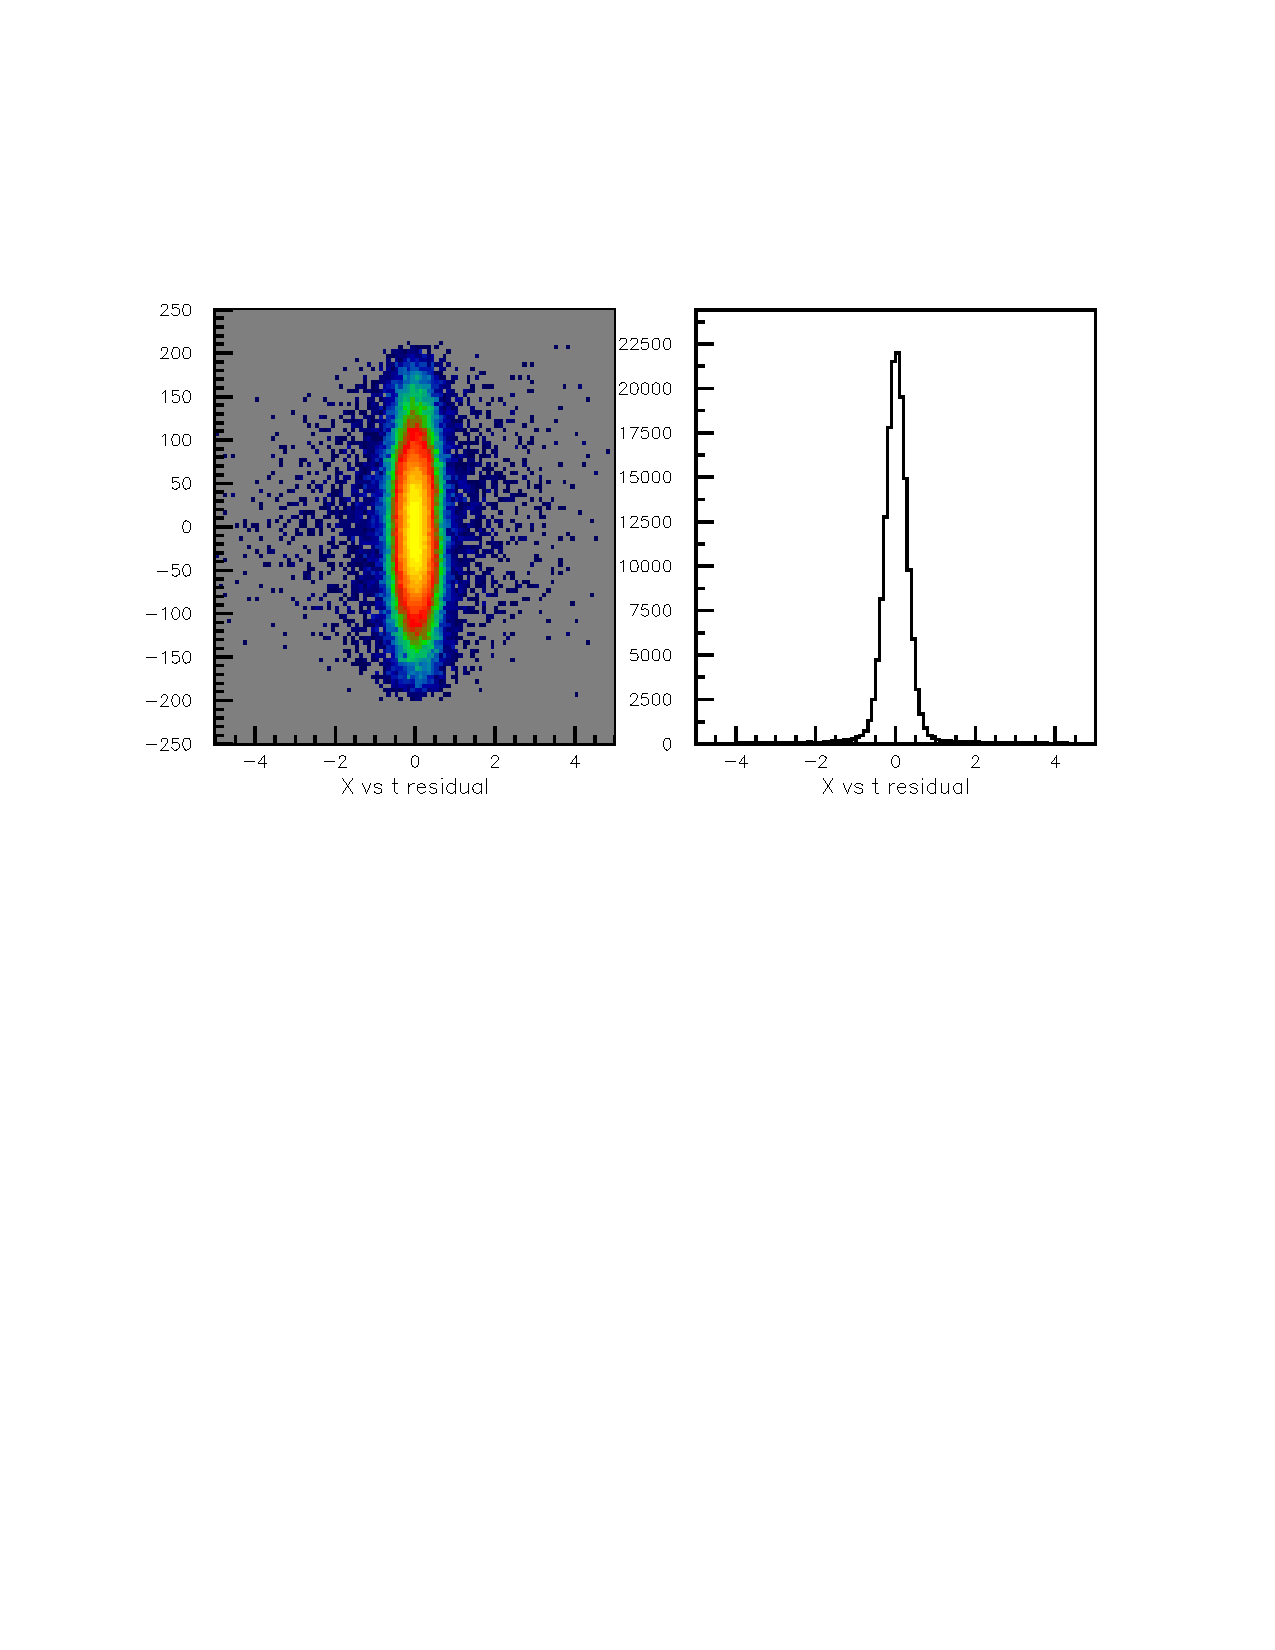
\includegraphics[width=0.6\textwidth,natwidth=610,natheight=642]{pics/residual-2d.pdf}}}
\end{picture} 
\caption{Data from the S2-S4-S3 panel-1a triplet for counter \#23. (Left) Plot of the triplet hit
coordinate (cm) (defined from the hit in the middle counter of the triplet) vs. the time residual
$t_r$ (ns). (Right) The triplet time residual $t_r$ distribution (ns) that is fit to determine the
average counter timing resolution using Eq.(\ref{sig-counter}).}
\label{resid}
\end{figure}
%%%%%%%%%%%%%%%%%%%%%%%%%%%%%%%%%%%%%%%%%%%%%%%%%%%%%%%%%

Figure~\ref{final-resolution} shows the average time resolution measured in the triplet configurations
for the panel-1a and panel-2 FTOF counters. For these measurements the fully assembled counter arrays
were stacked one above the other in the cosmic ray test stand. The triplets $t$, $m$, and $b$ were
formed from the counters for sectors~1, 6, and 5 and separately for the counters for sectors~2, 4, and
3. This analysis included a minimum PMT ADC cut to remove events that did not pass through the full
thickness of the counter (``corner-clippers'') and also included a coordinate cut of $\pm$10~cm about
the center of the scintillation bar. Due to the use of leading edge discriminators, the measured PMT times
were corrected with a power-law time-walk function of the form:

\begin{equation}
\label{walk-function}
t_{walk}^{L,R} = \frac{A_0}{1 + A_1 \sqrt{(ADC - PED)_{L,R}}}.
\end{equation}

\noindent
Here, $ADC - PED$ is the pedestal-subtracted ADC value for each PMT (i.e. the pedestal-subtracted
integral of the SIG region in Fig.~\ref{fadc-pulse}). The parameters $A_0$ and $A_1$ were determined
by fitting the residual times for the left and right PMTs of a given counter from Eq.(\ref{res-time}) vs.
$ADC_L$ and $ADC_R$ after the PMTs of all counters were gain-matched. See Ref.~\cite{dsc-cn2013-001}
for full details on these measurements.

The average time resolutions for the counters in the panel-1a and panel-2 triplets were found to be within
20\% of those achieved for the original CLAS TOF baseline measurements~\cite{tof-nim}. However, when
accounting for the different TDC LSB contribution to the floor term (25~ps/100~ps for CLAS12 and
50~ps for CLAS) the results agree remarkably well.

%%%%%%%%%%%%%%%%%%%%%%%%%%%%%%%%%%%%%%%%%%%%%%%%%%%%%%%%%
\begin{figure}[htbp]
\vspace{5.3cm}
\begin{picture}(50,50) 
\put(25,52)
{\hbox{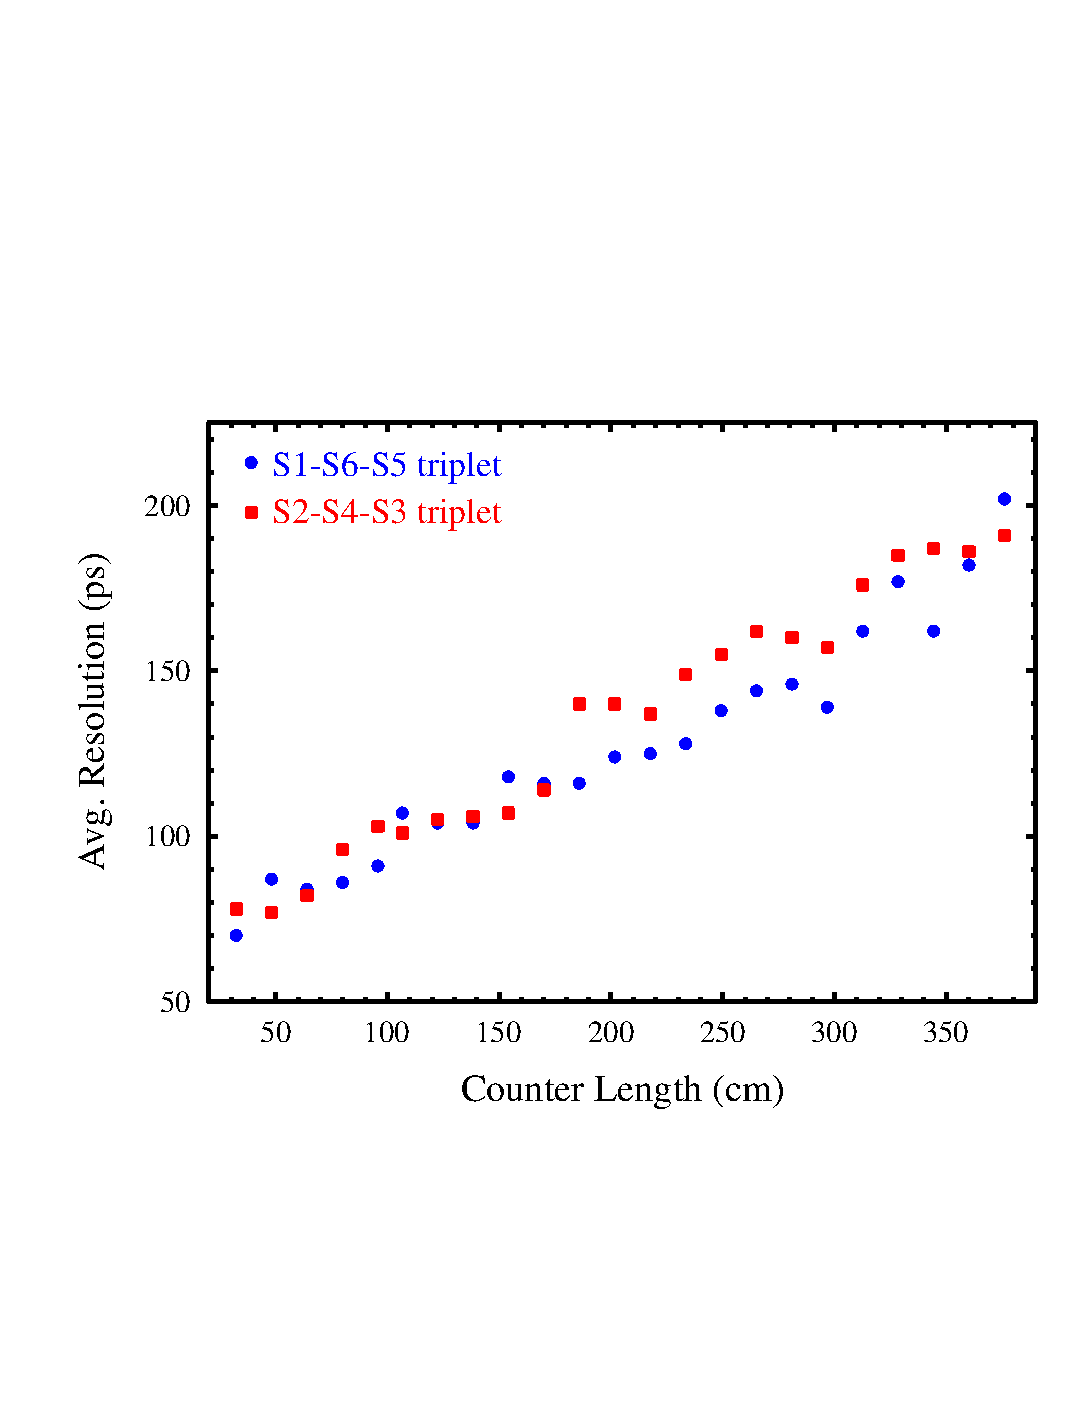
\includegraphics[width=0.40\textwidth,natwidth=610,natheight=642]{pics/p1a-tres.pdf}}}
\put(25,-55)
{\hbox{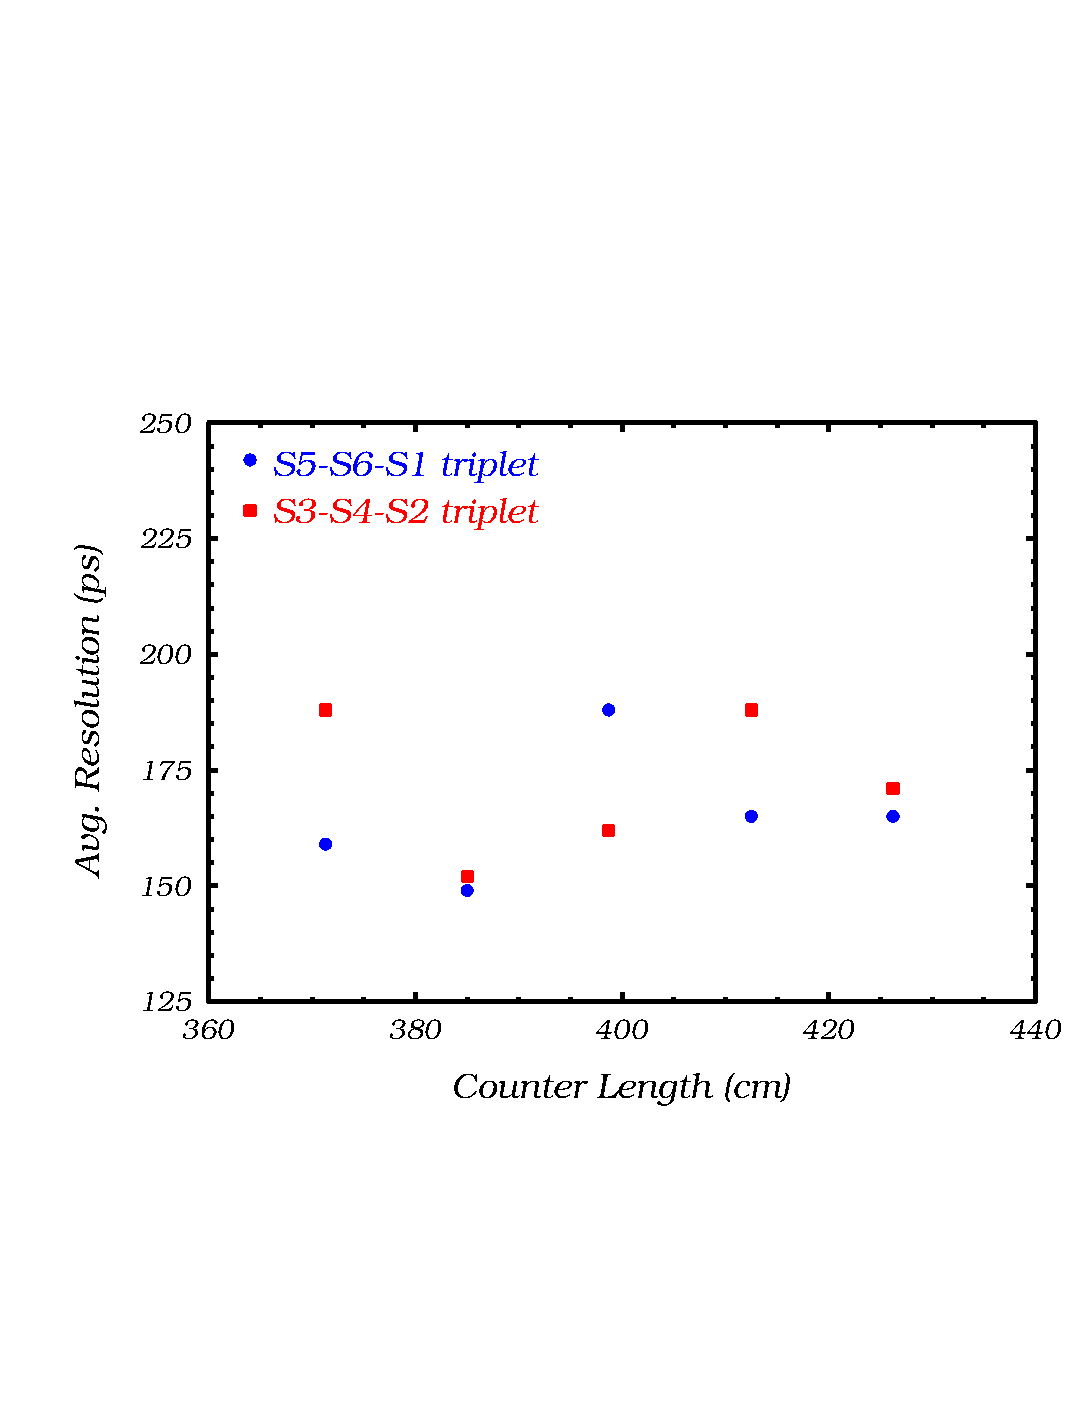
\includegraphics[width=0.40\textwidth,natwidth=610,natheight=642]{pics/p2-tres.pdf}}}
\end{picture} 
\caption{Average bench measurement resolutions (ps) vs. counter length (cm) using cosmic rays for the
refurbished FTOF panel-1a (top) and panel-2 (bottom) counters. The different sets of data points
correspond to the two different cosmic ray test stands used for calibration. The data points for the
counters in sectors 1, 5, and 6 were averaged together, as well as those for the counters in sectors 2, 3,
and 4.}
\label{final-resolution}
\end{figure}
%%%%%%%%%%%%%%%%%%%%%%%%%%%%%%%%%%%%%%%%%%%%%%%%%%%%%%%%%

The bench measurements for the panel-1b FTOF counters were carried out using a stack of six
equidistant counters of a given counter number from $N_C = 1 \to 62$. Accounting for the
necessary path length corrections to relate the individual counter times to each other, six simultaneous
triplet counter measurements were analyzed and the resulting time-residual system of equations was then
solved for the individual counter time resolution. Also in distinction to the simple time-walk correction
employed for the panel-1a and panel-2 measurements shown in Eq.(\ref{walk-function}), a more sophisticated
position-dependent time-walk correction was employed that generalizes the simpler position-independent form.
Precision measurements of the time-walk amplitude ($A_0$ in Eq.(\ref{walk-function})) vs. the distance from
the PMT showed a nearly linear fall-off of the amplitude with increasing distance from the PMT. On average
the time-walk amplitude is $\sim$30\% larger at the PMT compared to the far end of the bar, although this
near to far end ratio of the amplitude decreases linearly with the length of the bar. Our measurements
showed this ratio varies between 20\% for the shortest bars to 40\% for the longest bars. After accounting
for this correction vs. hit position along the bar, a final baseline for the average panel-1b time resolutions was
extracted averaging over the six counters of a given number from $N_C = 1 \to 62$. The resulting time
resolutions for the panel-1b counters are shown in Fig.~\ref{p1b-tres} and range from 30~ps for the shortest
counters  (17~cm long) to 80~ps for the longest counters (408~cm long). Full details describing the
measurements are provided in Ref.~\cite{nim-p1b}.

%%%%%%%%%%%%%%%%%%%%%%%%%%%%%%%%%%%%%%%%%%%%%%%%%%%%%%%%%%%
\begin{figure}[htbp]
\vspace{2.3cm}
\begin{picture}(50,50) 
\put(10,-67)
{\hbox{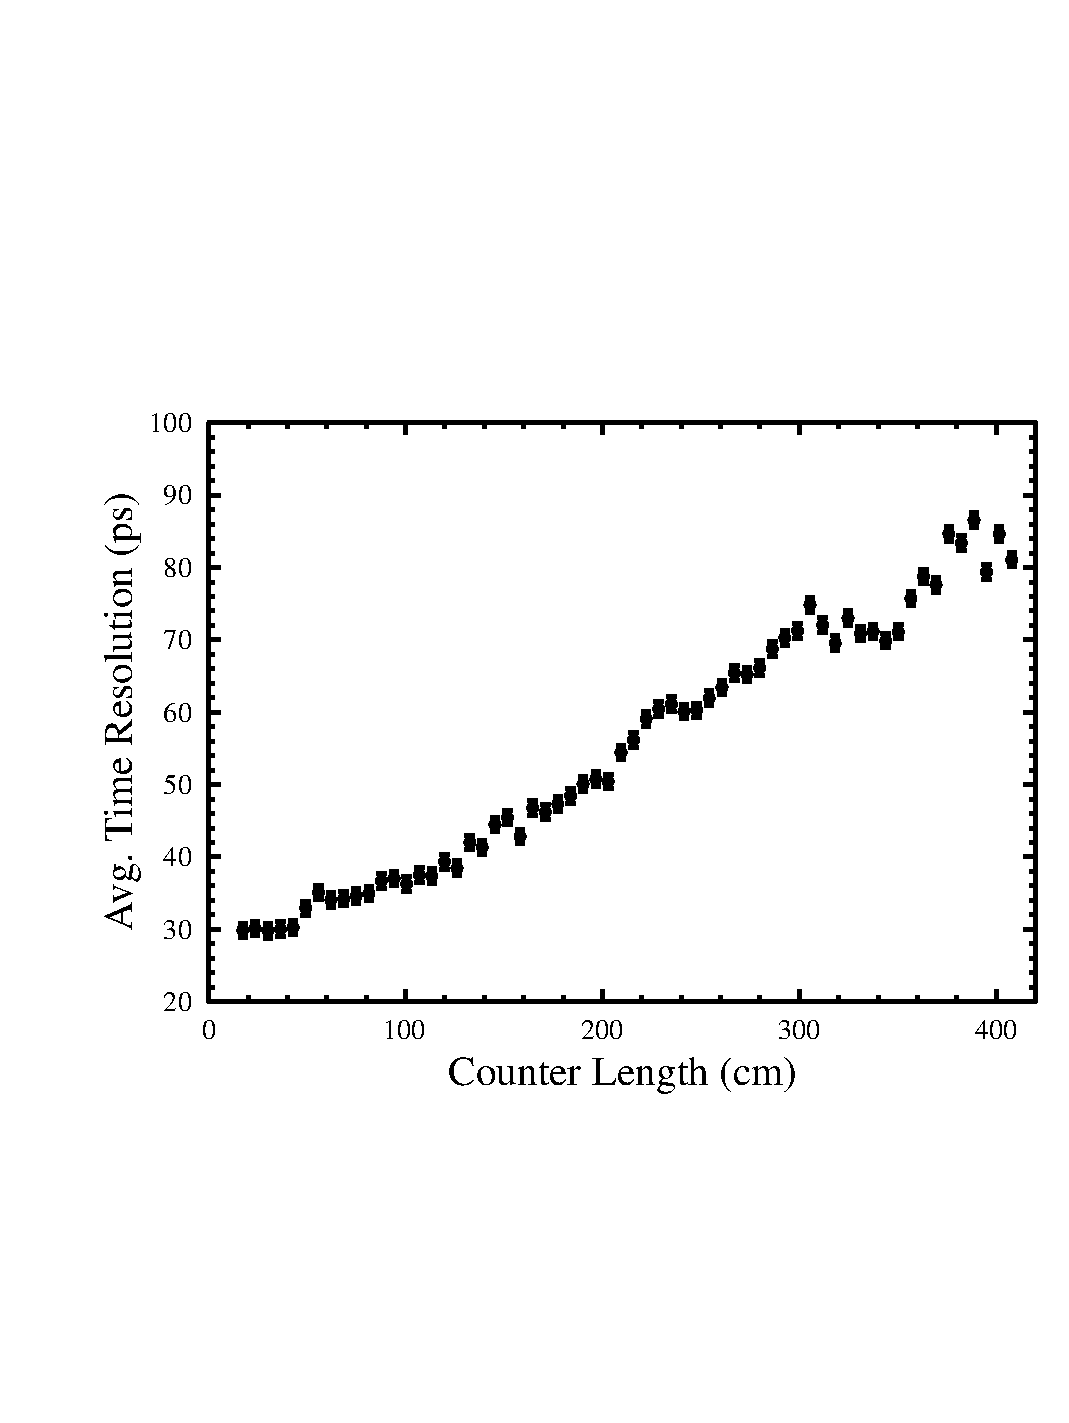
\includegraphics[width=0.5\textwidth,natwidth=610,natheight=642]{pics/p1b-tres.pdf}}}
\end{picture} 
\caption{Measurements of the time resolution (ps) vs. counter length (cm) achieved for the FTOF panel-1b
system averaged over the six counters of a given length belonging to each CLAS12 Forward Carriage sector.
These data were acquired on the bench using cosmic rays. Full details are included in Ref.~\cite{nim-p1b}.}
\label{p1b-tres}
\end{figure}
%%%%%%%%%%%%%%%%%%%%%%%%%%%%%%%%%%%%%%%%%%%%%%%%%%%%%%%%%%%

For our purposes in quoting counter time resolution values, it is essential to distinguish between two
different quantities. The first is the {\em intrinsic} counter time resolution that reflects the resolution
parameterized in Eq.(\ref{timing-func}). This includes the resolution contributions that mainly depend on
the photon statistics at the PMT photocathode and hence the counter geometry, surface quality, scintillation
material and bulk quality, wrapping preparations, etc., the transit time spread of the PMT, and the readout
electronics noise (the floor term of the resolution). However, when calibrating the counter timing in situ in
Hall~B with beam interactions in the experimental target, an {\em effective} time resolution is extracted that
includes not only the intrinsic resolution contributions, but also contributions from the angle-dependent
uncertainty in the path length determined by the CLAS12 forward tracking system and the resolution spread
in the accelerator RF signal that is used as a comparison reference time. The results quoted in this section
represent the intrinsic time resolutions of the counters. The effective in situ time resolutions are discussed
in Section~\ref{tres-beam}.

\subsection{FTOF Beam-Data Calibrations}
\label{beam-data-calib}

In the nominal data taking mode for CLAS12, whenever the FTOF is involved in an event that triggers the
spectrometer readout, the ADCs and TDCs for all PMTs with a signal above the readout threshold are
recorded. For the FADCs, the charge of the pulse is integrated over the extent of the pulse region and the
pedestal is subtracted event by event during offline data processing as discussed in Section~\ref{sec-elec}.
For the TDCs the time recorded is relative to the trigger. To determine the flight time of the charged track
from the target to the FTOF, the TDC time must be correlated with the time of the electron beam bunch
initiating the trigger that is defined by the accelerator radio frequency (RF) pulse. The RF signal from the
accelerator has a period of 2.004~ns. The RF bunch length itself corresponds to about 2~ps. Although
the signal timing is very accurate (with a resolution of $<$20~ps), the determination of which beam bunch
produced a given interaction must be determined by the experiment. Note that for the initial beam operations
with CLAS12 the electron beam was actually delivered in every other beam bunch, resulting in an effective
$T_{RF}$ of 4.008~ns.

%%%%%%%%%%%%%%%%%%%%%%%%%%%%%%%%%%%%%%%%%%%%%%%%%%%%%%%%%%%
\begin{figure}[htbp]
\vspace{2.1cm}
\begin{picture}(50,50) 
\put(-35,-68)
{\hbox{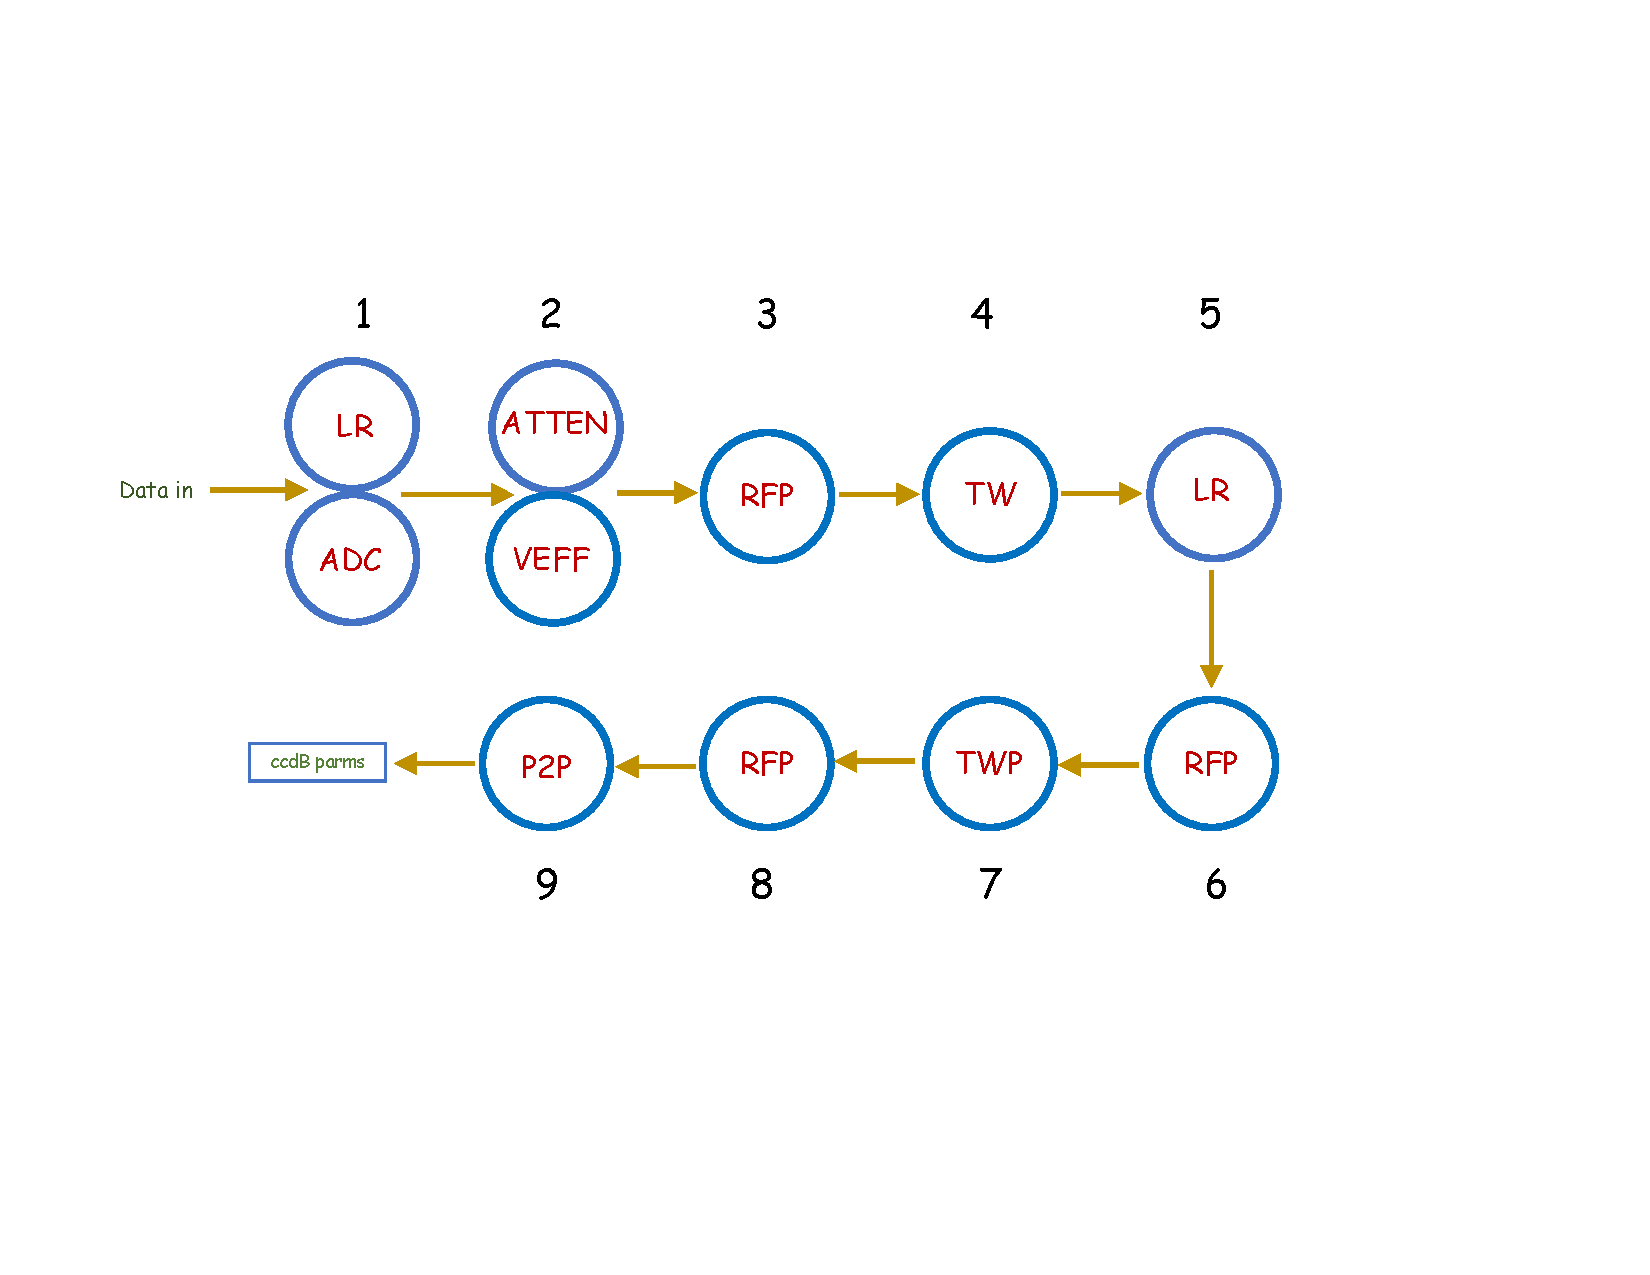
\includegraphics[width=0.5\textwidth,natwidth=610,natheight=642]{pics/calib-seq.pdf}}}
\end{picture} 
\caption{Schematic representation of the different steps in the FTOF calibration sequence and their
order. See Section~\ref{beam-data-calib} for full details.}
\label{calib-seq}
\end{figure}
%%%%%%%%%%%%%%%%%%%%%%%%%%%%%%%%%%%%%%%%%%%%%%%%%%%%%%%%%%%

The full calibration of each of the FTOF counters involves a number of discrete steps that are carried out
sequentially for a given data run (where a run typically lasts for about two hours of data collection). The
associated calibration constants for each run are stored in the CLAS12 calibration database (ccdB)
\cite{recon-nim}. After the calibration of a given data reference run is completed, the calibrations for
subsequent data runs are only carried out if there is a response shift outside of our allowed timing or
energy tolerances (which are typically 5\%). The steps to complete the FTOF calibration are carried out in
a particular sequence as detailed in Ref.~\cite{ftof-calib} and shown schematically in the calibration flowchart
of Fig.~\ref{calib-seq}. The individual steps include:

\begin{enumerate}
\item Left/right PMT time offsets (LR): This time offset accounts for the difference in the time recorded
between the left side and right side PMTs in a given counter due mainly to the different PMT transit times.
These time offsets are determined from the centroid of the difference between the left/right TDC time
difference and the left/right side hit times computed using the counter hit point from the forward tracking
system divided by the effective speed of light in the counter. These time offsets range between $\pm$5~ns.
This step is carried out initially in order to compute a hit coordinate from the FTOF information for the
effective velocity determination and then a second time to account for the fact that the time-walk correction
shifts the measured left and right PMT times.

\item ADC Calibration (ADC): Determine the ADC value to energy deposition calibration factor for each counter
using minimum-ionizing events; see Section~\ref{gain-matching}.

\item Attenuation Length Calibration (ATTEN): This property of the counter quantifies the light absorption
length in the scintillation bars and is determined by relating the measured ADC as a function of hit coordinate
along the bar; see Section~\ref{sec:attlen}.

\item Effective Velocity Calibration (VEFF): Determine the effective speed of light propagation along the counter;
see Section~\ref{sec:veff}.

\item Time-Walk Amplitude Calibration (TW, TWP): Compare the measured hit time with respect to the measured
ADC to determine the time-walk correction; see Section~\ref{sec-tw}.
  
\item Counter-to-Counter Time Offset Calibration (RFP, P2P): In order to measure the absolute flight time of a
charged particle from the target to the FTOF counter and to be able to reconstruct exclusive events when hits
are associated with multiple FTOF counters, the relative time offsets of each counter relative to all of the other
counters in the system need to be determined. This is done in two steps. The first step is to correlate each counter
hit time to the RF time, which amounts to a precision time alignment in bins of the TDC LSB. The second step is a
coarse alignment of each counter hit time in bins of the RF period $T_{RF}$; see Section~\ref{sec-talign}. During
this step the effective counter time resolutions are extracted; see Section~\ref{tres-beam}.

\item TDC Calibration (TDC): After calibrating the integral non-linearities of each TDC channel in the system
(see Section~\ref{sec-elec}), the TDC channel to time calibration is completed using beam events; see
Section~\ref{sec-tdccal} for details and a note of why this step is not included on the Fig.~\ref{calib-seq}
flowchart.

\end{enumerate}

The calibration flowchart of Fig.~\ref{calib-seq} shows that the calibrations are completed in nine separate
calibration steps that proceed in series. The data run is analyzed to complete a given step and the determined
parameters are then used in the subsequent steps. Due to dependencies of the steps on each other, several
calibration steps (LR, RFP) have to be completed multiple times. As the FTOF calibration relies on accurate
path length measurements for the forward-going charged tracks, the drift chamber calibrations are completed
before the FTOF calibrations in the overall CLAS12 subsystem calibration sequence.

To calibrate the FTOF system, events are selected that have a good electron reconstructed in the forward
direction as determined by the CLAS12 Event Builder (see Ref.~\cite{recon-nim} for details). From these events
the panel-1a and panel-1b counters are calibrated using forward-going charged leptons and pions. For the panel-2
calibration it is necessary to select charged pions and protons, as CLAS12 cannot cleanly identify leptons when
there is no electromagnetic calorimeter signal. Due to the increased energy loss and Coulomb multiple scattering
of the proton sample, the effective counter time resolutions derived for the panel-2 counters are noticeably
worse than for the bench test results using cosmic rays.

The average hit time resolution for the FTOF from the TDCs is about 80~ps and that from the FTOF
FADCs, given the rapid rise time of the fast PMT signals that provide for only 2-3 samples on the rising
edge, is only about 1~ns. A matching requirement of 10~ns between the TDC time and the FADC time is
employed during event reconstruction. While this matching requirement still needs to be tuned further,
it is already reasonably effective in allowing the FADC hits to be matched with their corresponding TDC
hits. This is important, as due to the slightly different thresholds on the discriminators and the FADCs, the
number of entries in the hit lists can be up to a factor of two different. The matching criteria is also
essential in order to assign the correct ADC information to the hit not only for the time-walk correction
that directly uses the measured ADC, but also for the energy loss computation.

\subsubsection{PMT Gain Matching}
\label{gain-matching}

One of the purposes of gain matching the FTOF PMTs is to equalize the detector response to tracks that
cross the FTOF arrays such that two counters are involved. This is a necessary procedure because each
counter must contribute equally to the trigger for a common-threshold discriminator level~\cite{trigger-nim}.
Gain matching, so that the minimum-ionizing particle peak response appears at the same ADC value for all
counters, also allows for easier data monitoring during online and offline analyses.

The FTOF PMT high voltage settings were determined using calibration runs employing minimum-ionizing
tracks. These tracks deposit roughly 10~MeV (12~MeV) as they pass through the 5-cm (6-cm) thick FTOF
scintillation bars, as $dE/\rho dx = 2$~MeV/g/cm$^2$ for minimum-ionizing particles. The high voltage
settings were initially based on runs using cosmic rays with the readout based on a calorimeter pixel trigger
(see Ref.~\cite{ec-nim}) that effectively select tracks approximately perpendicular to the face of the FTOF
counters in panel-1a and panel-1b. Currently the calibrations are carried out using minimum-ionizing tracks from
beam data coming from the target. In this case the integral of the ADC pulse is scaled by a path length
correction given by $t/p$, where $t$ is the counter thickness and $p$ is the path-length of the track in the
counter as determined by extrapolation of the drift chamber track to the location of the FTOF counter. The
energy deposited in the scintillation bars is recorded by the ADCs,  which show Landau peaks above the pedestal.
Minimum-ionizing tracks that do not pass through the full counter thickness and more heavily ionizing tracks give
rise to a background beneath the Landau peak.

In the determination of the high voltage settings, to avoid issues with the attenuation of light for tracks that
pass near the ends of the bars and with unbalanced light entering the left and right PMTs, we combine the
information from the left and right PMTs to produce an average ADC spectrum for the counter through the
quantity known as the geometric ADC mean:

\begin{equation}
\label{adc}
\overline{ADC} = \sqrt{ (ADC - PED)_L \cdot (ADC - PED)_R}.
\end{equation}

Given the finite dynamic range of the ADC, we have chosen to position the minimum-ionizing peak in a
particular ADC value that is different for the panel-1a, panel-1b, and panel-2 counters. For all counters
this value is selected so that it is safely above the pedestal, but leaves sufficient range for the more
highly ionizing charged tracks of our typical physics events. To minimize PMT aging effects that result in
loss of PMT gain with time correlated with the total charge collected at the anode of the PMT, the gains
are set as low as possible.

The position of the minimum-ionizing peak in the $\overline{ADC}$ spectrum is set by the PMT HV values.
For a given scintillation bar, a typical $\overline{ADC}$ spectrum is shown in Fig.~\ref{gmean}. Given that
the same ADC geometric mean value is chosen to position the minimum-ionizing peak for all counters in either
panel-1a or panel-1b, the required PMT gain increases linearly from the short to the long bars to compensate
for the attenuation losses in the longer bars.

%%%%%%%%%%%%%%%%%%%%%%%%%%%%%%%%%%%%%%%%%%%%%%%%%%%%%%%%%
\begin{figure}[htbp]
\vspace{2.6cm}
\begin{picture}(50,50) 
\put(35,-46)
{\hbox{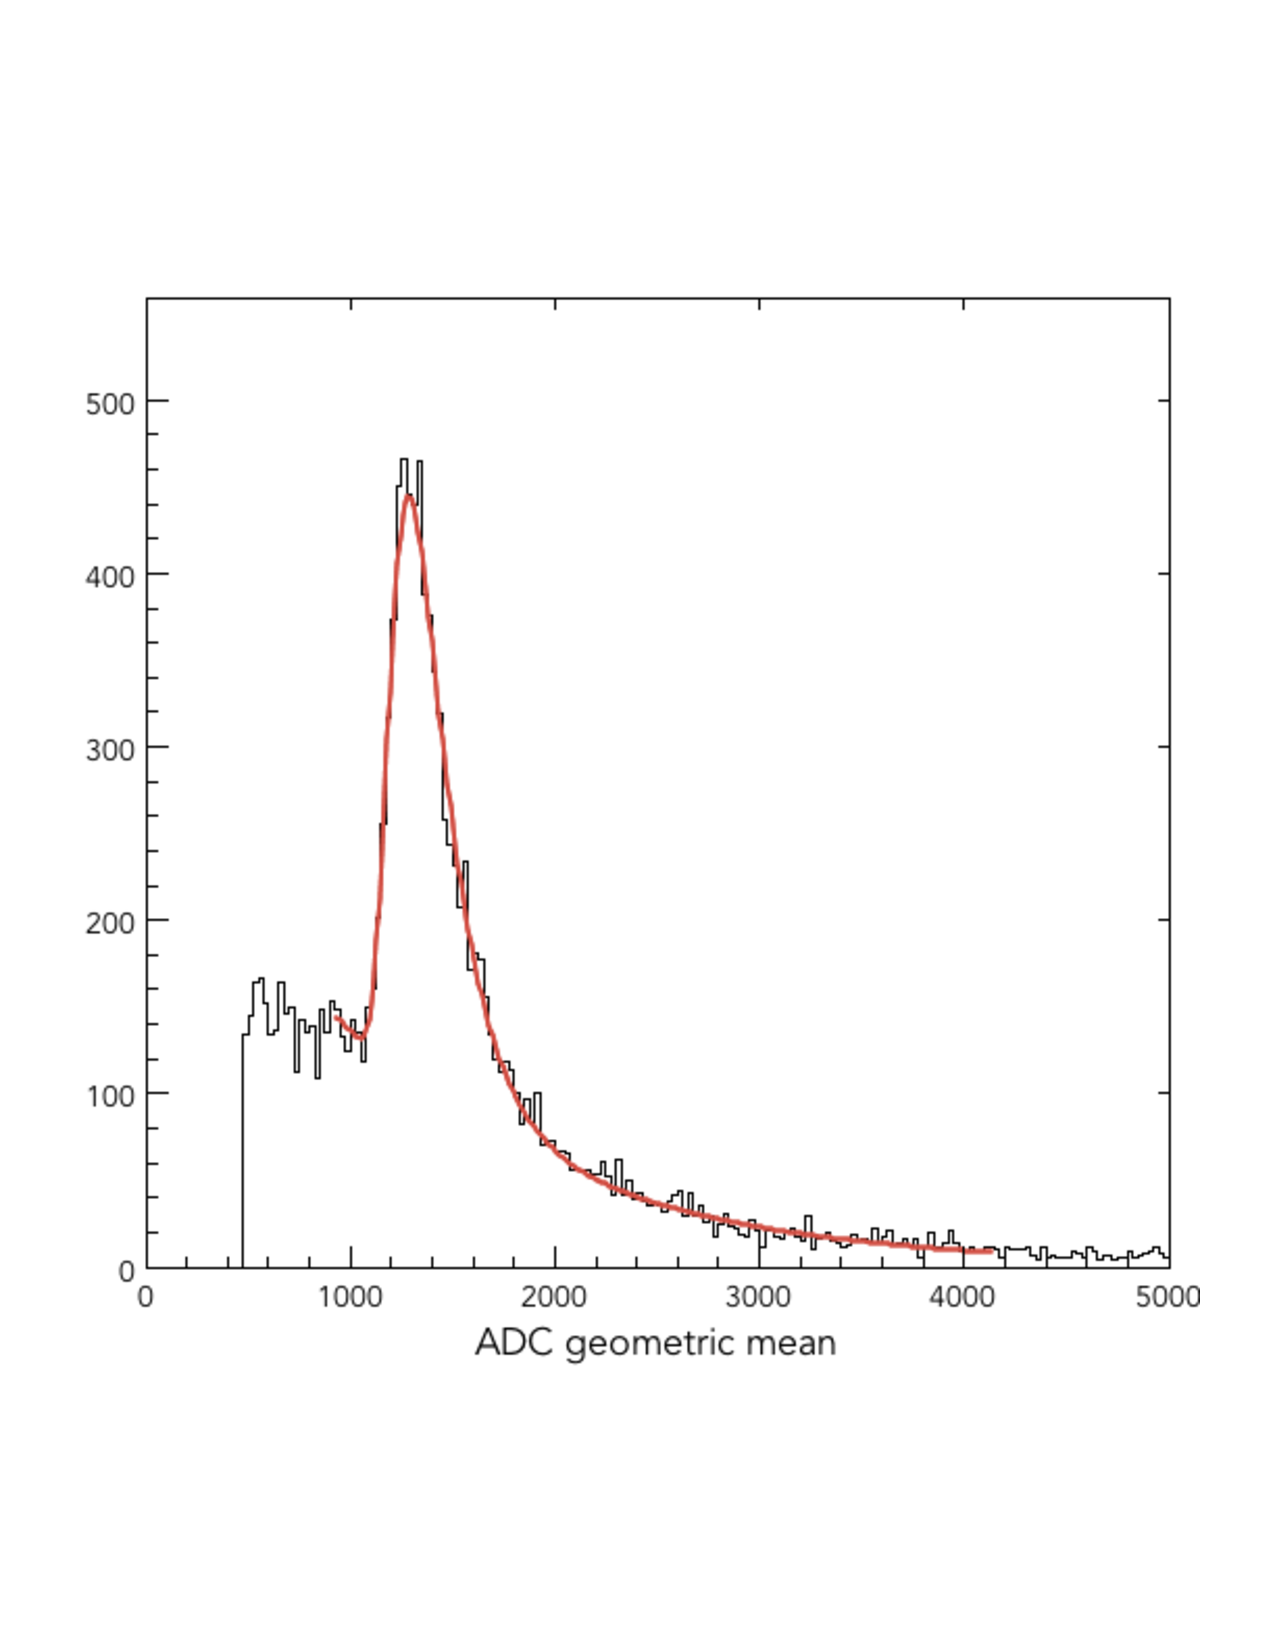
\includegraphics[width=0.34\textwidth,natwidth=610,natheight=642]{pics/gmean.pdf}}}
\end{picture} 
\caption{Geometric ADC mean spectrum for one representative FTOF counter from beam data. The
recorded events are pedestal subtracted. The red curve is a fit function that includes a Landau shape
for the peak and an exponential for the background.}
\label{gmean}
\end{figure}
%%%%%%%%%%%%%%%%%%%%%%%%%%%%%%%%%%%%%%%%%%%%%%%%%%%%%%%%%

The gain $G$ of a PMT can be related to the high voltage setting $V$ using $G \propto V^\alpha$, which
represents a basic power law form with $\alpha$ the power law factor.  This expression governs the gain
change for a given change in voltage. With this expression, the PMT gain $G_1$ at a given voltage $V_1$ can
be related to the gain $G_2$ at a different voltage $V_2$ using:

\begin{equation}
\label{power-law}
\frac{G_1}{G_2} = \left( \frac{V_1}{V_2} \right) ^\alpha,
\end{equation}

\noindent
which can be rewritten in a slightly different form as:

\begin{equation}
\label{delta}
\frac{\Delta G}{G} = \alpha \frac{\Delta V}{V}.
\end{equation}

\noindent
For our purposes we assume that the gain $G$ is directly proportional to the measured ADC value. With an
expression that relates the measured ADC value at two different voltage settings, we have a relation that
forms the basis for relating the position of the minimum-ionizing peak in the $\overline{ADC}$ spectrum
(see Eq.(\ref{adc})) to the PMT HV setting. The gain-matching procedure then amounts to adjusting the HV
settings of all PMTs to the values required to position the minimum-ionizing peak for each counter in the
desired ADC location. At the same time the algorithm uses the individual left and right PMT ADC spectra for
a given counter to ensure that the PMT gains for any given counter are balanced.

The power law factor $\alpha$ in Eq.(\ref{power-law}) for each PMT type can be determined by looking
at data with two different high voltage settings. In this manner the average $\alpha$ factors for the
FTOF PMTs were determined to be 13.4 for panel-1a, 4.7 for panel-1b, and 8.6 for panel-2. With these
values the calibrations converge within just a few iterations such that all of the minimum-ionizing particle
peak locations are within $\overline{ADC}$ values of $\pm$25 of their set targets and the left and right
PMT ADC values are similarly gain matched.

The gain matching procedure is carried out before the beginning of each experiment to determine the
high voltage settings for the PMTs. The PMT response is monitored throughout the run period. If the
average PMT gains shift by more than $\sim$5\%, new high voltage settings are determined to optimize
the gain balance and to restore the ADC geometric means to their nominal values. In the first two years of
operations of FTOF in CLAS12, the high voltage settings have been updated after every four to six weeks
of beam operations.

The energy loss in a counter for a passing charged particle track is determined after the minimum-ionizing
peak centroids are aligned. The energy loss in each counter is computed for each PMT as:

\begin{equation}
E_{L,R} = ADC_{L,R} \cdot \left [ \frac{\left( \frac{dE}{dx} \right)_{MIP} \cdot t}{ADC_{MIP}}\right ]
\exp\left(\frac{d_{L,R}}{\lambda}\right),
\end{equation}

\noindent
where $ADC_{MIP}$ is the centroid of the minimum-ionizing peak in the geometric mean distribution,
$\left( \frac{dE}{dx} \right)_{MIP}$ is the energy loss for minimum-ionizing particles in the scintillation
bars (1.956~MeV/cm), $t$ is the counter thickness ($t$=5~cm for panel-1a and panel-2, and $t$=6~cm
for panel-1b), $d$ is the distance along the bar from the track hit position to the PMT, and $\lambda$ is
the counter attenuation length. The energy loss used in the event reconstruction is the geometric mean of
the separate measures $E_{L,R}$ (see Ref.~\cite{recon-nim} for details).

Figure~\ref{ftof-dedx} shows the reconstructed energy loss normalized by the track path length through
the bar for different panels from a data run with a 10.6-GeV electron beam incident upon a liquid-hydrogen
target. The path length through the bar is determined from extrapolating the track from the forward
tracking system through the FTOF system and determining the track entrance and exit points on each
scintillation bar. The data allow for the separation of minimum-ionizing particles from more heavily ionizing
particles. The minimum-ionizing particles lose a constant amount of energy as a function of path length. At
low momentum the more heavily ionizing particles have energy loss that increases linearly with distance until
they can pass through the counter. At that point their energy loss follows the Bethe-Bloch formula. However,
the minimum proton track momenta seen by the FTOF is more than 0.5~GeV, so no protons are actually stopped
in the FTOF scintillation bars.

%%%%%%%%%%%%%%%%%%%%%%%%%%%%%%%%%%%%%%%%%%%%%%%%%%%%%%%%%
\begin{figure}[htbp]
\vspace{2.6cm}
\begin{picture}(50,50) 
\put(-2,180)
{\hbox{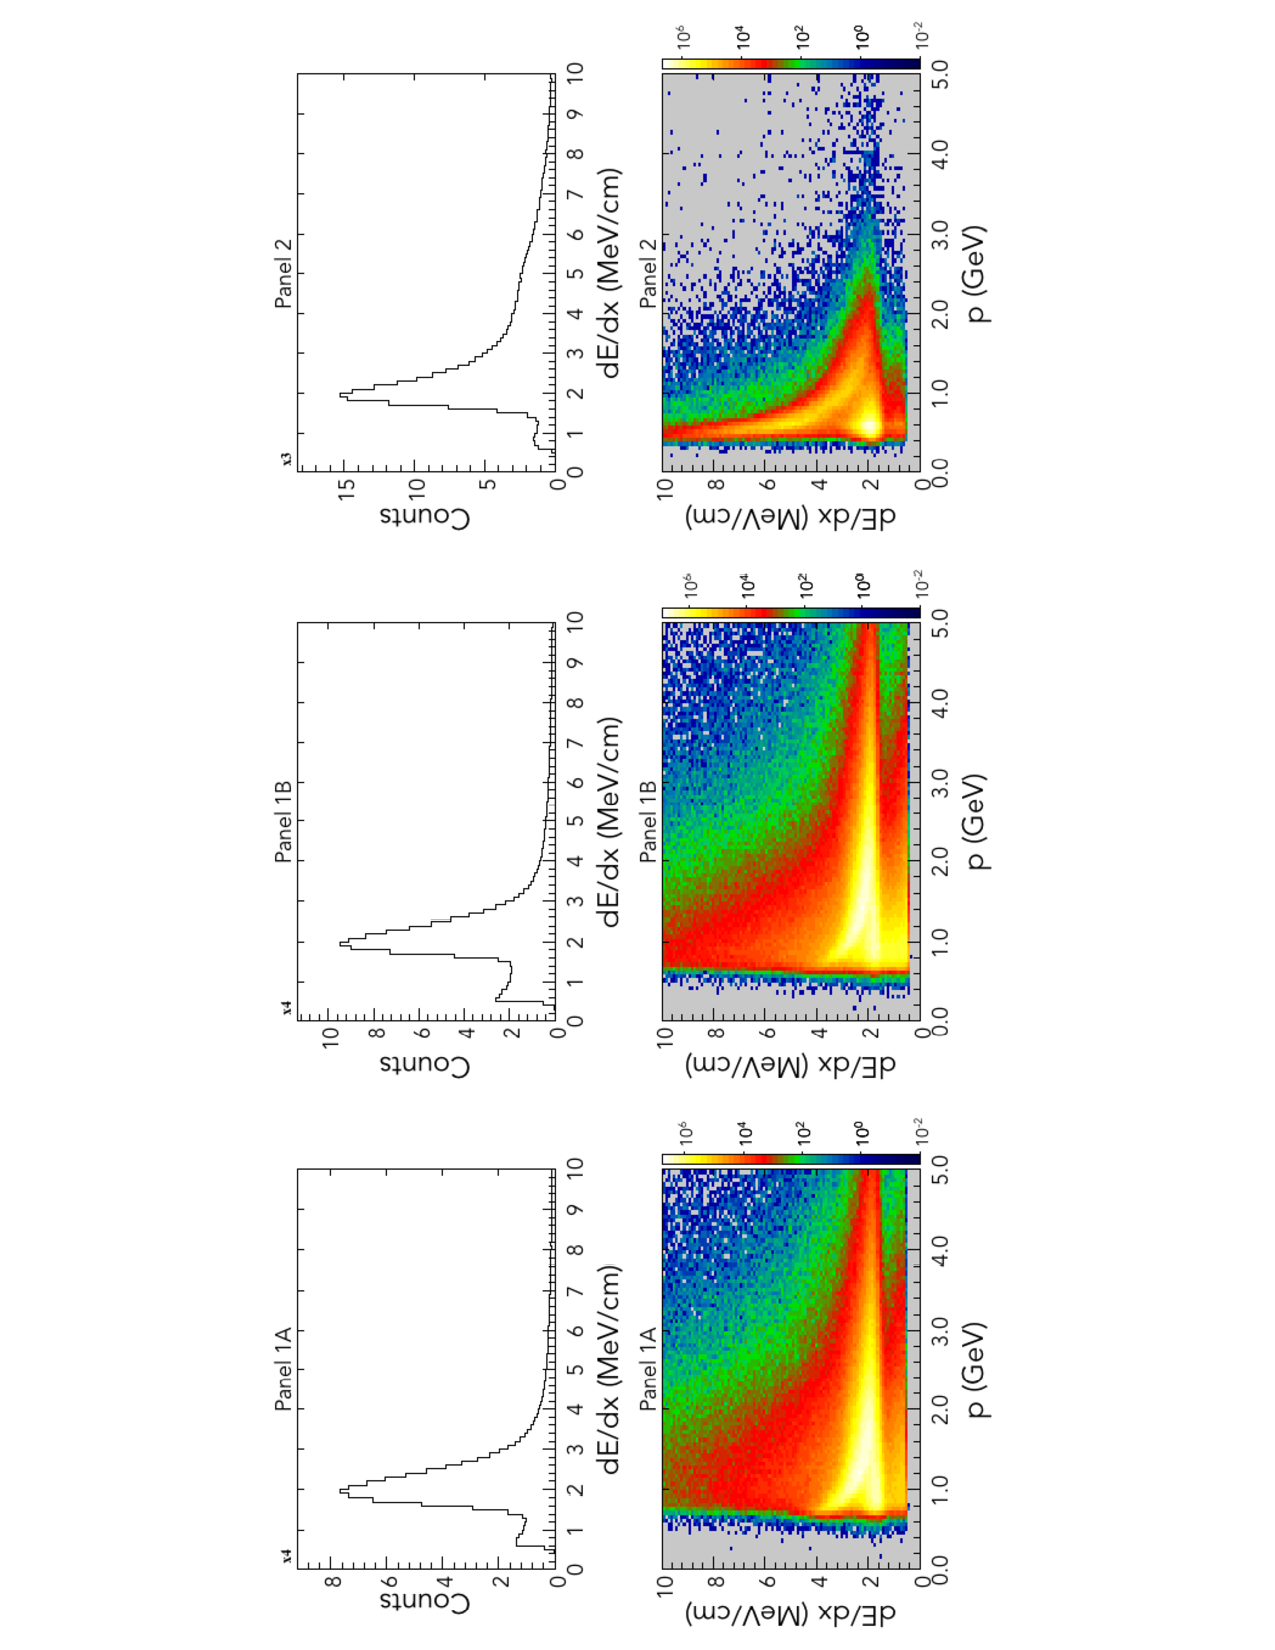
\includegraphics[width=0.52\textwidth,height=0.29\textheight,natwidth=610,natheight=642,angle=-90]
{pics/ftof-dedx.pdf}}}
\end{picture} 
\caption{Measured FTOF counter energy loss for positively charged particles from 10.6-GeV electrons
incident upon a liquid-hydrogen target normalized by the extrapolated path length from the projection
of the forward track through the counter array. The normalized $dE/dx$ (MeV/cm) spectrum shows
the separation of minimum-ionizing particles from more heavily ionizing particles summed over the
counters in panel-1a (left), panel-1b (middle), and panel-2 (left). The top row of plots show the normalized
$dE/dx$ and the bottom row of plots show $dE/dx$ vs. track momentum (GeV).}
\label{ftof-dedx}
\end{figure}
%%%%%%%%%%%%%%%%%%%%%%%%%%%%%%%%%%%%%%%%%%%%%%%%%%%%%%%%

\subsubsection{Attenuation Length Measurements}
\label{sec:attlen}

The measured ADC values for each PMT can be written in terms of the attenuation length as:

\begin{equation}
\label{al-adc}
(ADC - PED) = A_0 e^{-d/\lambda},
\end{equation}

\noindent
where $A_0$ is a constant, $d$ is the distance along the counter with respect to the PMT location, and
$\lambda$ is the counter attenuation length. Using the definition:

\begin{equation}
  d_{L/R} = \frac{L}{2} \pm coor,
\end{equation}

\noindent
where $L$ is the counter length, $coor$ is the FTOF hit coordinate along the bar (with the middle of the bar
at $coor=0$) defined as:

\begin{equation}
\label{coor}
coor = \frac{v_{eff}}{2} \cdot (t_L - t_R - C_{LR}),
\end{equation}

\noindent
$v_{eff}$ is the effective velocity of light in the scintillation bars (see Section~\ref{sec:veff} for details), and
$C_{LR}$ is the offset that centers the time difference distribution about 0.

The logarithmic ratio of the ADCs of the left and right PMTs from a given counter as a function of hit coordinate
along the bar can be written as:

\begin{equation}
\label{linear}
\log \left( \frac{(ADC-PED)_R}{(ADC-PED)_L} \right ) = C + \frac{2 \cdot coor}{\lambda}.
\end{equation}

\noindent
This expression can be used to determine the effective counter attenuation length using a linear fit of the
logarithmic ADC ratio vs. $coor$. The slope of this correlation is $2/\lambda$. In this expression, the
$y$-intercept $C$ is a constant given by $\log(A_0^R/A_0^L)$.

Figure~\ref{atten-len} shows the measured attenuation lengths for the FTOF counters in one sector of
the CLAS12 Forward Detector extracted from data with a 10.6~GeV electron beam incident upon a
liquid-hydrogen target.

%%%%%%%%%%%%%%%%%%%%%%%%%%%%%%%%%%%%%%%%%%%%%%%%%%%%%%%%%
\begin{figure}[htbp]
\vspace{1.2cm}
\begin{picture}(50,50) 
\put(-5,-45)
{\hbox{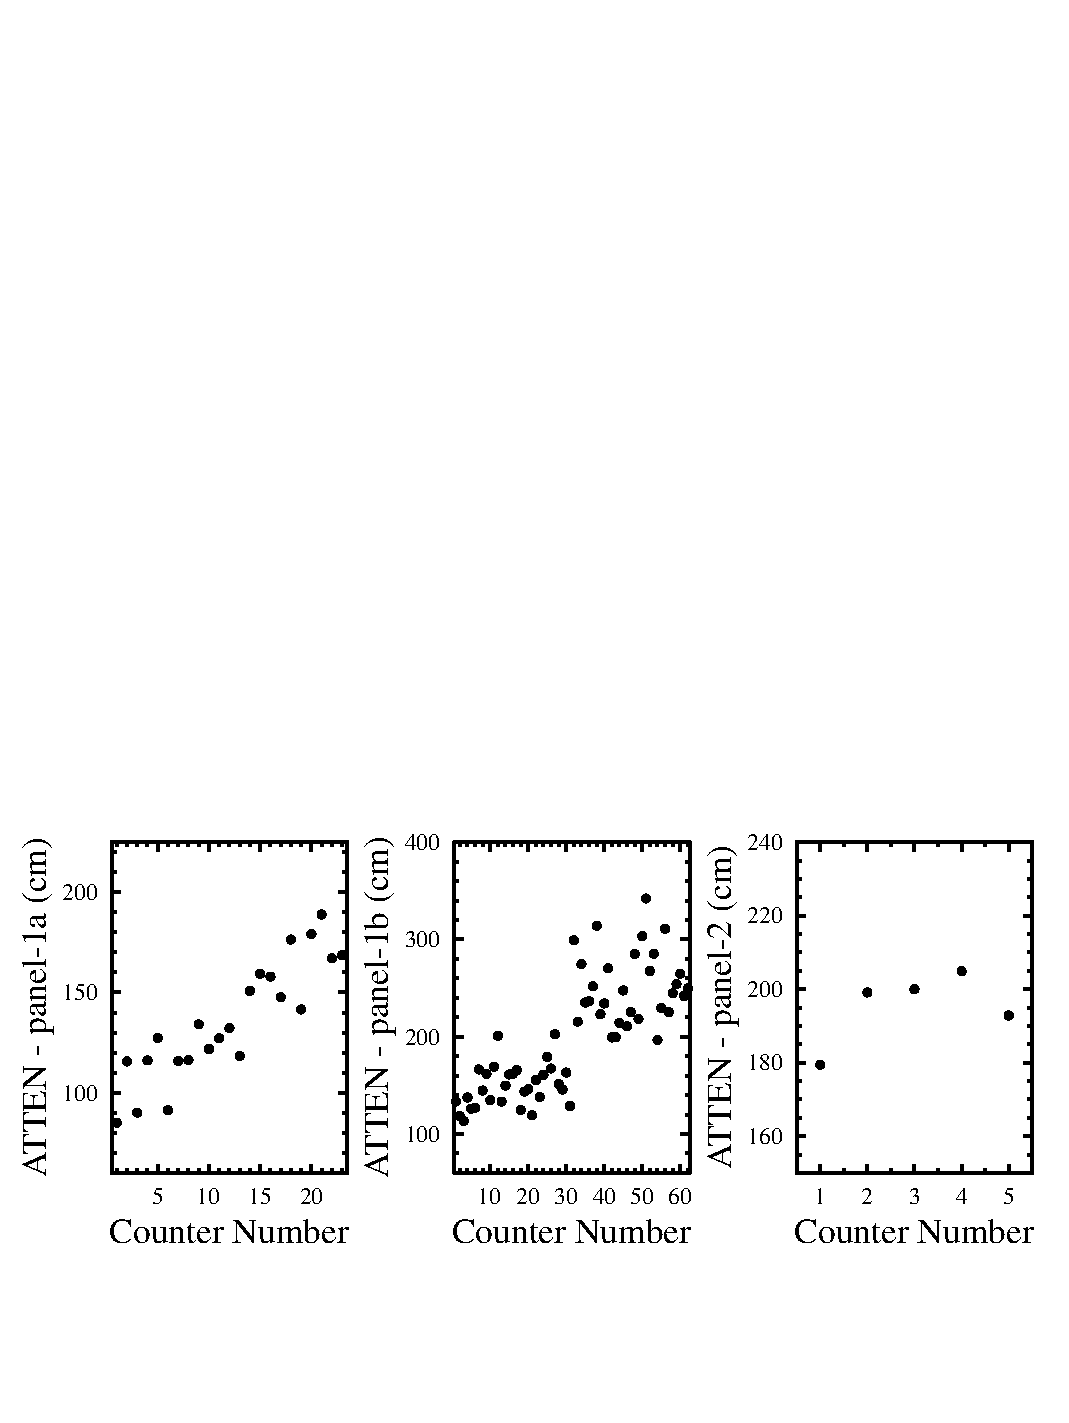
\includegraphics[width=0.59\textwidth,natwidth=610,natheight=642]{pics/atten-r4013.pdf}}}
\end{picture} 
\caption{Counter attenuation lengths (cm) vs. counter number for all FTOF counters in one sector of the
CLAS12 Forward Detector determined from beam data.}
\label{atten-len}
\end{figure}
%%%%%%%%%%%%%%%%%%%%%%%%%%%%%%%%%%%%%%%%%%%%%%%%%%%%%%%%%

\subsubsection{Effective Velocity Determination}
\label{sec:veff}

The effective velocity of light in each counter employs a calculation based on the comparison of the
reconstructed coordinate information along the scintillation bar from the left and right PMT TDC times
with the track hit coordinate determined from the extrapolation of the track beyond the drift chambers
to the location of the FTOF counters. Figure~\ref{veff} shows the measured effective velocity for each
counter in one sector of the CLAS12 Forward Detector using data with a 10.6-GeV electron beam incident
on a liquid-hydrogen target. 

As the counter length increases, so does $v_{eff}$ because more reflected light with smaller $v_{eff}$ is
lost due to attenuation along the bar compared to direct light with higher $v_{eff}$. The effective velocity
is used in the FTOF analysis to determine the hit time for each event from the measured TDC times. The
intrinsic position resolution is given by $v_{eff} \times \sigma(t_L - t_R)$ for each counter, which is
most relevant for the interactions of neutral particles. The position for charged particles at the location
of the FTOF counters can be measured more precisely with the forward tracking system (the track hit
coordinate resolution at the FTOF counters is 1-2~cm, while the FTOF hit coordinate resolution is 1-4~cm,
depending on the counter timing resolution). However, the hit coordinate of charged particles along the length
of the FTOF counters determined from FTOF information alone (see Eq.(\ref{coor})) can be compared to that
from forward tracking projected to the FTOF location to ensure the FTOF hits are properly matched to the
tracks.

%%%%%%%%%%%%%%%%%%%%%%%%%%%%%%%%%%%%%%%%%%%%%%%%%%%%%%%%%
\begin{figure}[htbp]
\vspace{1.3cm}
\begin{picture}(50,50) 
\put(-5,-45)
{\hbox{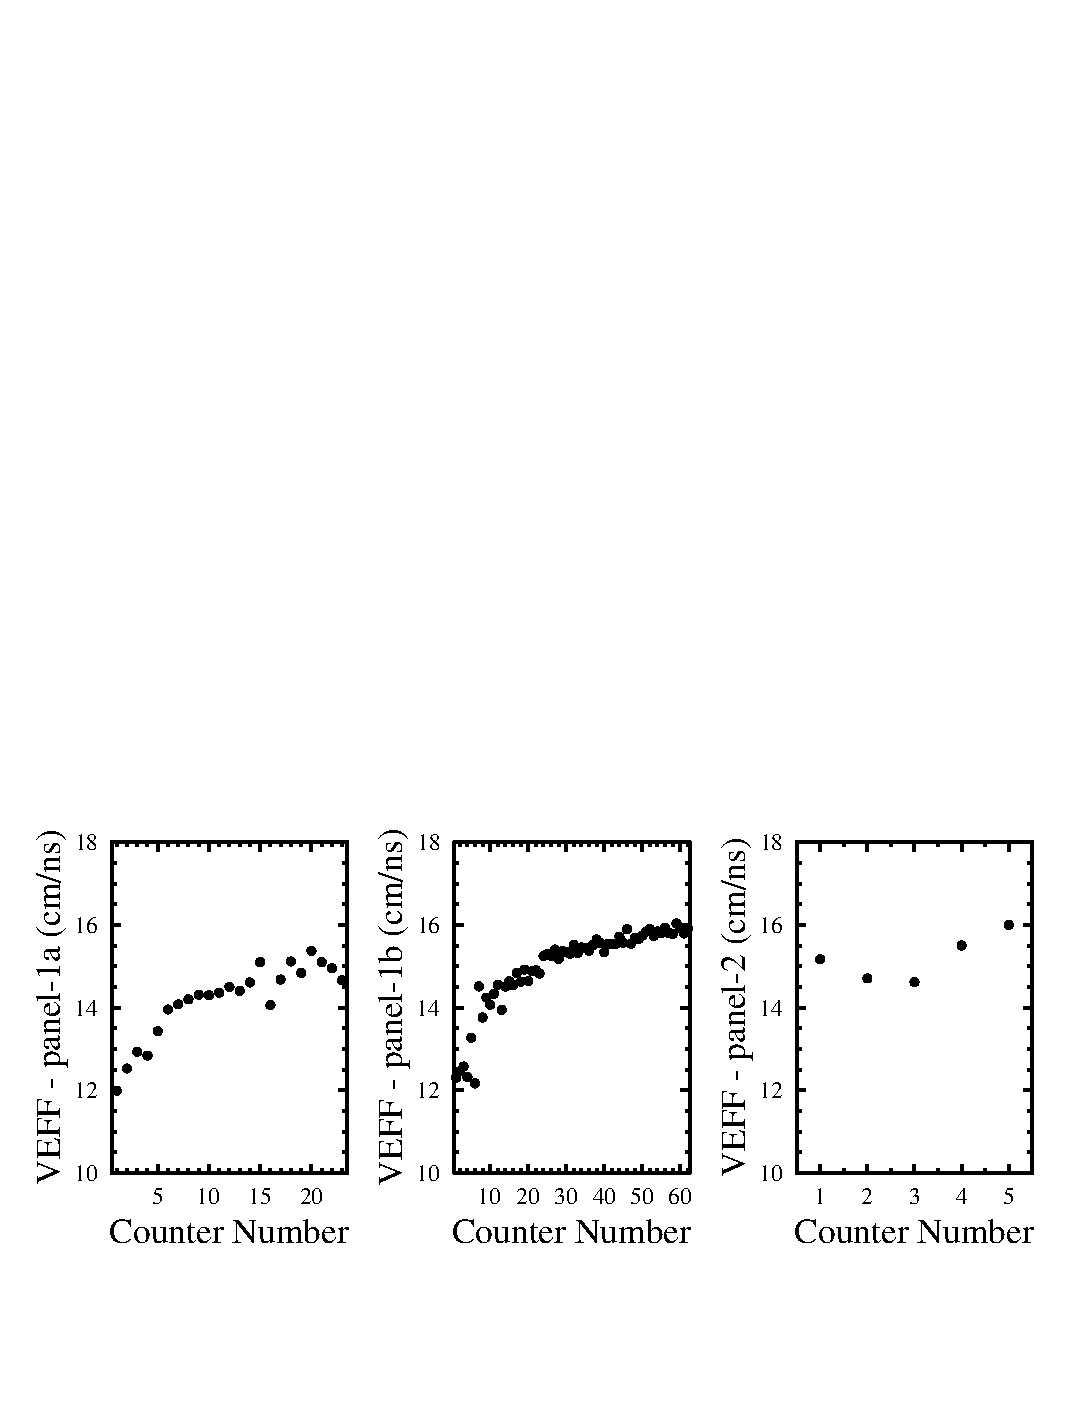
\includegraphics[width=0.59\textwidth,natwidth=610,natheight=642]{pics/veff-r4013.pdf}}}
\end{picture} 
\caption{Counter effective velocities (cm/ns) vs. counter number for all FTOF counters in one sector of
the CLAS12 Forward Carriage determined from beam data.}
\label{veff}
\end{figure}
%%%%%%%%%%%%%%%%%%%%%%%%%%%%%%%%%%%%%%%%%%%%%%%%%%%%%%%%%

\subsubsection{Time-Walk Corrections}
\label{sec-tw}

The approach that we have adopted to correct the FTOF TDC times for time-walk effects is different from
the one employed for our bench test studies of the counters in their cosmic ray test stands described in
Section~\ref{sec-bench}. We ultimately settled on an approach that first accounts for an average hit
position-independent correction (called TW in Fig.~\ref{calib-seq}) with a time-walk functional of a
power-law form:

\begin{equation}
\label{tw-func}
t^{corr}_{L,R} = t_{L,R} - \frac{tw0_{L,R}}{\sqrt{(ADC - PED)_{L,R}}}.
\end{equation}

The time-walk amplitude parameters $tw0_{L,R}$ are determined by defining the following vertex time
residuals for each PMT:

\begin{equation}
\label{tres}
t_{L,R}^{res} = \left(t_{L,R} - \frac{d_{L,R}^{FT}}{v_{eff}} - \frac{P_L}{\beta c} \right) 
- \left( t_{RF} + \frac{z_{vert}}{\beta_e c} \right),
\end{equation}

\noindent
where $t_{L,R}$ are the measured TDC times after the left/right PMT time offset correction, $d^{FT}/v_{eff}$
corrects the time measured at the PMT to the time at the track hit point on the counter determined from the
forward tracking information, and $P_L/(\beta c)$ is the track flight time from the reaction vertex to the
FTOF. The track path length $P_L$ and $\beta$ are defined via forward tracking and the particle identification
is determined from the Event Builder~\cite{daq-nim}. The term $z_{vert}/(\beta_e c)$ corrects the RF time
$t_{RF}$ for the actual electron beam event vertex location along the $z$-axis of the extended target. This
vertex time residual represents the FTOF hit time from a single PMT traced back to the reaction vertex and
compared to a precise time reference $t_{RF}$ given by the RF signal from the accelerator. As $t_{RF}$
represents a reference time for the arrival of the electron beam bunch at a fixed position along the beamline in
Hall~B assigned as the center of the target, the time must be corrected for the displacement of the reaction
vertex along the extended length of the target.

As the beam bucket that was associated with the event is not determined at this point, the time walk for each
PMT is actually determined using the modulus of $t^{res}_{L,R}$ with the RF beam bucket period
$T_{RF}=$1/(RF frequency) by fitting:

\begin{equation}
t'_{L,R} = mod \left[t^{res}_{L,R}, T_{RF}\right]~{\rm vs.}~(ADC-PED)_{L,R}.
\end{equation}

Figure~\ref{twalk-plot} shows the $t'$ vs. $ADC$ distribution for a representative FTOF PMT in
panel-1b from beam data using a 10.6-GeV electron beam incident upon a 5-cm long liquid-hydrogen
target. Note that all distributions that employ $t'_{L,R}$ are sorted in 25~ps bins (consistent with
the TDC LSB). The overall scale of the time-walk effects spanning the full dynamic range of the
ADC is 2~ns.

%%%%%%%%%%%%%%%%%%%%%%%%%%%%%%%%%%%%%%%%%%%%%%%%%%%%%%%%%%
\begin{figure}[htbp]
\vspace{2.0cm}
\begin{picture}(50,50) 
\put(20,-70)
{\hbox{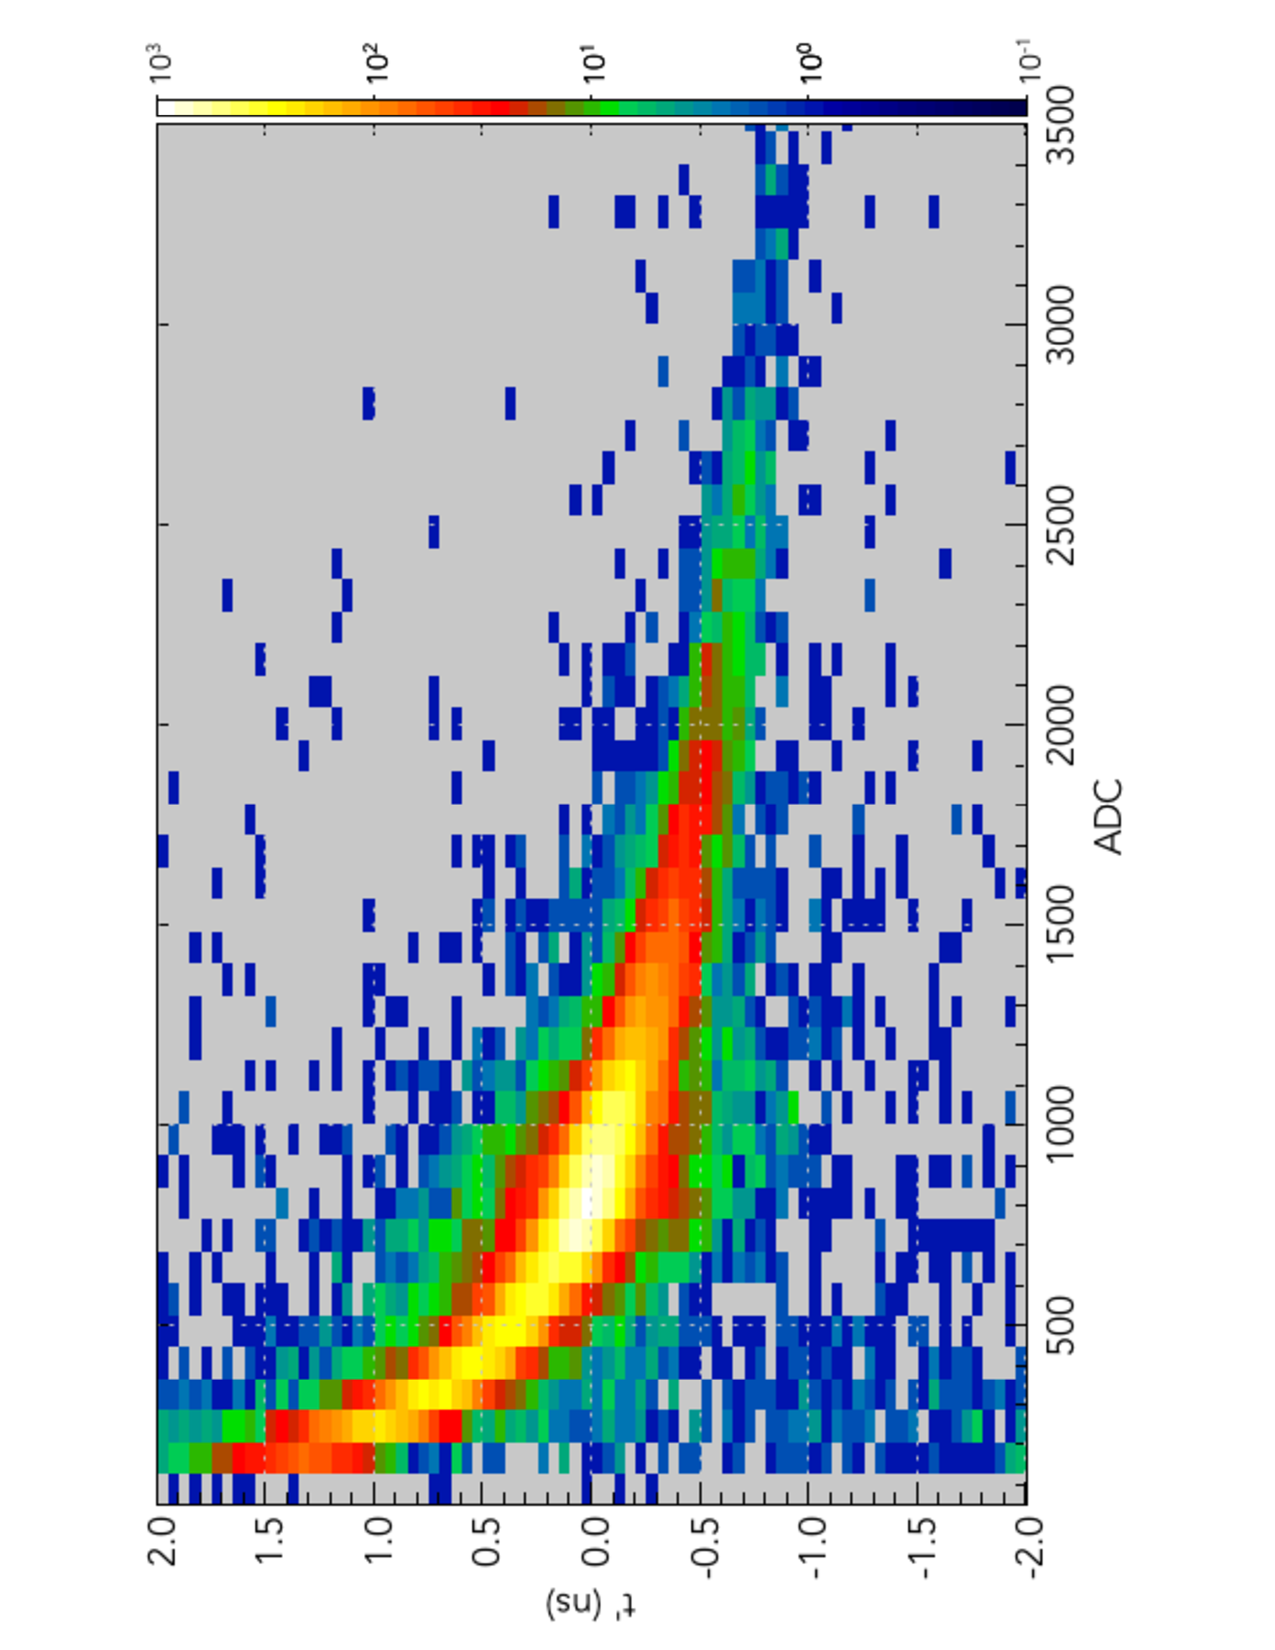
\includegraphics[width=0.40\textwidth,natwidth=610,natheight=642]{pics/twalk-plot.pdf}}}
\end{picture} 
\caption{Plot of $t'$ (ns) vs. $ADC$ for one representative left PMT from panel-1b from beam data. As
$t'$ is defined using the modulus of $T_{RF}$, its limits span $\pm T_{RF}/2$. The overlaid curve
represents the time-walk functional fit from Eq.(\ref{tw-func}).}
\label{twalk-plot}
\end{figure}
%%%%%%%%%%%%%%%%%%%%%%%%%%%%%%%%%%%%%%%%%%%%%%%%%%%%%%%%%%

The second part of the full time-walk correction accounts for additional position-dependent effects as
discussed in Section~\ref{sec-bench} (called TWP in Fig.~\ref{calib-seq}) . After the position-independent
time-walk correction is determined, in a second step we then fit a second-order polynomial to the counter hit time
vs. hit position along the counter defined from the projection of the charged particle track on the FTOF from
the forward tracking system. The time employed for this step is the track hit time at the vertex (relative
to the vertex-corrected RF time) averaging the left and right PMT hit times (see definition in
Section~\ref{sec-talign}). Figure~\ref{twalk-pos} shows the distribution before and after the second correction.
The before distribution where only the position-independent time-walk correction is applied, reveals a
characteristic ``smile'' pattern, which reflects the unaccounted for position-dependent time-walk effects on
the measured times incorporating both the left and right PMTs each with their own linearly falling time-walk
parameters when moving away from each PMT as discussed in Section~\ref{sec-bench}. Effectively this approach
actually accounts for all remaining position dependences in the calibration parameters. Specifically, it also takes
care of the effective velocity changes with position along the bar moving away from the PMT. However, the
dominant position-dependence accounted for here is related to the time-walk.

%%%%%%%%%%%%%%%%%%%%%%%%%%%%%%%%%%%%%%%%%%%%%%%%%%%%%%%%%%
\begin{figure}[htbp]
\vspace{5.7cm}
\begin{picture}(50,50) 
\put(20,45)
{\hbox{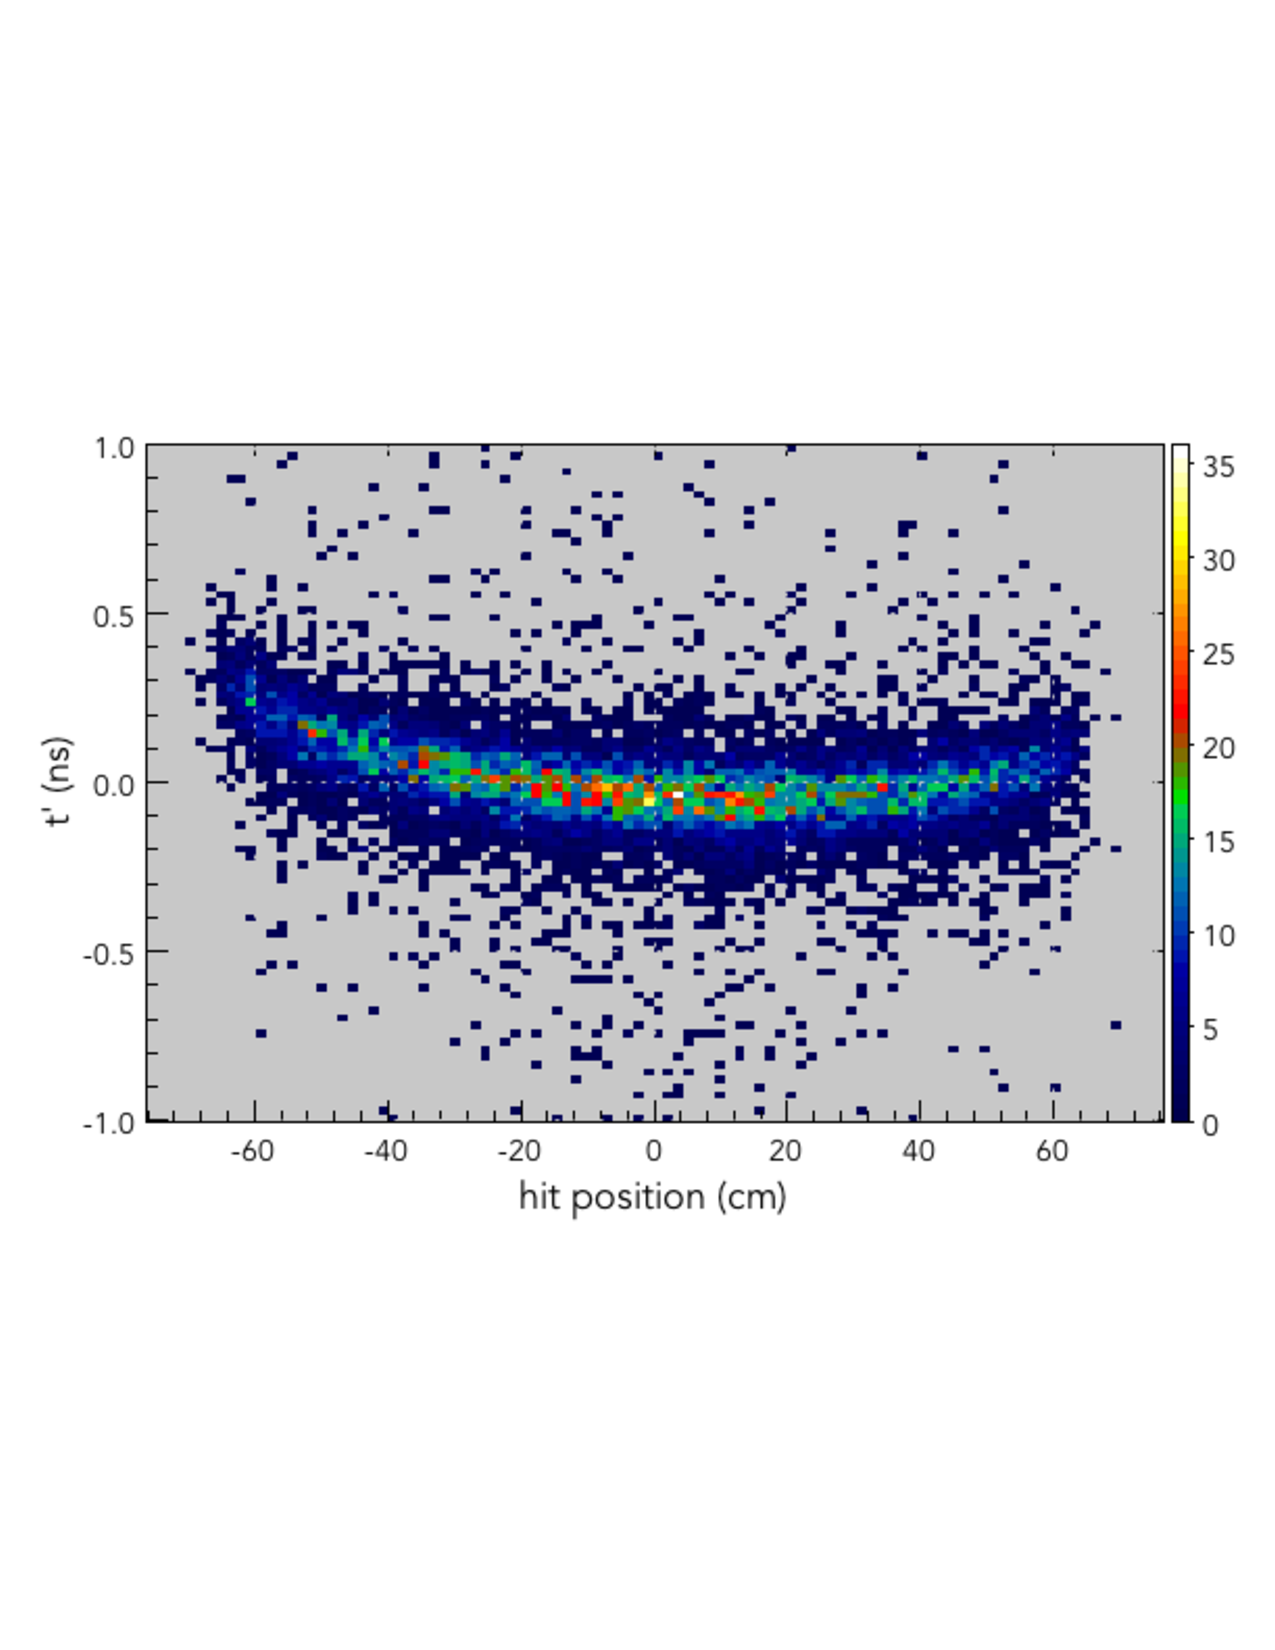
\includegraphics[width=0.38\textwidth,natwidth=610,natheight=642]{pics/p1b-posdep1.pdf}}}
\put(20,-70)
{\hbox{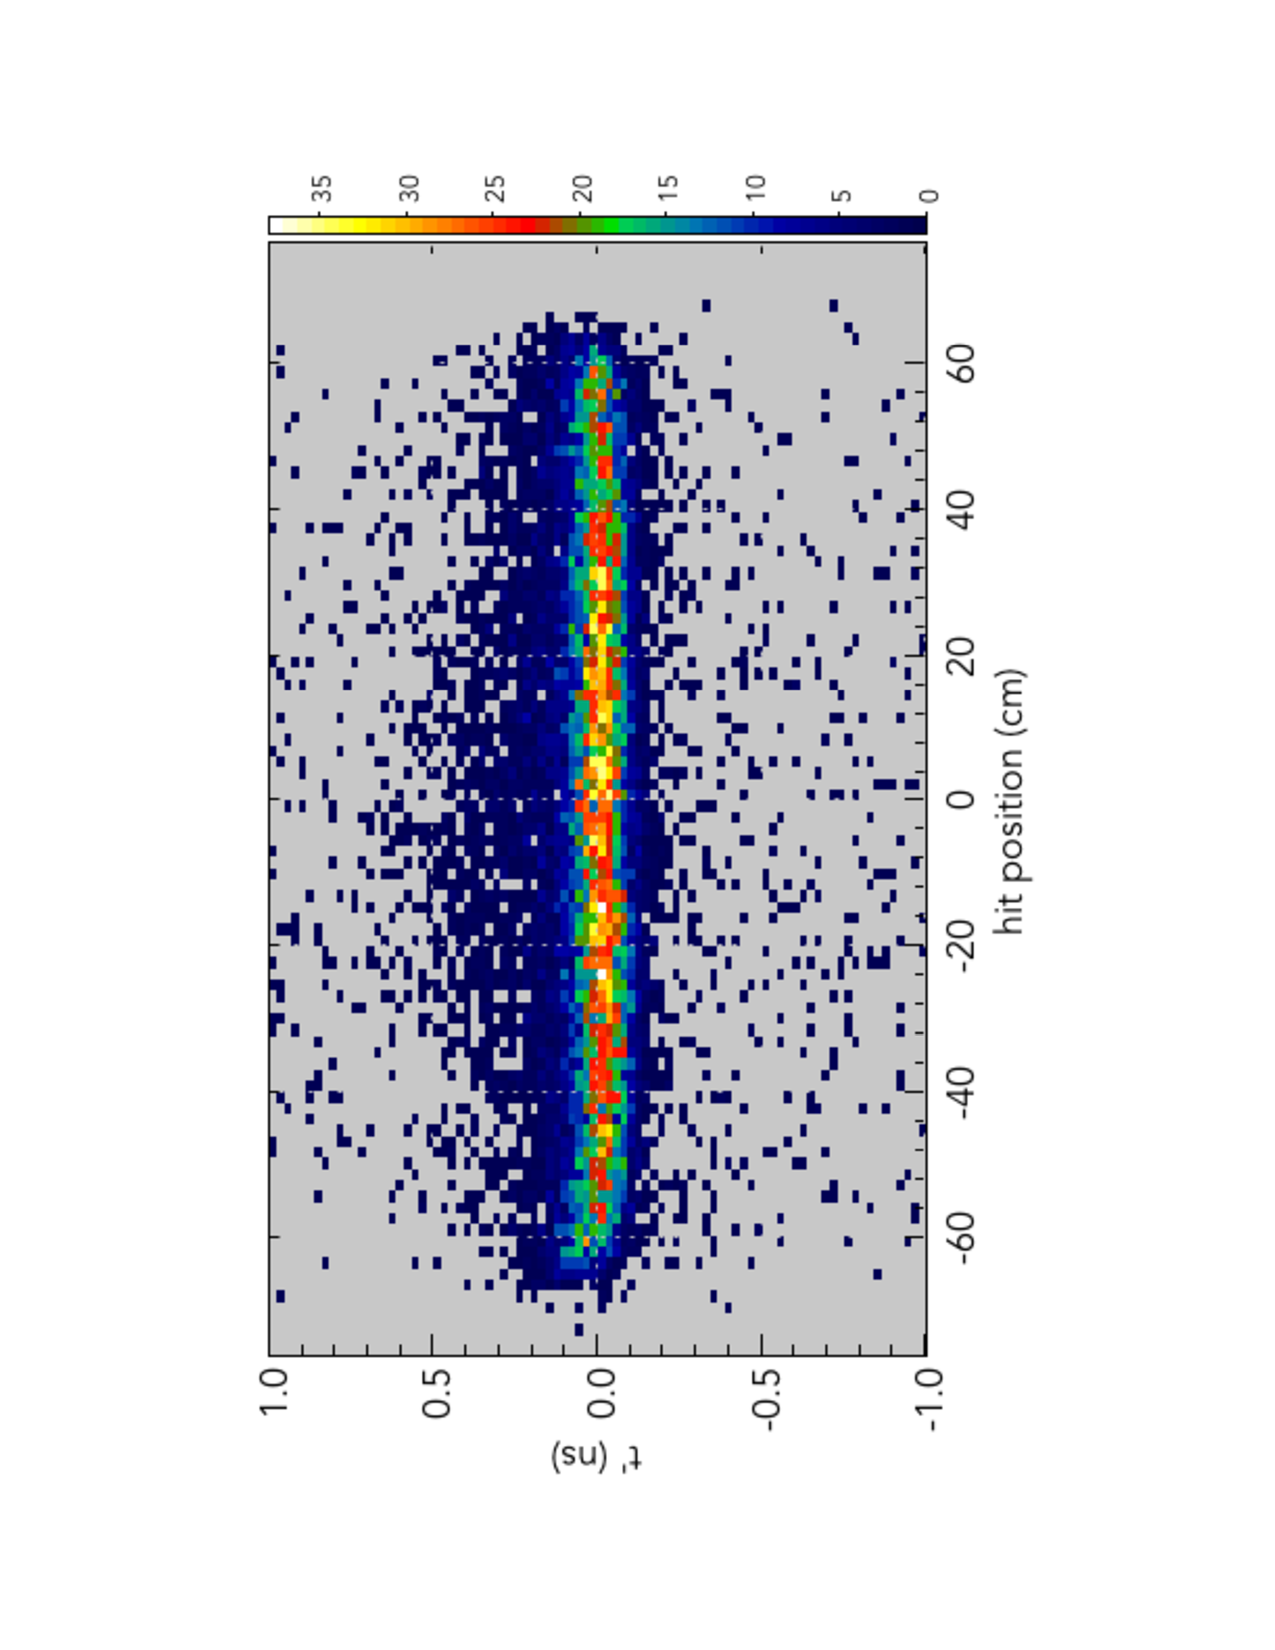
\includegraphics[width=0.38\textwidth,natwidth=610,natheight=642]{pics/p1b-posdep2.pdf}}}
\end{picture} 
\caption{Plot of $t'$ (ns) vs. hit position (cm) along the bar from beam data after the
position-independent time-walk correction (top) and after the ad hoc second-order polynomial correction
to remove the residual coordinate dependence (bottom).}
\label{twalk-pos}
\end{figure}
%%%%%%%%%%%%%%%%%%%%%%%%%%%%%%%%%%%%%%%%%%%%%%%%%%%%%%%%%%

Note that the RFP fine-timing calibration step (see Section~\ref{sec-talign}) is completed three separate
times in the calibration sequence. The first time is to center the vertex time distributions in the $T_{RF}$
window to avoid wrap-around in the RF period range when taking the modulus of the vertex time difference
with the RF time. The RFP calibration step is repeated after the second LR step due to shifts of the left
and right PMT times and before the position-dependent time-walk calibration (TWP). A final RFP calibration
is carried out to account for the vertex time shifts that result from the position-dependent time-walk
corrections.

\subsubsection{Counter-to-Counter Time Alignment}
\label{sec-talign}

The flight time of a charged particle from the reaction vertex to an FTOF counter is given by:

\begin{equation}
t_p = \overline{t}_{hit} - t_{ST},
\end{equation}

\noindent
where $\overline{t}_{hit}$ is the average FTOF counter hit time from the left and right PMTs (see
Section~\ref{cluster}) and $t_{ST}$ is the event start time. The event start time is associated with the
RF but needs to be synchronized with the particular RF beam bucket associated with the event. The
beam bunch width within the RF beam bucket is only about 2~ps and, therefore, represents a precise time
marker. However, as the RF time signal has a period of $T_{RF}$, it is not a priori known which RF beam
bucket is the one associated with the event that led to the hit in the FTOF counter.

The determination of the absolute flight time of charged particle tracks from the reaction vertex to an
FTOF counter is performed in two steps. In the first step (called RFP in Fig.~\ref{calib-seq}), fine timing
offsets (binned in the 25~ps TDC LSB) are determined to align the FTOF hit times traced back to the
reaction vertex for each counter within the RF time window. In the second step (called P2P in
Fig.~\ref{calib-seq}), coarse timing offsets binned in units of the RF period $T_{RF}$ are determined to
select the specific RF beam bucket associated with the event.

The fine timing alignment algorithm uses the FTOF hit time traced back to the event vertex relative
to the RF to align the vertex times of all FTOF hits (modulo $T_{RF}$). However, instead of using the
separate left and right PMT hit times as in Eq.(\ref{tres}), this algorithm uses the average counter
hit times, 
\begin{eqnarray}
t_{res}' = mod \left[ t_{vtx}, T_{RF} \right], ~~~~~\\ [1ex]
t_{vtx} = \left(\overline{t}_{hit} - \frac{P_L}{\beta c} \right) - 
\left(t_{RF} + \frac{z_{vert}}{\beta_e c} \right). \nonumber
\end{eqnarray}

Figure~\ref{rfp-plot} shows the $t_{res}'$ distribution for one representative FTOF counter. The
centroid of the Gaussian fit gives the fine timing offset. The width of the Gaussian fit is a measure
of the effective time resolution of the counter. To display the full $t_{res}'$ distribution avoiding any
wrap-around effects near the edges of the $T_{RF}$ range, the algorithm plots the $t_{res}'$ distribution
in a range of $\pm T_{RF}/2$ about the peak channel in the distribution.

%%%%%%%%%%%%%%%%%%%%%%%%%%%%%%%%%%%%%%%%%%%%%%%%%%%%%%%%%%
\begin{figure}[htbp]
\vspace{1.7cm}
\begin{picture}(50,50) 
\put(0,135)
{\hbox{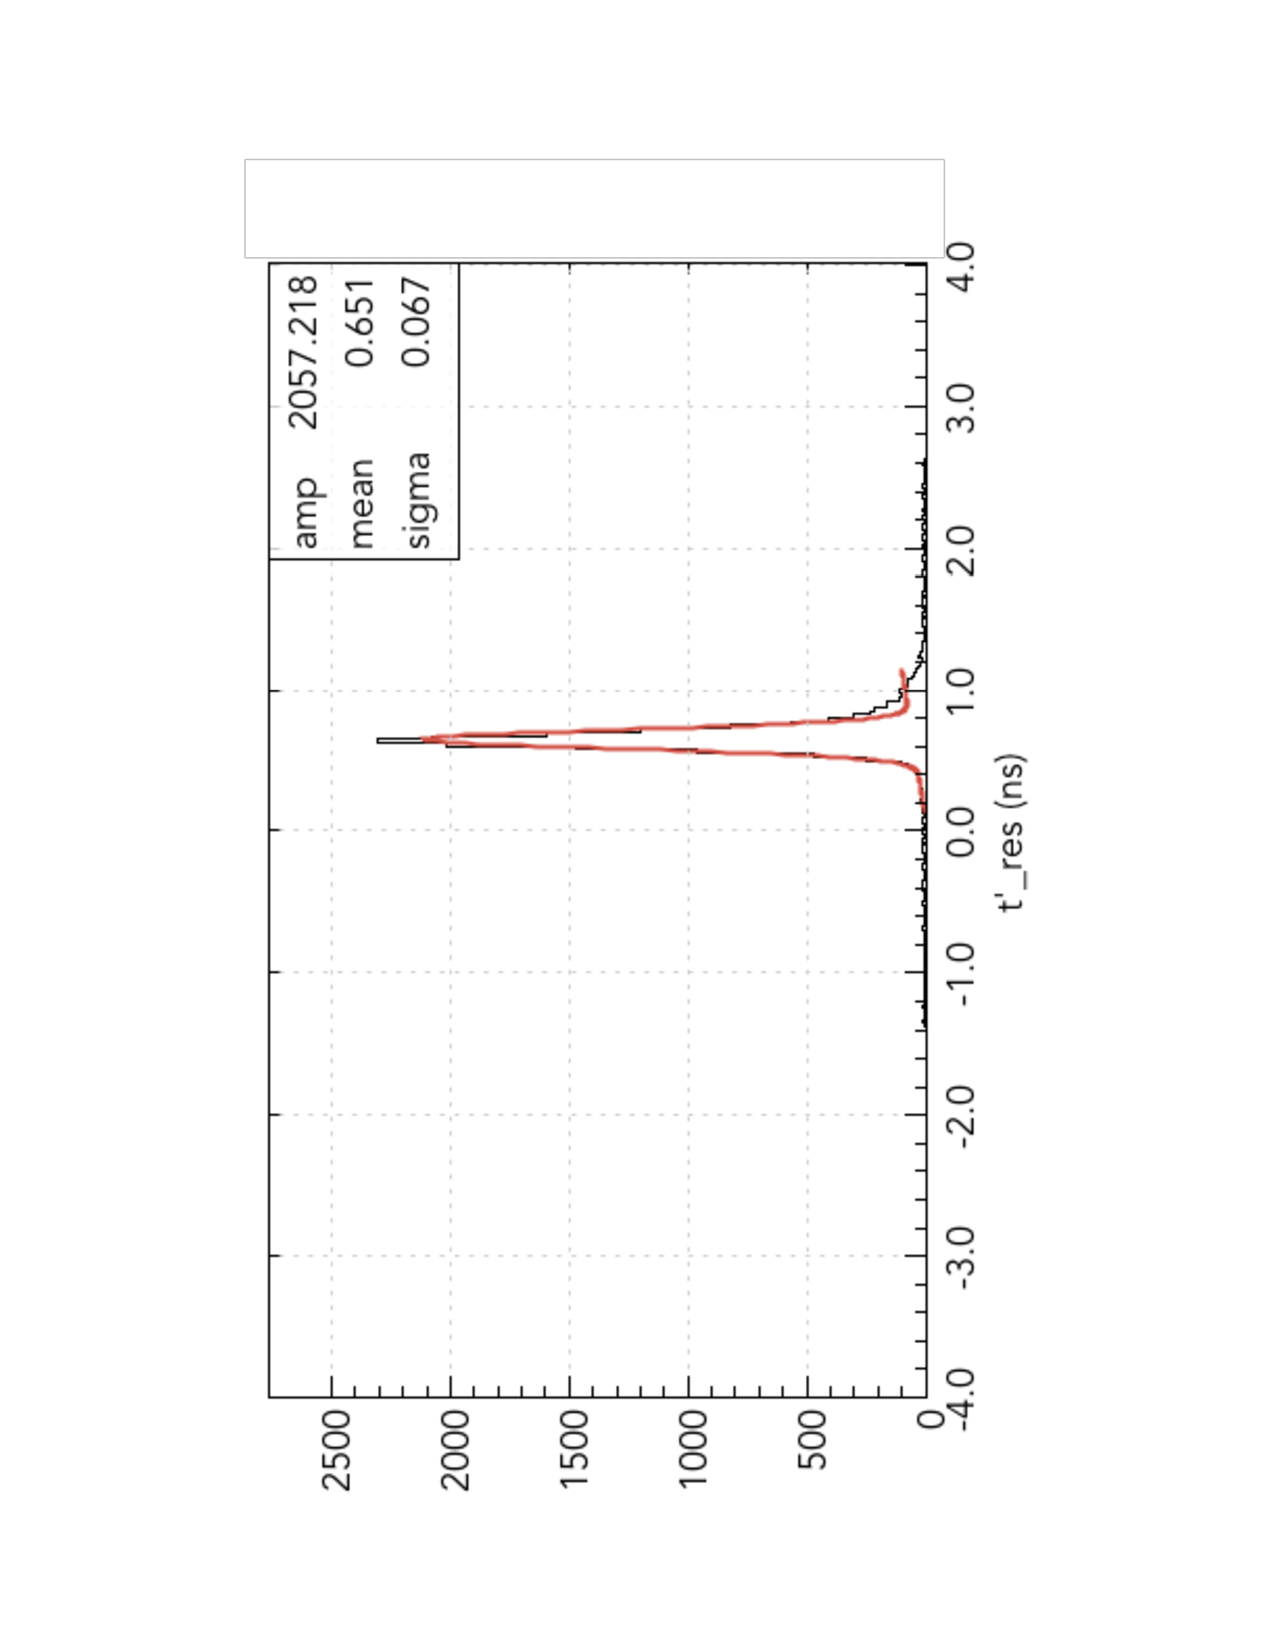
\includegraphics[width=0.38\textwidth,natwidth=610,natheight=642,angle=-90]{pics/rfp-plot.pdf}}}
\end{picture} 
\caption{Distribution of the FTOF hit times from beam data traced back to the vertex relative to the RF
(ns) for one representative FTOF panel-1b counter with the Gaussian plus background fit overlaid to
determine the counter RF offset and the effective counter time resolution. As $t'_{res}$ is defined using
the modulus of $T_{RF}$, this distribution is limited to span $\pm T_{RF}/2$ about the peak centroid.}
\label{rfp-plot}
\end{figure}
%%%%%%%%%%%%%%%%%%%%%%%%%%%%%%%%%%%%%%%%%%%%%%%%%%%%%%%%%%

After the fine timing offset calibration, the counter timing is precisely aligned modulo $T_{RF}$. The next
step in the FTOF timing calibration is to fix the measured hit times for all counters to the specific RF bunch
associated with the event.  This is carried out using coincidences of charged particle tracks to link the hit
times of all counters across the full FTOF system.

The coarse timing offset algorithm (called P2P for paddle-to-paddle) selects events with two forward-going
charged tracks and computes the vertex time difference between any given FTOF counter relative to hits in
all of the other FTOF counters,

\begin{equation}
t_{P2P} = t_{vert}^1 - t_{vert}^2,
\end{equation}

\noindent
where,

\begin{equation}
t_{vert}^i = \overline{t}_{hit}^i - \frac{P_L}{\beta c}.
\end{equation}

At this point the counter timing has already been aligned to within a multiple of $T_{RF}$. Note that
particle identification of each track is given by the Event Builder~\cite{daq-nim}, and as both tracks are
assumed to originate from the same reaction vertex, no vertex time corrections are necessary. The
algorithm adjusts the vertex time differences between all counters to zero. The coarse time offsets
represents a single parameter for each counter that is restricted to values of $n \cdot T_{RF}$, with
$n = 0, \pm 1, \pm 2, ...$.

Figure~\ref{p2p-plot} shows the $t_{P2P}$ distribution for one representative FTOF counter before and
after the coarse timing alignment. As expected, the final histogram is dominated by events in a single channel
(of width $T_{RF}$) centered at $T_{RF} = 0$. As these constants are predominantly determined by the
fixed system cable lengths, of which there are four different lengths used to connect the panel-1a and the
panel-1b counters, the constants primarily reflect the differences in the signal propagation times along
the signal cables. Note that the algorithm specifically identifies two track events for the calibration and
does not consider hits in panel-1b and panel-1a associated with the same track.

%%%%%%%%%%%%%%%%%%%%%%%%%%%%%%%%%%%%%%%%%%%%%%%%%%%%%%%%%%
\begin{figure}[htbp]
\vspace{1.9cm}
\begin{picture}(50,50) 
\put(0,-65)
{\hbox{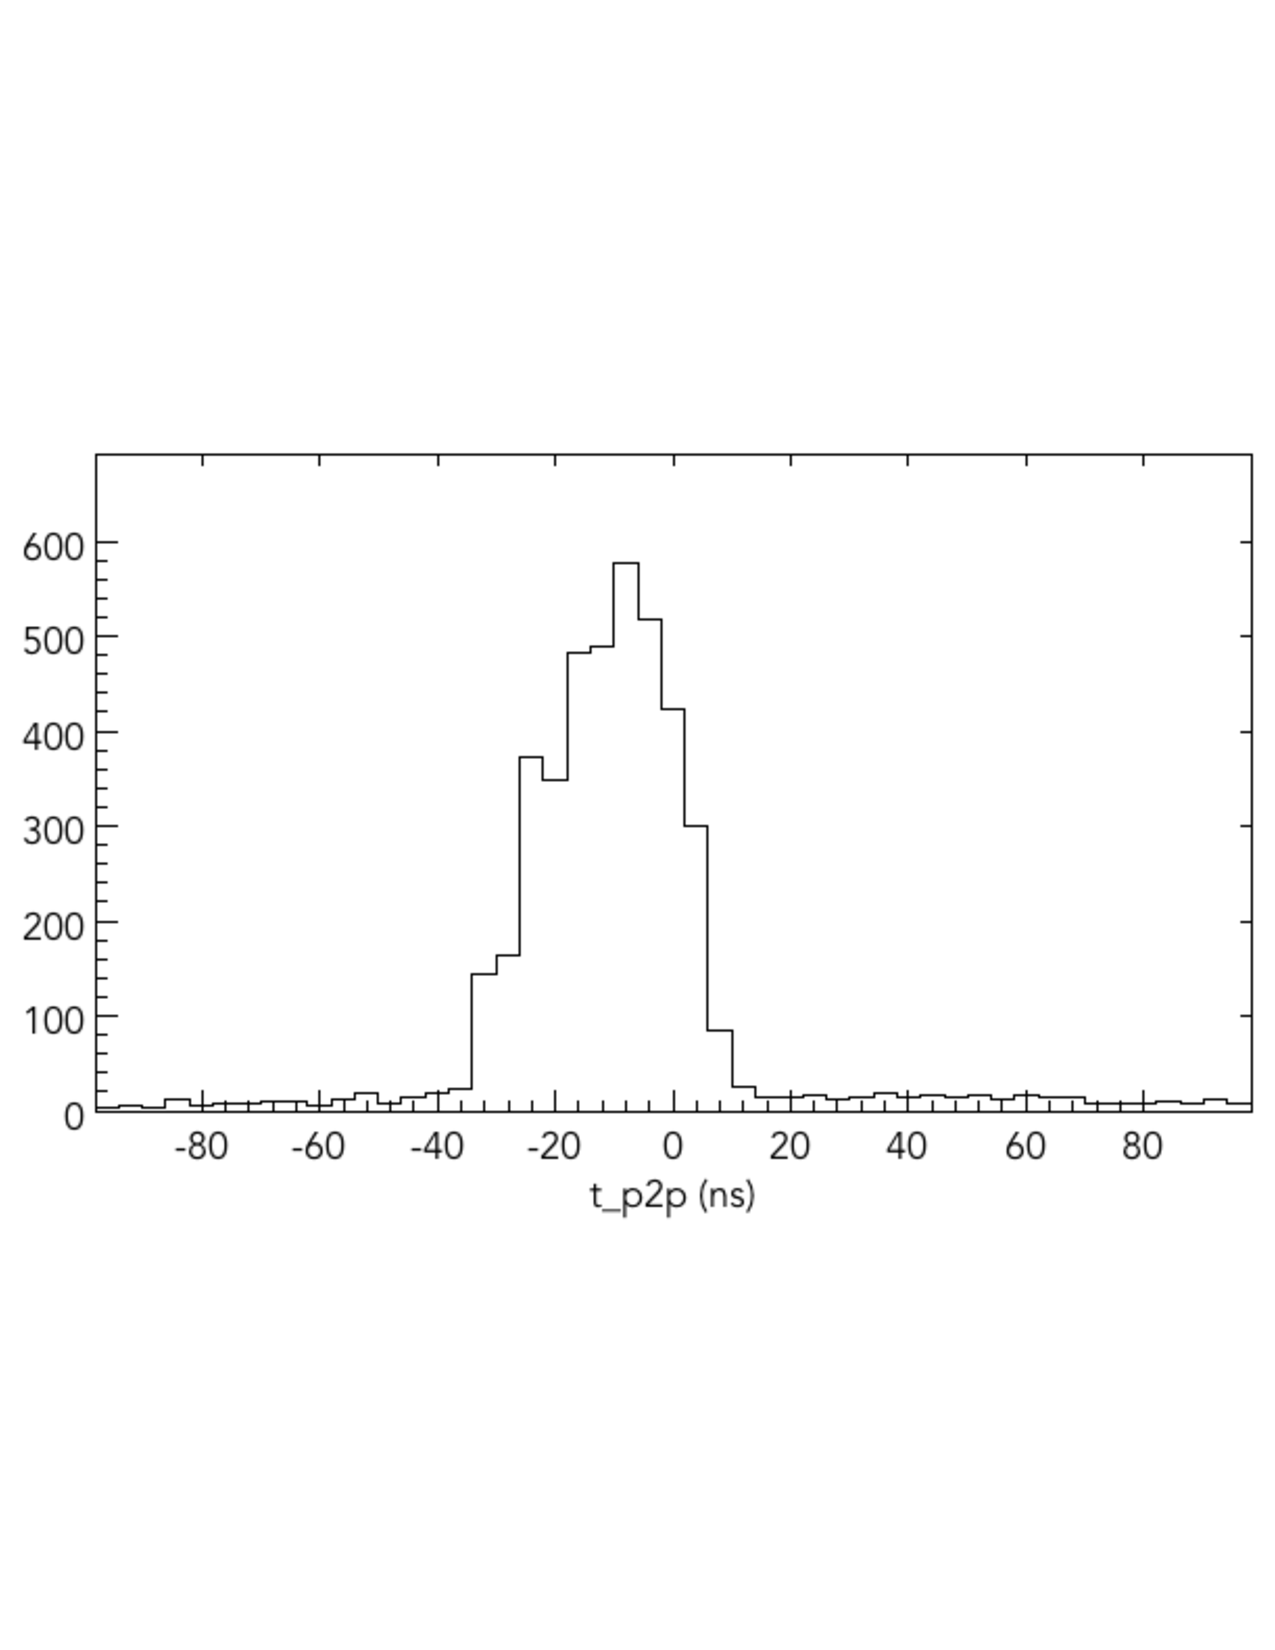
\includegraphics[width=0.23\textwidth,height=0.29\textheight,natwidth=610,natheight=642]
{pics/p2p-plot1.pdf}}}
\put(115,-65)
{\hbox{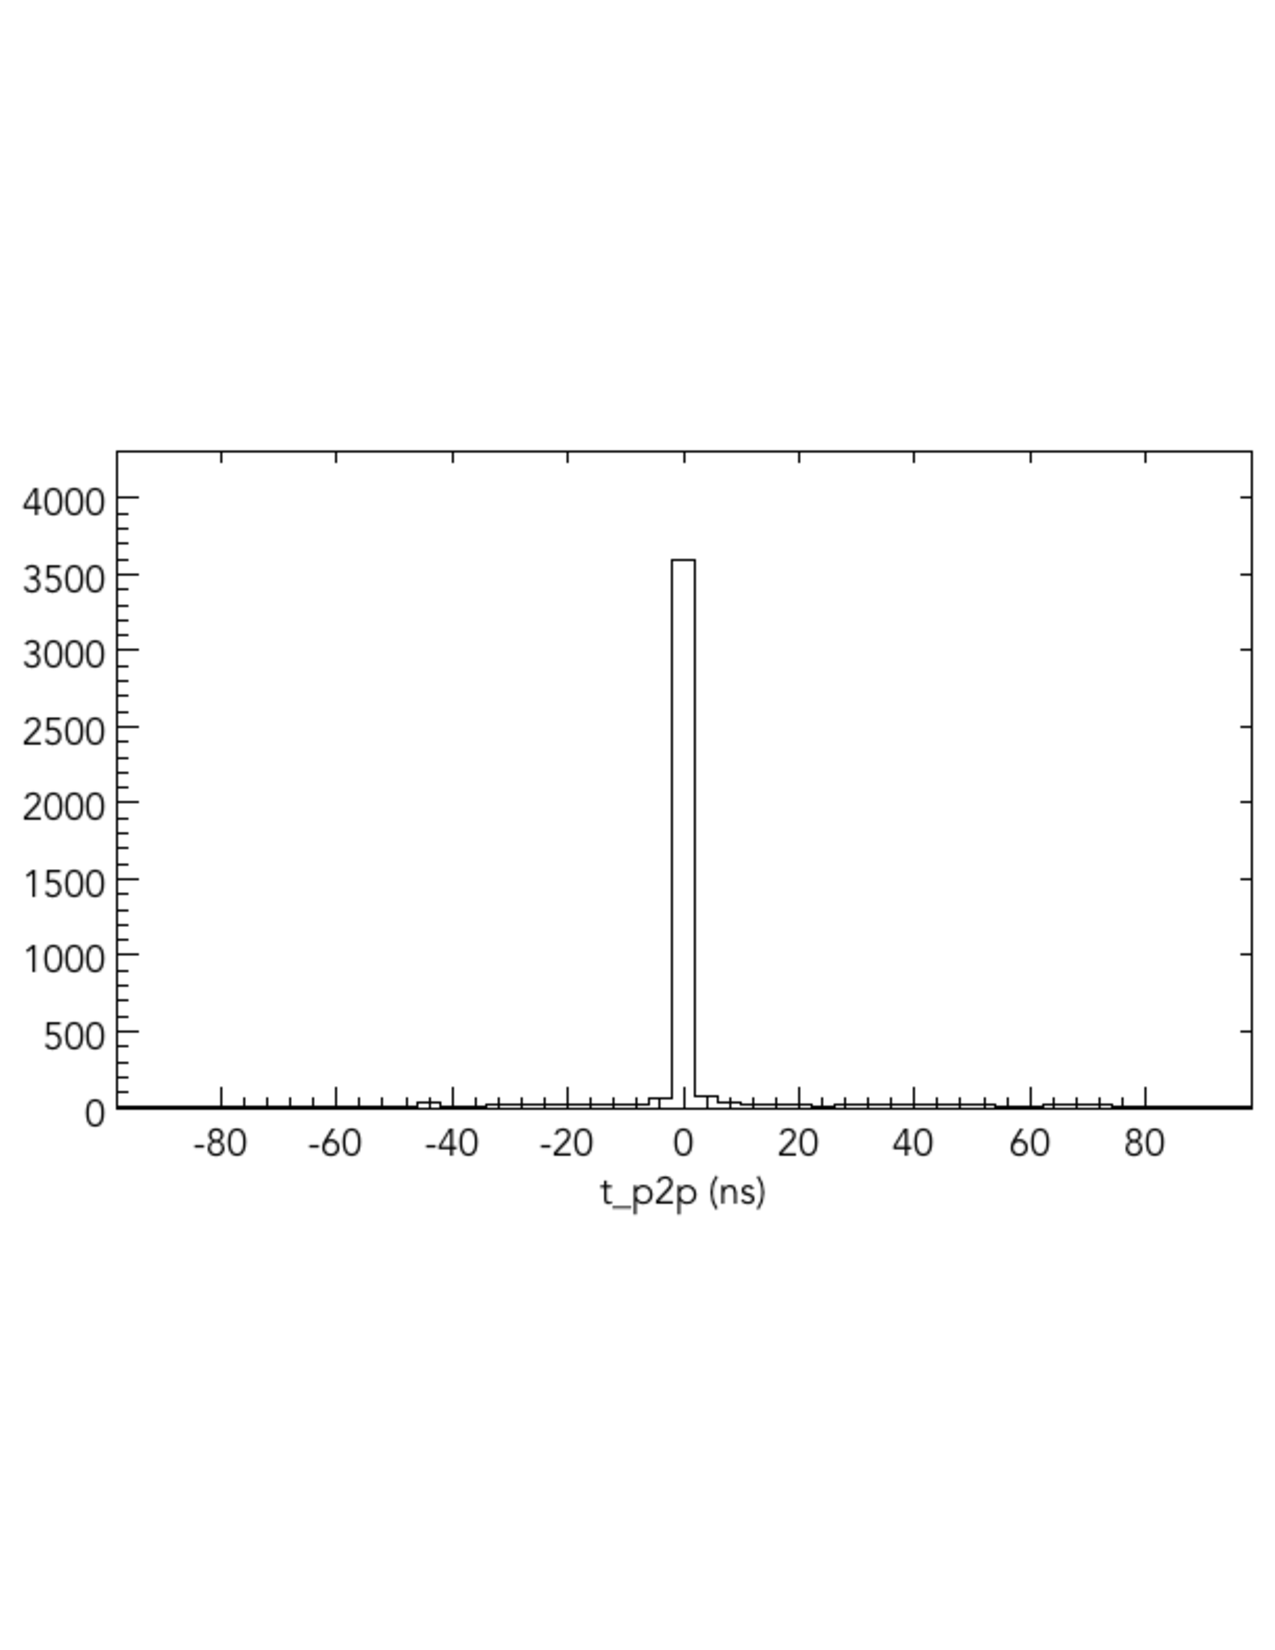
\includegraphics[width=0.23\textwidth,height=0.29\textheight,natwidth=610,natheight=642]
{pics/p2p-plot2.pdf}}}
\end{picture} 
\caption{Distribution of the vertex time differences (ns) for tracks in a single representative FTOF
counter compared to tracks in all other FTOF counters using event samples with two forward-going
charged particle tracks. (Left) Before P2P corrections and (right) after P2P corrections. The histogram
is sorted in bins of $T_{RF}$.}
\label{p2p-plot}
\end{figure}
%%%%%%%%%%%%%%%%%%%%%%%%%%%%%%%%%%%%%%%%%%%%%%%%%%%%%%%%%%

\subsubsection{TDC Calibration}
\label{sec-tdccal}

The calibration sequence also allows for calibration of the TDCs. This calibration is a single constant for
each TDC input channel in the system that converts the measured TDC digitization bin into time. The nominal
TDC LSB is 25~ps for the CAEN VX1290A and V1190A TDC units employed for the FTOF readout (see
Section~\ref{sec-elec}).

The calibration is completed by fitting the PMT time residuals of Eq.(\ref{tres}) vs. TDC digitization bin
using a linear function. The TDC calibration is the value that fixes the slope of $t_{res}'$ to be zero.
Figure~\ref{tdc-plot} shows the distribution of $t_{res}'$ vs. TDC for a representative FTOF counter.
Any bin-to-bin $\Delta t$ variations reflect remaining integral non-linearities in the measured TDC
compensation tables (see Section~\ref{sec-elec}). At the present time a single conversion constant of
CONV = 23.45~ps/bin is employed for all FTOF system TDC input channels. This value is derived using a TDC
channel that digitizes the RF time (our most accurate time reference in Hall~B). For this reason individual
TDC channel calibrations are not shown as a separate step in Fig.~\ref{calib-seq} and the channel-by-channel
TDC calibrations done for FTOF serve only as a cross-check. 

%%%%%%%%%%%%%%%%%%%%%%%%%%%%%%%%%%%%%%%%%%%%%%%%%%%%%%%%%%
\begin{figure}[htbp]
\vspace{1.8cm}
\begin{picture}(50,50) 
\put(20,-69)
{\hbox{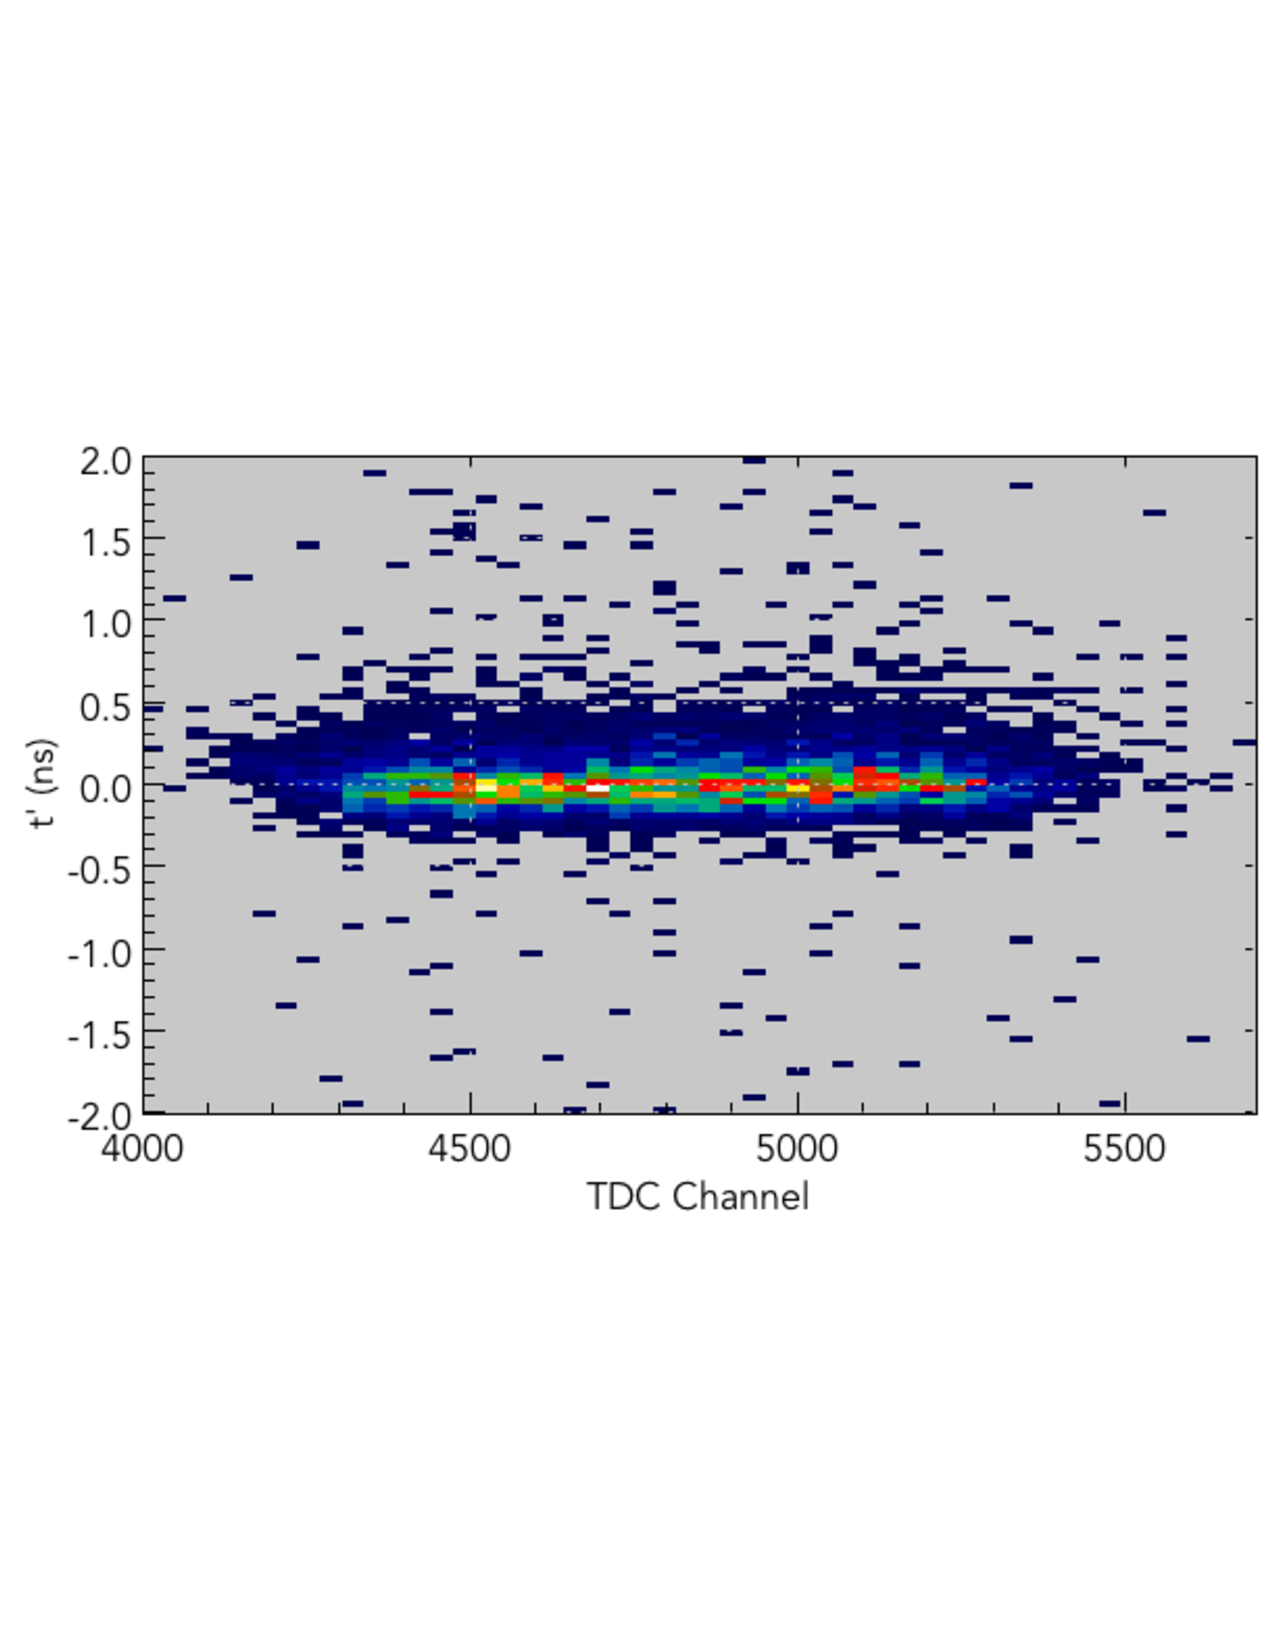
\includegraphics[width=0.38\textwidth,natwidth=610,natheight=642]{pics/tdc-plot.pdf}}}
\end{picture} 
\caption{Distribution of $t^{res}_L$ (ns) vs. TDC digitization bin for one representative left FTOF
panel-1b PMT. The TDC conversion constant for each input channel is that which forces the slope of
the linear fit to be zero.}
\label{tdc-plot}
\end{figure}
%%%%%%%%%%%%%%%%%%%%%%%%%%%%%%%%%%%%%%%%%%%%%%%%%%%%%%%%%%

\subsubsection{Counter Time Resolutions}
\label{tres-beam}

The effective time resolutions for each counter determined after complete calibrations of the FTOF
system are shown in Fig.~\ref{eff-tres}. These measurements are from a beam data run with 10.6-GeV
electrons incident on a 5-cm long liquid-hydrogen target. These time resolutions represents the current
quality of the overall CLAS12 calibrations. The results are based on calibration procedures that are not
yet fully optimized, as well as uncertainties in the reconstructed momentum and path length from the
forward track reconstruction. Note that the time resolution floor-term $\sigma_0$ discussed in
Section~\ref{res-sec} and Eq.(\ref{timing-func}) does not include the contributions from the
reconstructed path length uncertainties. These uncertainties are polar and azimuthal angle dependent.
Near the torus coils the true magnetic field has different variations than accounted for in our conductor
model used to generate the field for the event reconstruction. Furthermore, the path length uncertainties
grow strongly for high momentum tracks at small angles, which represent the dominant part of our kinematic
phase space at 10.6~GeV. It is also important to mention that studies of the CLAS12 subsystem detector
alignment based on survey data and based on zero-field straight track data are in progress. Misalignments
of the detector affect the quality and accuracy of the reconstruction. When all of these uncertainties and
misalignments are accounted for their contribution to the floor-term of the resolution function will be
reduced.

Nevertheless, the time resolutions already achieved reasonably meet the system design specifications in the
forward direction outlined in Section~\ref{sec:overview} and shown in Table~\ref{spec-table}. For the
panel-2 counters the time resolutions are 200-250~ps, but the calibrations are presently limited by statistics,
by the use of low-momentum protons in the calibration sample (as discussed in Section~\ref{beam-data-calib}),
and by the use of the low-resolution 100~ps LSB TDCs for readout. With these FTOF counter resolutions, the
quality of the particle identification in the Forward Detector of CLAS12 allows the experimental program in
Hall~B to reach its goals. As further operating experience with CLAS12 is gained, we expect to realize further
modest but important improvements in the FTOF time resolution that will allow $\pi/K$, $\pi/p$, and $K/p$
separation in the Forward Detector of CLAS12 to be pushed to higher momenta than currently seen.

%%%%%%%%%%%%%%%%%%%%%%%%%%%%%%%%%%%%%%%%%%%%%%%%%%%%%%%%%
\begin{figure}[htbp]
\vspace{1.1cm}
\begin{picture}(50,50) 
\put(-5,-45)
{\hbox{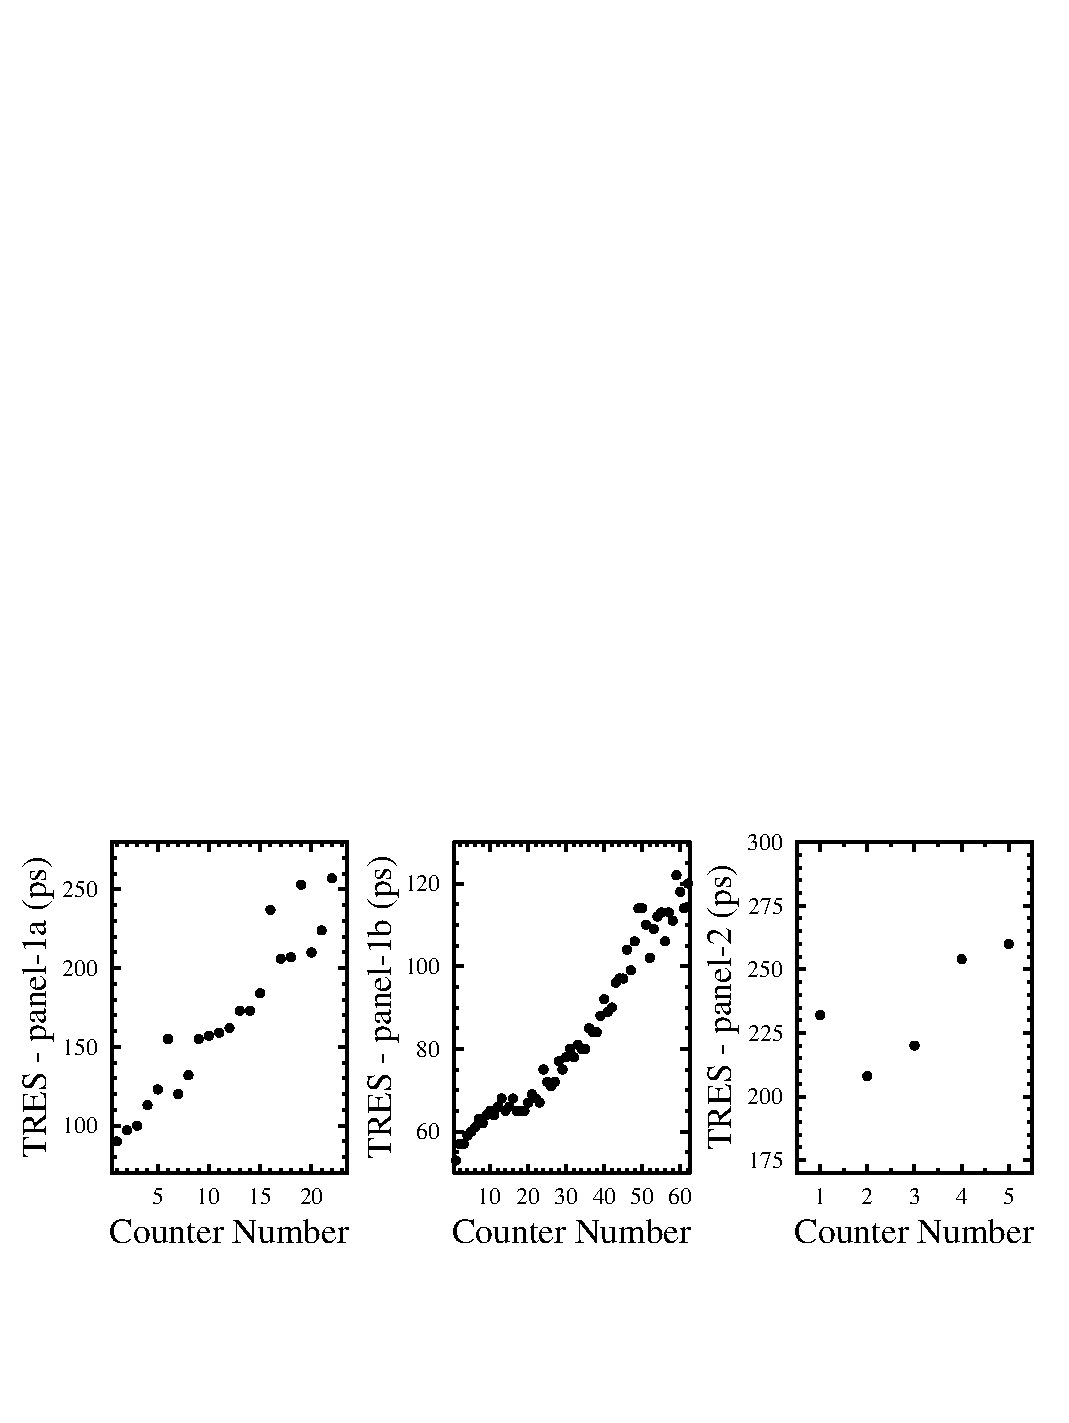
\includegraphics[width=0.59\textwidth,natwidth=610,natheight=642]{pics/res-r5038.pdf}}}
\end{picture} 
\caption{The measured effective time resolution (ps) vs. counter number for each of the FTOF counters
in sector~1 as determined using final state leptons and pions for panel-1a and panel-1b and pions and
protons for panel-2.}
\label{eff-tres}
\end{figure}
%%%%%%%%%%%%%%%%%%%%%%%%%%%%%%%%%%%%%%%%%%%%%%%%%%%%%%%%%

\subsubsection{Counter Hit Times}
\label{cluster}

After completion of each of the timing calibration steps discussed in this section, the FTOF hit time associated
with a matched charged particle track can be determined. Putting all of the timing corrections together, the
track hit time reconstructed from the readout of the left and right PMTs are given by:
\begin{multline}
t_{L,R} = (CONV \cdot TDC_{L,R}) - t_{L,R}^{walk} \\ \mp \frac{C_{LR}}{2} + C_{RF} + C_{p2p},
\end{multline}

\noindent
where $CONV$ is the TDC digitization bin to time conversion factor, $TDC$ is the measured TDC value
relative to the trigger signal, $t^{walk}$ is the time-walk correction (which includes both the
position-independent and position-dependent time-walk corrections described in Section~\ref{sec-tw}),
$C_{LR}$ is the time shift to center the TDC difference distribution relative to the track coordinate at zero,
and $C_{RF}$ and $C_{p2p}$ are the time shifts to align all of the counter times with respect to the RF and to
each other, respectively.

The actual hit time associated with the track has to be corrected for the propagation time of the light from
the track hit point on the counter to the PMT. The final reported track hit time is then the average of
the left and right corrected PMT time. Another aspect of the FTOF hit reconstruction is associated
with tracks that cross through multiple scintillation bars as they pass through the FTOF system. These are
referred to a hit clusters. If a track passes through both panel-1b and panel-1a, the hit time from panel-1a
can be evolved back to the panel-1b hit location and the time information can be combined to give a hit time
with improved precision. Full details on the FTOF reconstruction algorithms, including hit times, and the hit
clustering and matching algorithms are provided in Refs.~\cite{recon-nim,ftof-recon}.

\subsection{Beam Performance}  
\label{sec:beam}

The first in-beam characterization of the FTOF system took place during the Dec. 2017 to Feb. 2018
CLAS12 Engineering Run and subsequently during the first physics production running periods that took
place from Mar. - May 2018 and Sep. - Dec. 2018. During these periods the performance of the FTOF
system was tested at different beam energies (2.2, 6.5, 7.5, 10.6~GeV), different torus and solenoid
magnetic field strengths and polarities (from 0 field to full field for both magnets), and over a range of
beam-target luminosities up to the nominal planned CLAS12 luminosity of $1 \times 10^{35}$~cm$^{-2}$s$^{-1}$.
In this section the measured scaler rates and PMT currents as a function of beam current are presented, as
well as the reconstruction results and particle identification capabilities relative to the system specifications
based on the current system calibrations.

\subsubsection{FTOF Rates and PMT Currents}

The count rates during beam operations can be viewed during data taking using the scalers associated
with the discriminators or with the FADCs. The threshold applied for these scalers are set at 1~MeV.
During a beam current scan from 5~nA to 70~nA with a 10.6-GeV electron beam incident upon the 5-cm long
liquid-hydrogen target (where 75~nA corresponds roughly to the nominal CLAS12 design luminosity of
$1 \times 10^{35}$~cm$^{-2}$s$^{-1}$) the average count rate in the different FTOF counters was studied.
Averaged over the three different arrays, the results shown in Fig.~\ref{ftof-rates}, display a reasonably
linear behavior. The rates in panel-1a are about a factor of two larger than those for panel-1b. This is in
agreement with the fact that the panel-1a counters are 2.5 times wider than the panel-1b counters. However,
some portion of the incident radiation is absorbed in the panel-1b counters reducing the flux seen in panel-1a.
At the nominal luminosity of CLAS12, the average measured rates in the panel-1b counters are about 500~kHz
and those in panel-1a are about 1~MHz.

%%%%%%%%%%%%%%%%%%%%%%%%%%%%%%%%%%%%%%%%%%%%%%%%%%%%%%%%%
\begin{figure}[htbp]
\vspace{1.9cm}
\begin{picture}(50,50) 
\put(-5,-45)
{\hbox{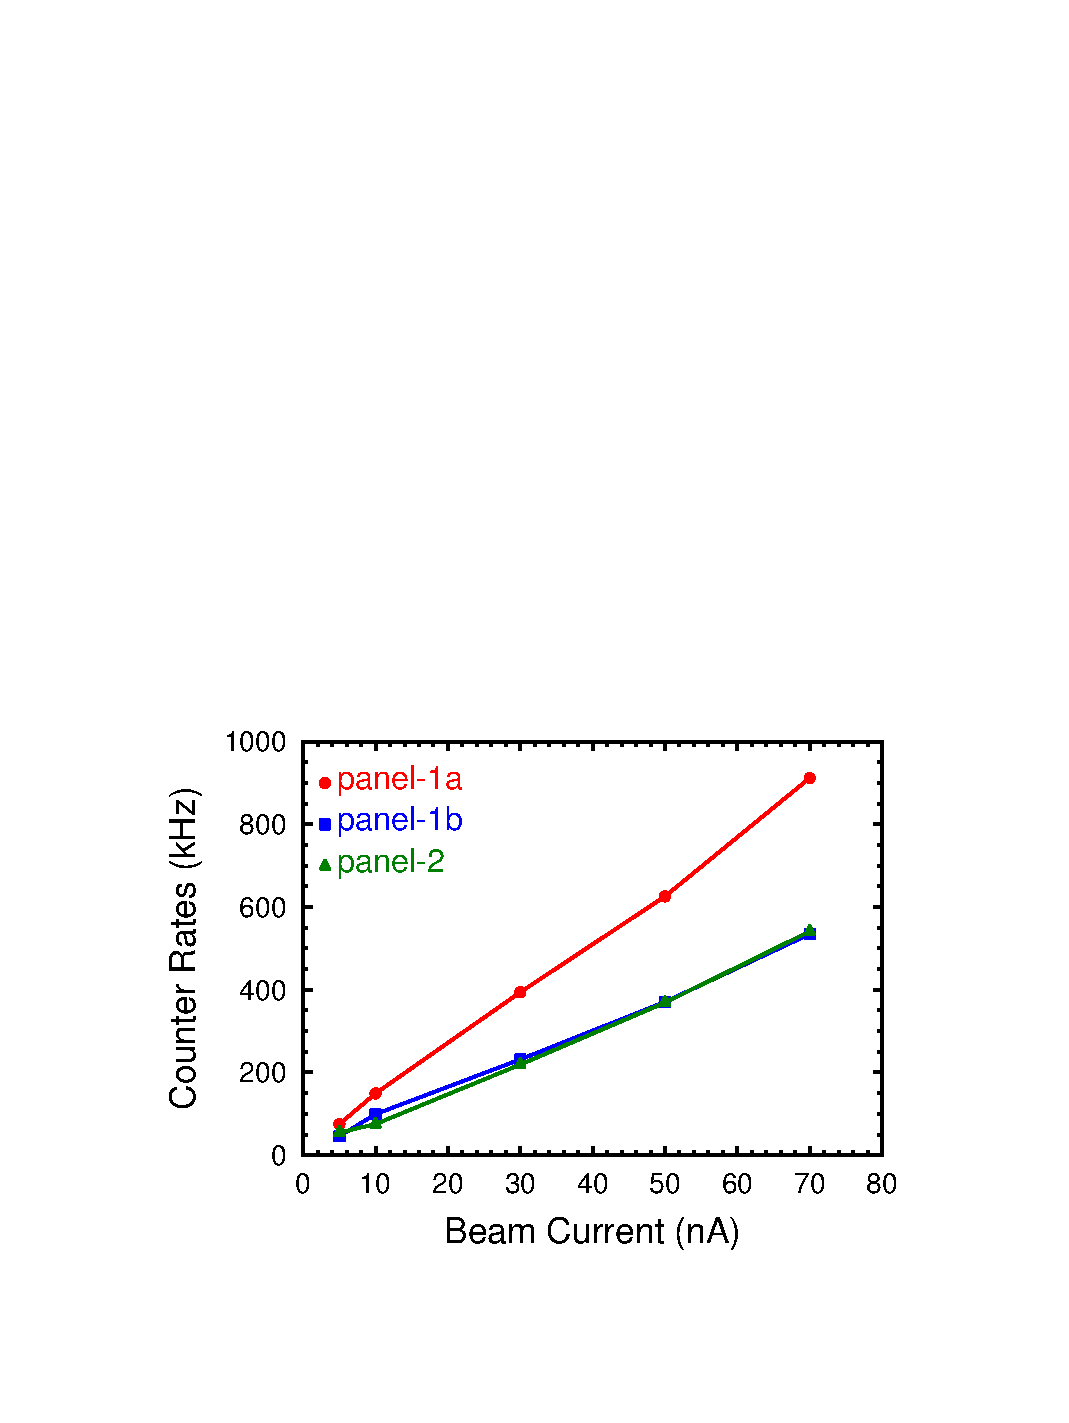
\includegraphics[width=0.6\textwidth,natwidth=610,natheight=642]{pics/ftof-rates.pdf}}}
\end{picture} 
\caption{Measured FTOF counter rates (kHz) for 10.6-GeV electrons on a liquid-hydrogen target as a
function of beam current (nA) employing hardware thresholds of approximately 1~MeV. The nominal
CLAS12 operating luminosity of $1 \times 10^{35}$ cm$^{-2}$s$^{-1}$ corresponds to a beam current
of $\sim$75~nA. The red circles correspond to the average panel-1a counter rates, the blue squares
to the average panel-1b counter rates, and the green triangles to the average panel-2 counter rates.}
\label{ftof-rates}
\end{figure}
%%%%%%%%%%%%%%%%%%%%%%%%%%%%%%%%%%%%%%%%%%%%%%%%%%%%%%%%%

Based on a detailed simulation of the full CLAS12 detector and beamline based on our GEANT-4 Monte
Carlo called GEMC~\cite{sim-nim}, the response of the FTOF with an 11~GeV electron beam incident upon
a 5-cm liquid-hydrogen target has been studied. Shown in Fig.~\ref{ftof-gemc} are the overall rates
associated with hits above the readout threshold, including contributions from photons, neutrons, and
charged particles. By far the dominant contribution to the overall measured FTOF rate is associated with
low energy photons, whose energy deposition in the counters is significantly less than the contribution from
minimum-ionizing hadrons. The results from Fig.~\ref{ftof-rates} (data) and Fig.~\ref{ftof-gemc} (Monte
Carlo) agree to within a factor of two. However, the measured rates depend very strongly on the hardware
thresholds. The threshold set for the FADC readout and on the discriminator are not set directly on the
deposited energy, but on signal pulse height in the case of the discriminators or on a digitized amplitude in
the FADC. The set threshold on the hardware mentioned in Section~\ref{sec-elec} are only approximately
set to 1~MeV.

%%%%%%%%%%%%%%%%%%%%%%%%%%%%%%%%%%%%%%%%%%%%%%%%%%%%%%%%%
\begin{figure}[htbp]
\vspace{2.1cm}
\begin{picture}(50,50) 
\put(-13,-52)
{\hbox{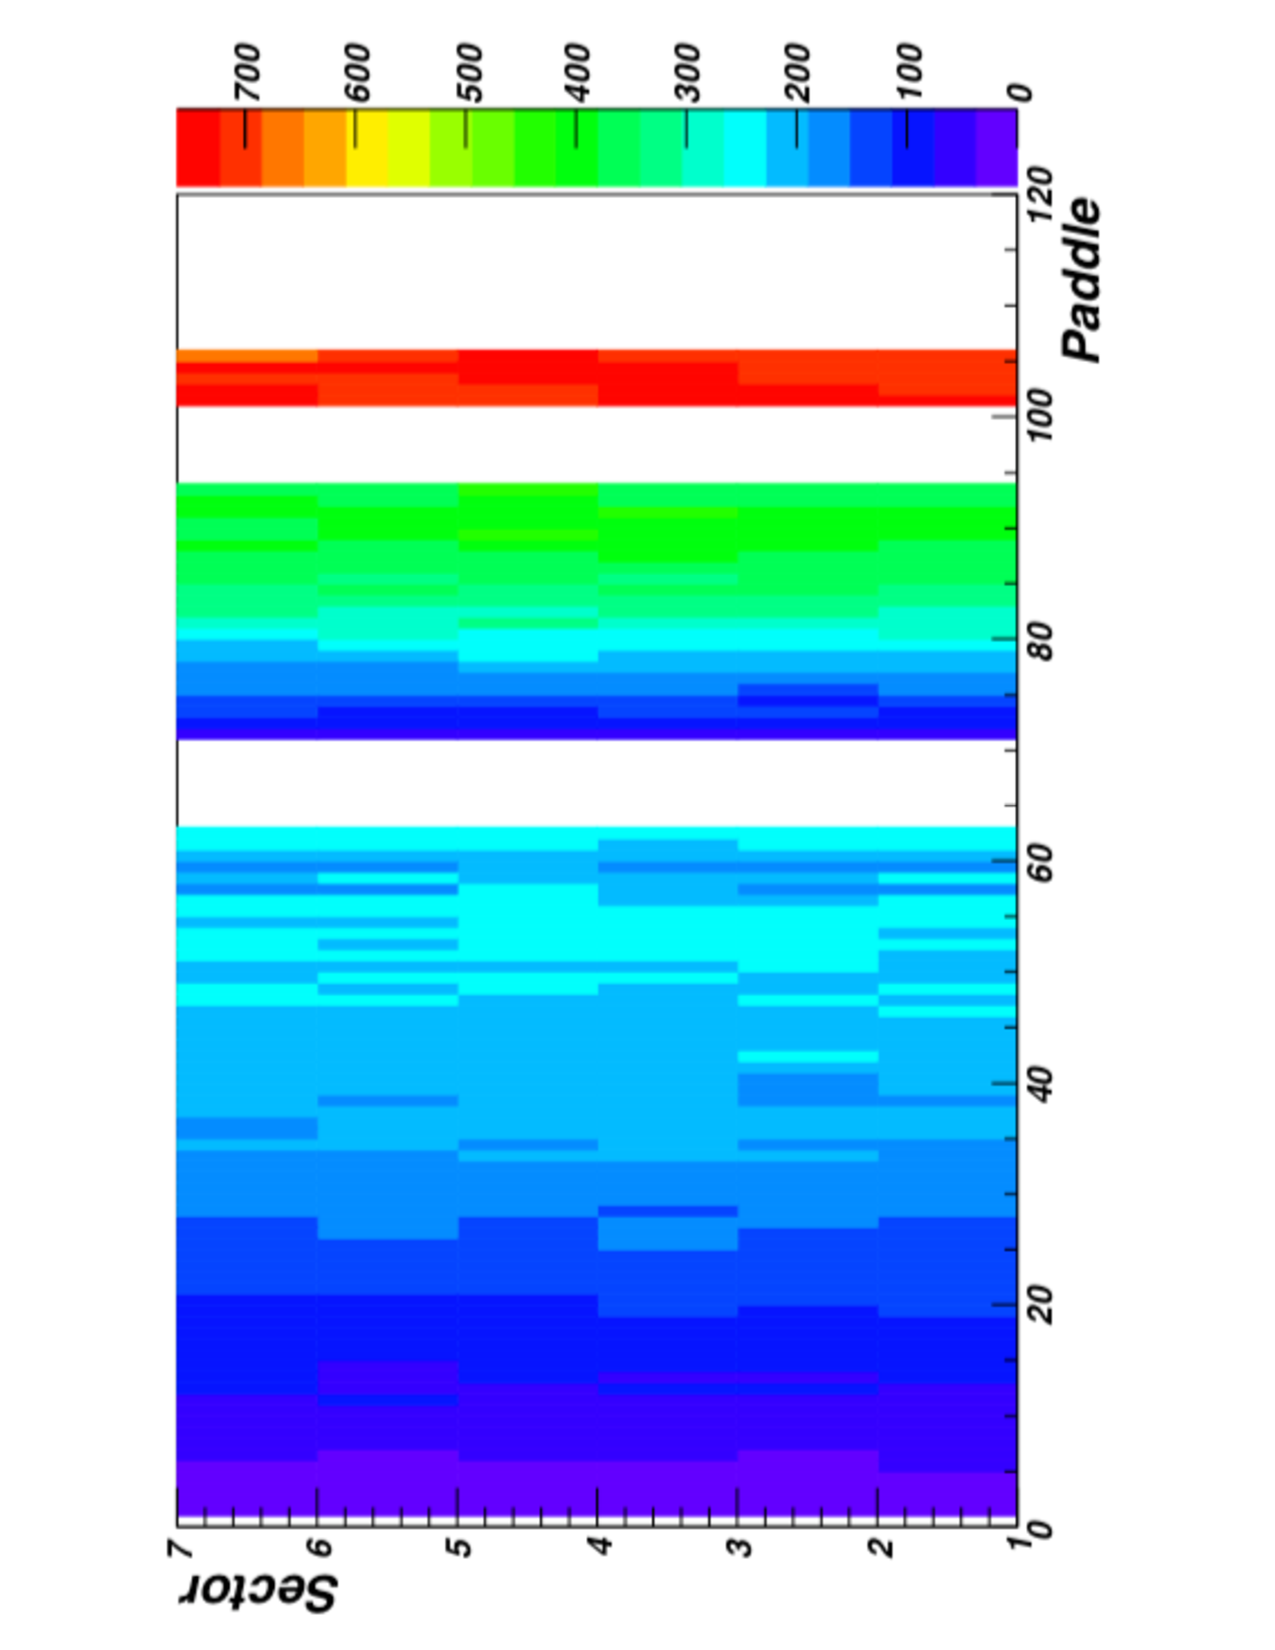
\includegraphics[width=0.43\textwidth,natwidth=610,natheight=642]{pics/mc-rates.pdf}}}
\end{picture} 
\caption{Simulation results for the FTOF counter rates (kHz) for each sector for 11~GeV electrons on
a liquid-hydrogen target at the nominal CLAS12 design luminosity of $1 \times 10^{35}$~cm$^{-2}$s$^{-1}$.
The rates are calculated for a 1-MeV deposited-energy threshold and expressed in kHz. Here the
left-most group of 62 paddles corresponds to panel-1b, the middle group of 23 paddles corresponds to
panel-1a, and the right-most group of 5 paddles corresponds to panel-2.}
\label{ftof-gemc}
\end{figure}
%%%%%%%%%%%%%%%%%%%%%%%%%%%%%%%%%%%%%%%%%%%%%%%%%%%%%%%%%

The average PMT current is directly proportional to the average number of photoelectrons
$\langle N_{pe} \rangle$ created at the photocathode by the scintillation light and the average incident
charged particle event rate $\langle R \rangle$. This current can be expressed as:

\begin{equation}
\langle i_{PMT} \rangle = \langle N_{pe} \rangle \cdot Q_e \cdot G \cdot \langle R \rangle,
\end{equation}

\noindent
where $Q_e = 1.6 \times 10^{-19}$ C/e is the electron charge and $G$ is the PMT gain (assumed to
be $1 \times 10^6$). Using the photoelectron statistics estimated in Section~\ref{res-sec},
Fig.~\ref{mc-pmt-currents} shows the predictions of the PMT anode currents for all of the FTOF
counters at nominal operating luminosity at 11~GeV from our detailed GEANT-4 Monte Carlo
studies~\cite{gemc-cn2017}. These predictions show typical PMT anode currents in the panel-1a and
panel-1b PMTs at the level of 5~$\mu$A to 10~$\mu$A increasing linearly with counter length. Direct
in-beam measurements of the PMT anode currents (made connecting a picoammeter to the PMT anode
output) are shown in Fig.~\ref{pmt-currents}. The in-beam measurements are in good accord with the
simulation expectations. Note that the measured anode currents reflect the current integrated over
all incident particles down to zero threshold. The comparison of data to Monte Carlo avoids the issues
with the threshold uncertainty mentioned above when comparing scaler rates between data and Monte
Carlo and serves to validate the Monte Carlo simulation and its modeling of the FTOF.

%%%%%%%%%%%%%%%%%%%%%%%%%%%%%%%%%%%%%%%%%%%%%%%%%%%%%%%%%
\begin{figure}[ht]
\vspace{2.1cm}
\begin{picture}(50,50) 
\put(-13,-53)
{\hbox{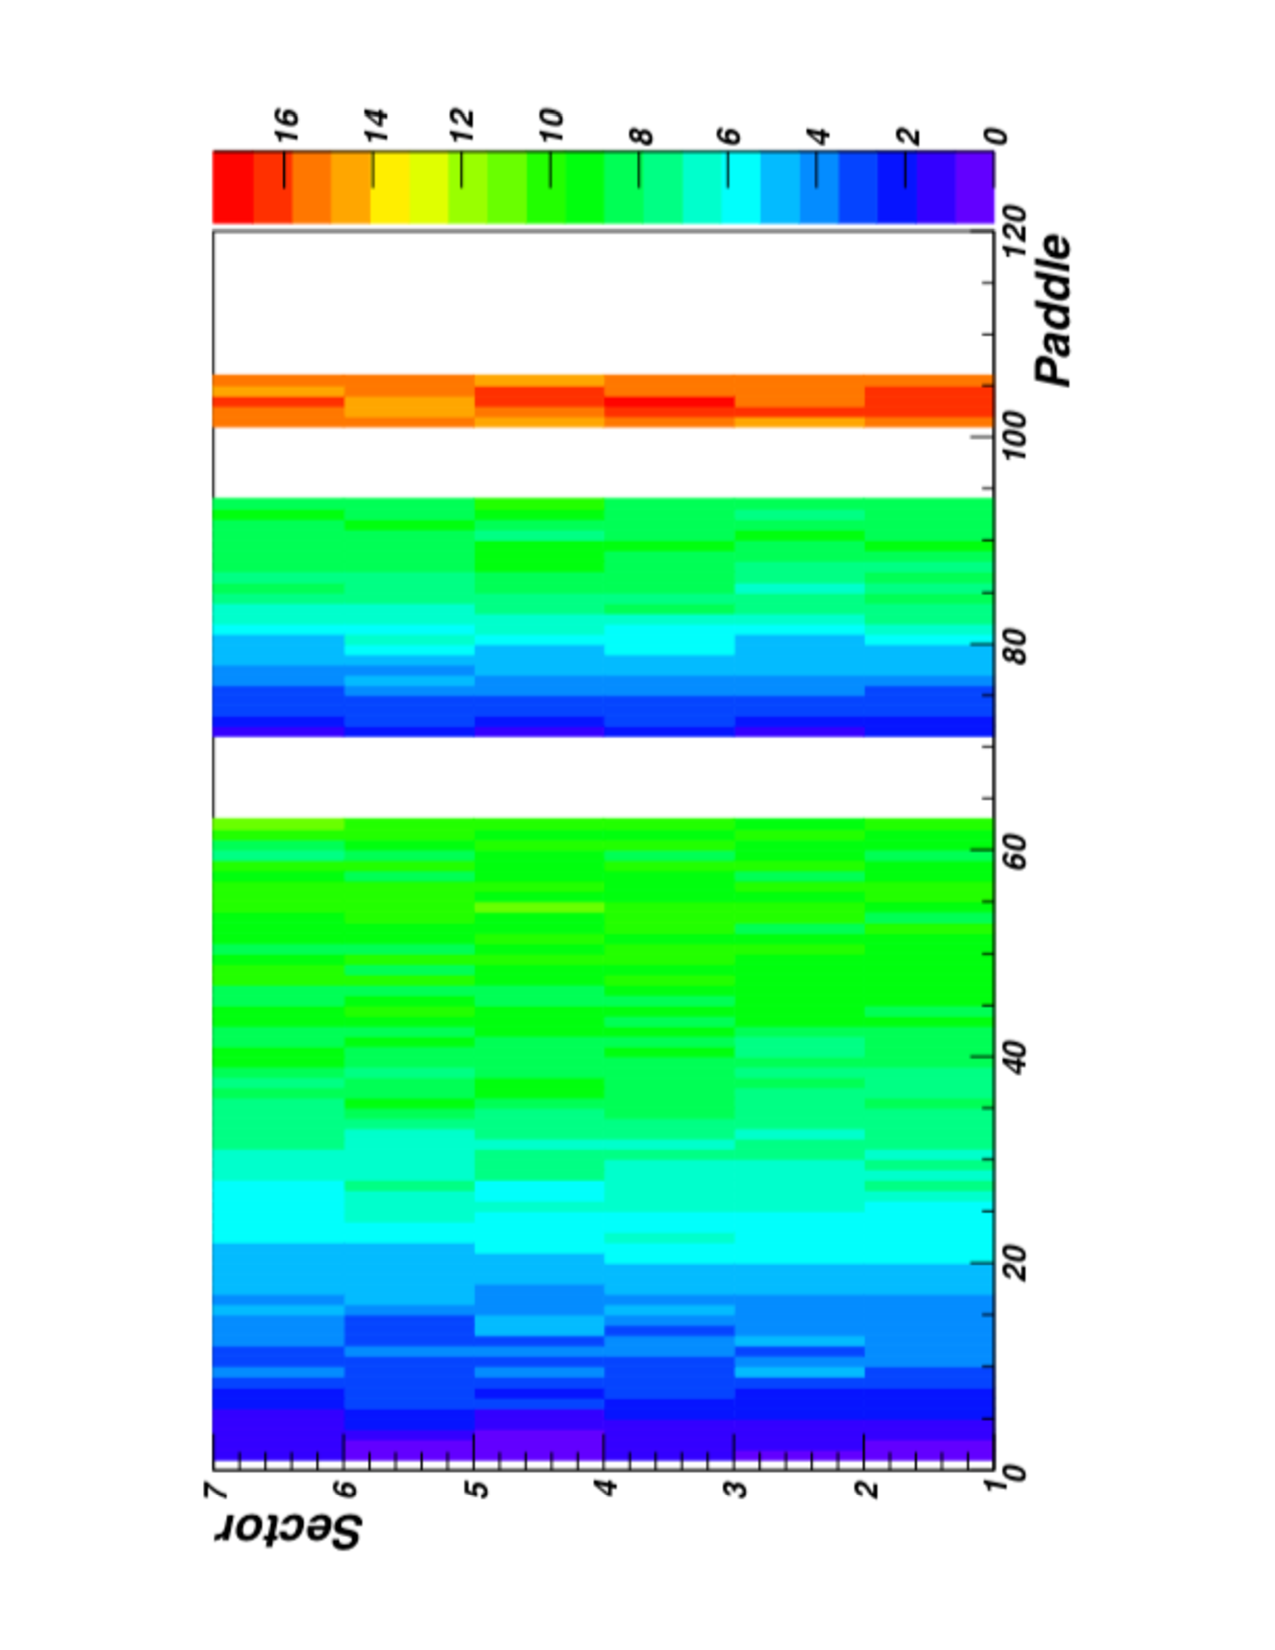
\includegraphics[width=0.43\textwidth,natwidth=610,natheight=642]{pics/mc-currents.pdf}}}
\end{picture} 
\caption{Computed PMT currents ($\mu$A) from Monte Carlo studies for each sector at the nominal
operating luminosity of CLAS12 of $1 \times 10^{35}$~cm$^{-2}$s$^{-1}$ with 11~GeV electrons
incident upon a liquid-hydrogen target. Here the left-most group of 62 paddles corresponds to
panel-1b, the middle group of 23 paddles corresponds to panel-1a, and the right-most group of 5
paddles corresponds to panel-2.}
\label{mc-pmt-currents}
\end{figure}
%%%%%%%%%%%%%%%%%%%%%%%%%%%%%%%%%%%%%%%%%%%%%%%%%%%%%%%%%

%%%%%%%%%%%%%%%%%%%%%%%%%%%%%%%%%%%%%%%%%%%%%%%%%%%%%%%%%
\begin{figure}[htbp]
\vspace{2.0cm}
\begin{picture}(50,50) 
\put(25,-50)
{\hbox{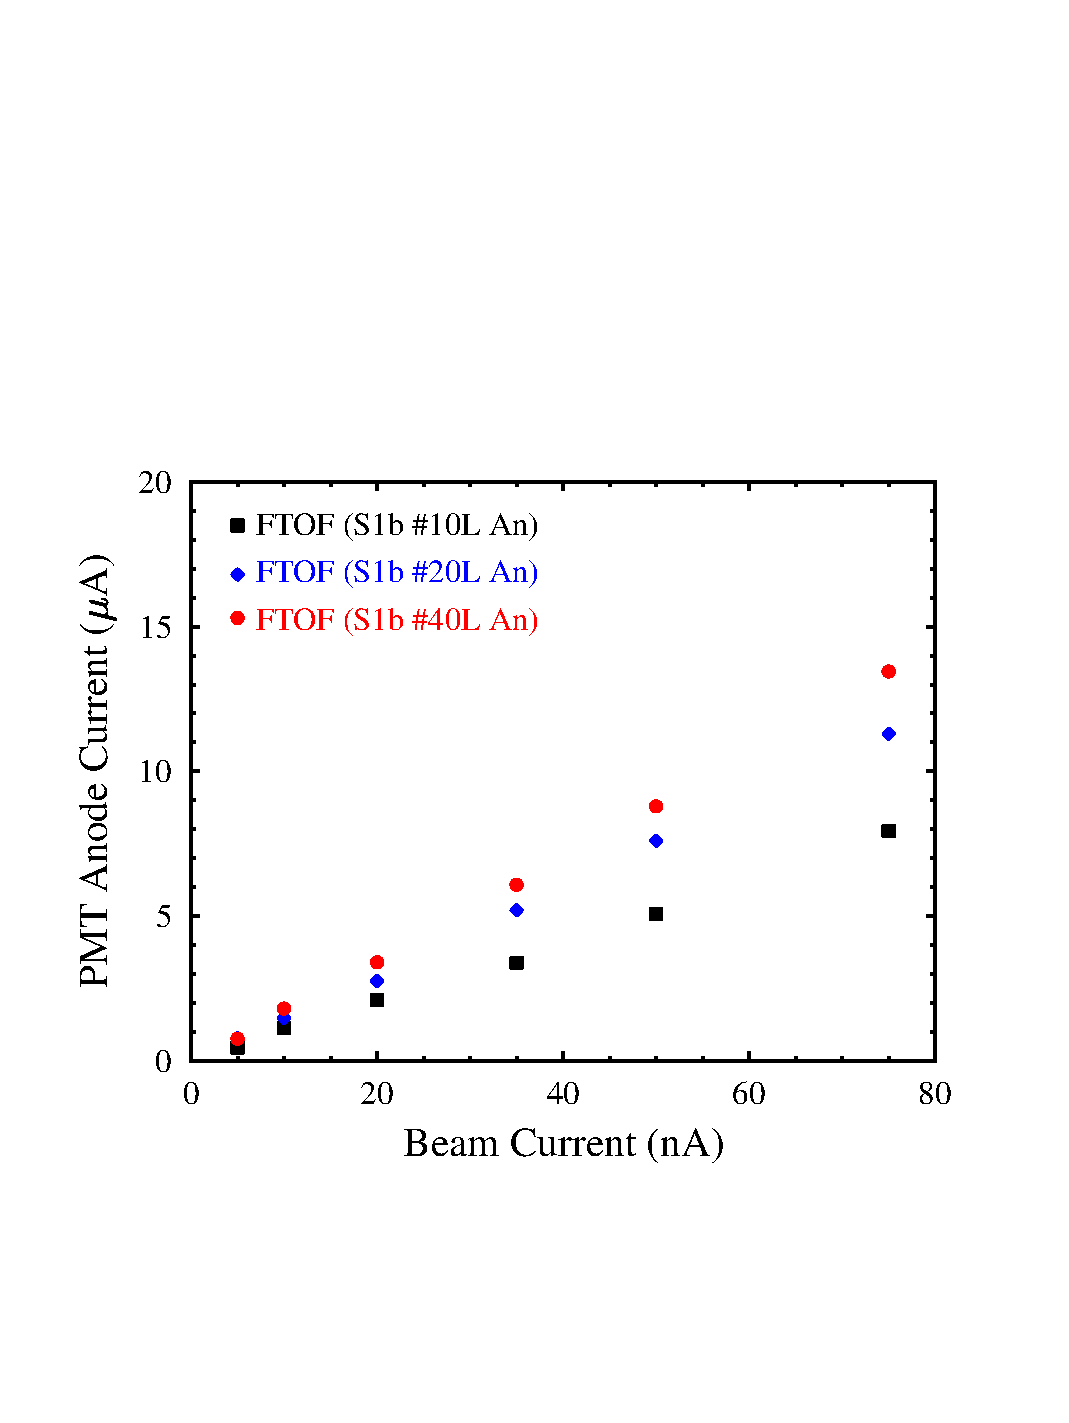
\includegraphics[width=0.45\textwidth,natwidth=610,natheight=642]{pics/full-ftof.pdf}}}
\end{picture} 
\caption{Measurements of the PMT anode current for representative panel-1b left-side PMTs
($N_C = 10, 20, 40$) as a function of beam current with a 10.6-GeV electron beam incident upon a
5-cm long liquid-hydrogen target.}
\label{pmt-currents}
\end{figure}
%%%%%%%%%%%%%%%%%%%%%%%%%%%%%%%%%%%%%%%%%%%%%%%%%%%%%%%%%

%%%%%%%%%%%%%%%%%%%%%%%%%%%%%%%%%%%%%%%%%%%%%%%%%%%%%%%%%
\begin{figure*}[htbp]
\vspace{3.1cm}
\begin{picture}(50,50) 
\put(-25,-140)
{\hbox{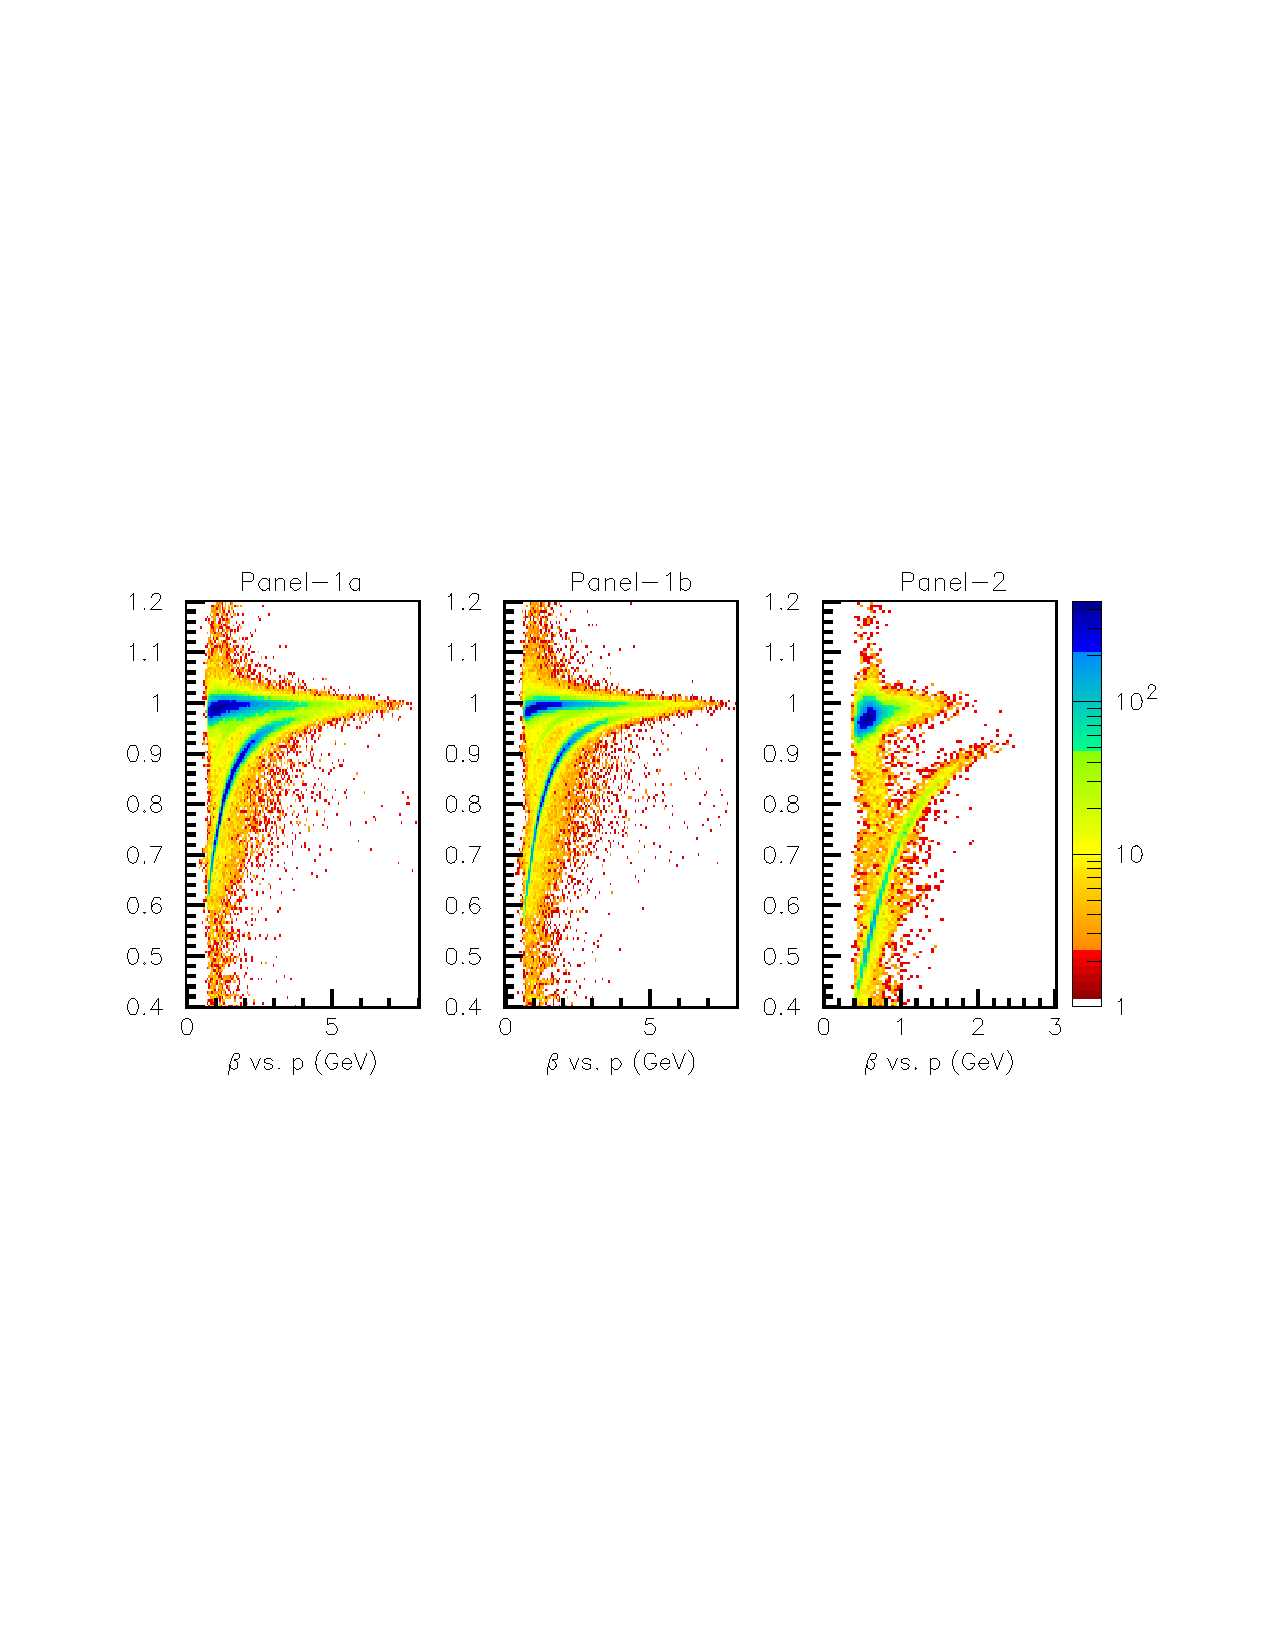
\includegraphics[width=0.93\textwidth,natwidth=610,natheight=642]{pics/bvsp.pdf}}}
\end{picture} 
\caption{Velocity of positive hadrons ($\beta$) versus momentum (GeV) for all counters in panel-1a (left),
panel-1b (middle), and panel-2 (right) from beam data with a 10.6~GeV electron beam incident on a
liquid-hydrogen target.}
\label{fig:betavsp}
\end{figure*}
%%%%%%%%%%%%%%%%%%%%%%%%%%%%%%%%%%%%%%%%%%%%%%%%%%%%%%%%%

\subsubsection{Reconstruction Results}

Particle identification in the Forward Detector of CLAS12 relies heavily on the combination of the
measured charged particle momentum from the forward tracking system and the flight time from
the target to the FTOF system. The vertex time is determined with respect to the accelerator RF,
modulo the RF period $T_{RF}$. The beam bunch for each event is identified using the flight time of
scattered electrons or high-momentum pions, traced back to the interaction point. The FTOF resolution
of $< 200$~ps allows clear selection of the correct RF beam bucket.

A plot of velocity versus momentum is shown in Fig.~\ref{fig:betavsp} for positively charged particles
for the data taken with a 10.6-GeV electron beam incident upon a 5-cm long liquid-hydrogen target.
These reconstructed beam data were based on initial calibrations of both the forward tracking system
and the FTOF. Here the distributions are presented separately for the counters in panel-1a, panel-1b,
and panel-2 summed over all CLAS12 Forward Detector sectors. Each distribution clearly shows primary
bands corresponding to $\pi^+$, $K^+$, and $p$ (see particle type labels on the panel-1b plot). These
distributions show evidence of other bands that correspond to so-called ``accidentals''. These are
mainly due to particles from neighboring RF beam buckets separated by $\pm n T_{RF}$, where $n$ is
an integer. These distributions demonstrate the particle separation limits for $\pi/K$, $\pi/p$, and $K/p$
vs. momentum.

To connect the current state of the particle identification limits from the FTOF system with those
detailed in Section~\ref{sec:overview}, Fig.~\ref{fig:masses} shows the reconstructed mass for positively
charged particles in the Forward Detector of CLAS12 based on initial calibrations of the FTOF system.
These plots are based only on the hit time reconstructed from the panel-1b counters. In order to avoid
timing resolution effects that would truncate the mass squared distribution when taking the square root,
Fig.~\ref{fig:masses} plots the reconstructed hadron mass squared using:

\begin{equation}
M^2 = p_p^2 \cdot \frac{1.-\beta^2}{\beta^2},~~~~\beta=\frac{P_L}{t_p c},
\end{equation}

\noindent
where $p_p$ is the particle momentum determined by the forward tracking system, $P_L$ is the hadron
path length from the event vertex in the target to the FTOF system, $t_p= \bar{t}_{hit} - t_{ST}$ is
the hadron flight time over $P_L$, and $c$ is the speed of light. Fig.~\ref{fig:masses} shows the mass
squared distributions for several bins in hadron momentum from 2~GeV to 5~GeV. Even with the current
state of CLAS12 detector calibrations, detector alignment, and knowledge of the torus and solenoid
magnetic field, these distributions show good separation between $\pi/K$ up to about 3~GeV and
separation of $\pi$ and $K$ from $p$ to about 5~GeV. Improvements in the FTOF and forward tracking
calibrations, detector alignment, and knowledge of the magnetic fields in the CLAS12 tracking volume
that are still expected should give improved particle identification and separation of the different charged
hadron species to higher momentum. In addition, employing the combined timing measurement for the hits in
panel-1a and panel-1b (see Section~\ref{cluster}) will also result in improved particle identification using the
FTOF system.

%%%%%%%%%%%%%%%%%%%%%%%%%%%%%%%%%%%%%%%%%%%%%%%%%%%%%%%%%
\begin{figure}[htbp]
\vspace{3.9cm}
\begin{picture}(50,50) 
\put(15,-65)
{\hbox{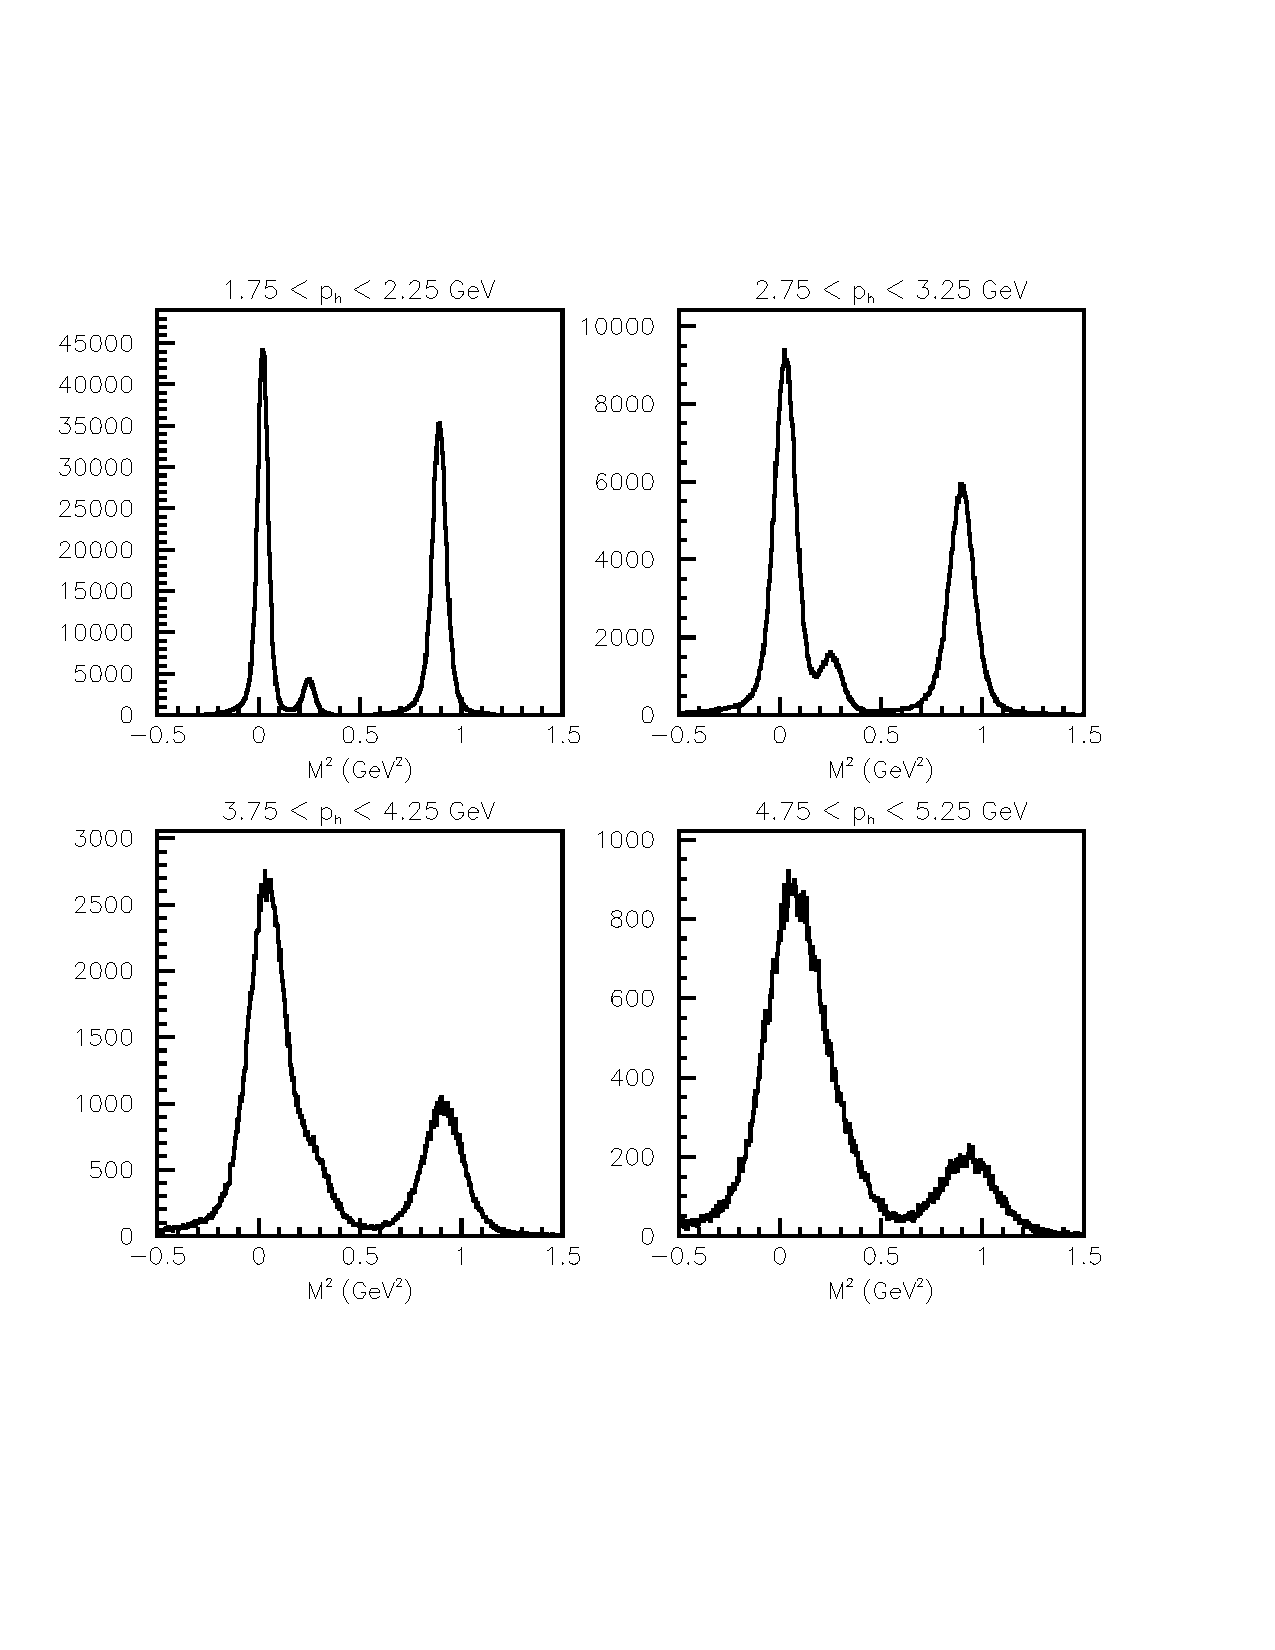
\includegraphics[width=0.45\textwidth,natwidth=610,natheight=642]{pics/massph.pdf}}}
\end{picture} 
\caption{Reconstructed mass squared (GeV$^2$) for positively charged particles from the timing in
the panel-1b FTOF counters from beam data with a 10.6-GeV electron beam incident on a liquid-hydrogen
target. The data are sorted into four bins in hadron momentum (UL) [1.75:2.25]~GeV, (UR) [2.75:3.25]~GeV,
(LL) [3.75:4.25]~GeV, and (LR) [4.75:5.25]~GeV and are based on the current CLAS12 detector calibrations,
detector alignments, and knowledge of the torus and solenoid field maps.}
\label{fig:masses}
\end{figure}
%%%%%%%%%%%%%%%%%%%%%%%%%%%%%%%%%%%%%%%%%%%%%%%%%%%%%%%%

\section{Summary}
\label{sec:summary}

We have designed and assembled a time-of-flight system for the Forward Detector of the new CLAS12
Spectrometer in Hall~B at Jefferson Lab known as the Forward Time-of-Flight or FTOF system, which
consists of 90 scintillation bars in each of the six sectors of the CLAS12 Forward Detector for a total of
540 counters. This design is based on rectangular counters varying in length from 17~cm to 426~cm in
three different counter arrays in each sector. In the polar angle range from 5$^\circ$ to 35$^\circ$ the
FTOF system consists of two layers of counters referred to as panel-1a and panel-1b. The panel-1a counters
were refurbished from the forward TOF counters that were part of the original CLAS spectrometer. The
panel-1b counters were newly constructed for CLAS12. Together the timing measurements from these
two arrays of counters currently provide effective time resolutions from 50~ps for the shortest counters at
small polar angles to 100~ps for the longest counters at large polar angles. In the polar angle range from
35$^\circ$ to 45$^\circ$ the FTOF system consists of the panel-2 counters that were refurbished from the
CLAS TOF system. These counters provide effective time resolutions of about 250~ps. With these time
resolutions the FTOF system can separate $\pi/K$ to 2.8~GeV, $K/p$ to 4.8~GeV, and $\pi/p$ to 5.4~GeV
with 4$\sigma$ separation with up to an order of magnitude difference in the relative yields. The specifications
are sufficient to meet the design particle identification requirements in the forward direction for the full
CLAS12 physics program. The performance of the FTOF system has been verified in extensive bench studies
in our cosmic ray test stands, as well as after installation in the first beam runs with the CLAS12 system in the
period from Dec. 2017 to Dec. 2018. 

\section*{Acknowledgments}

Many aspects in the development of the FTOF system benefited greatly from useful discussions with and
assistance from Sergey Boyarinov, Chris Cuevas, Haiyan Lu, Cole Smith, Elton Smith, and Veronique Ziegler. The
panel-1b counters were built and tested at the University of South Carolina with the help of Jesse Anderson,
Robert Steinman, Felician Stratman, Nick Tyler, and a dedicated team of graduate and undergraduate students.
We also thank the Hall~B technical crew for their efforts during counter installation and cabling, as well as
members of the Hall~B Engineering and Design Groups that contributed to the detector advancement during the
design stage. This material is based upon work supported by the U.S. Department of Energy, Office of Science,
Office of Nuclear Physics under contract DE-AC05-06OR23177 and was also supported by the National Science
Foundation grant PHY-1205782.

\begin{thebibliography}{99}

\bibitem{clas12-nim}
V.D. Burkert {\it et al.}, {\it ``The CLAS12 Spectrometer at Jefferson Laboratory''}, to be published in
Nucl. Inst. and Meth. A, (2020). (see this issue)
  
\bibitem{clas-nim}
B.A. Mecking {\it et al.}, Nucl. Inst. and Meth. {\bf A503}, 513 (2003).

\bibitem{dc-nim}
M.D. Mestayer {\it et al.}, {\it ``The CLAS12 Drift Chamber System''}, to be published in Nucl. Inst.
and Meth. A, (2020). (see this issue)

\bibitem{htcc-nim}
Y. Sharabian {\it et al.}, {\it ``The CLAS12 High Threshold Cherenkov Counter''}, to be published in Nucl. Inst.
and Meth. A, (2020). (see this issue)
  
\bibitem{ltcc-nim}
M. Ungaro {\it et al.}, {\it ``The CLAS12 Low Threshold Cherenkov Counter''}, to be published in Nucl. Inst.
and Meth. A, (2020). (see this issue)
  
\bibitem{rich-nim}
M. Contalbrigo {\it et al.}, {\it ``The CLAS12 Ring Imaging Cherenkov Detector''}, to be published in Nucl. Inst.
and Meth. A, (2020). (see this issue)

\bibitem{ec-nim}
G. Asryan {\it et al.}, {\it ``The CLAS12 Electromagnetic Calorimeter''}, to be published in Nucl. Inst.
and Meth. A, (2020). (see this issue)

\bibitem{trigger-nim}
B. Raydo {\it et al.}, {\it ``The CLAS12 Trigger System''}, to be published in Nucl. Inst. and Meth. A, (2020).
(see this issue)
  
\bibitem{tof-nim}
E.S. Smith {\it et al.}, Nucl. Inst. and Meth. {\bf A432}, 265 (1999).

\bibitem{recon-nim}
V. Ziegler {\it et al.}, {\it ``CLAS12 Event Reconstruction''}, to be published in Nucl. Inst.
and Meth. A, (2020). (see this issue)

\bibitem{nim-p1b}
R.W. Gothe {\it et al.}, {\it ``A New Time-of-Flight System for CLAS12''}, to be submitted to Nucl. Inst.
and Meth A, (2020).

\bibitem{ftof-geom}
D.S. Carman, {\it ``Forward Time-of-Flight Geometry for CLAS12''}, CLAS12-Note 2014-005, (2014). \\
https://misportal.jlab.org/mis/physics/clas12/\\ viewFile.cfm/2014-005.pdf?documentId=13

\bibitem{daq-nim}
S. Boyarinov {\it et al.}, {\it ``The CLAS12 Data Acquisition System''}, to be published in Nucl. Inst. and
Meth. A, (2020). (see this issue)

\bibitem{kuhlen}
M. Kuhlen, M. Moszynski, R. Stroynowski, E. Wicklund, and B. Milliken, Nucl.  Instr. and Meth.
{\bf A301}, 223 (1991).

\bibitem{scint-mat-ref}
https://www.crystals.saint-gobain.com/sites/imdf.crystals.com/\\
files/documents/bc400-404-408-412-416-data-sheet.pdf

\bibitem{ftof-shields}
D.S. Carman and V. Baturin, {\it ``CLAS12 FTOF Studies: Rate and Magnetic Shielding Effects on PMT Timing
Resolutions''}, CLAS-Note 2011-018, (2011).\\
https://misportal.jlab.org/ul/Physics/Hall-B/clas/viewFile.cfm/2011-018.pdf?documentId=653

\bibitem{fadc-manual}
JLab 250~MHz FADC manual, https://www.jlab.org/\\ Hall-B/ftof/manuals/FADC250UsersManual.pdf
  
\bibitem{epics}
EPICS (Experimental Physics and Industrial Control System),\\ http://www.aps.anl.gov/epics

\bibitem{dsc-cn2013-001}
D.S. Carman, {\it ``CLAS12 FTOF Panel-1a and Panel-2 Refurbishment and Baseline Test Results''},
CLAS12-Note 2013-001, (2013).\\
https://misportal.jlab.org/mis/physics/clas12/\\ viewFile.cfm/2013-001.pdf?documentId=1

\bibitem{Gi86} 
R.T. Giles, F.M. Pipkin, and J.P. Wolinski, Nucl. Instr. and Meth. A {\bf 252}, 41 (1986).

\bibitem{kajino}
T. Yamaoka, F. Kajino, I. Tada, S. Hayashi, {\it ``Absolute Number Calibration of Photoelectrons of
Photomultiplier Tubes Using the Nature of Statistical Distribution''}, Proceedings of the 28th International
Cosmic Ray Conference, July 31 - August 7, 2003, editors: T. Kajita, Y. Asaoka, A. Kawachi, Y. Matsubara, and
M. Sasaki, p. 2871 (2003).

\bibitem{pmt-currents}
D.S. Carman, {\it ``Forward Time-of-Flight PMT Currents''}, FTOF internal note, 
https://www.jlab.org/Hall-B/ftof/notes/ftof\_currents.pdf

\bibitem{ftof-calib}
D.S. Carman, {\it ``Description of the Calibration Algorithms for the CLAS12 Forward Time-of-Flight System''},
FTOF internal note, \\
https://www.jlab.org/Hall-B/ftof/notes/ftof\_calib.pdf

\bibitem{ftof-recon}
D.S. Carman, {\it ``Forward Time-of-Flight Reconstruction for CLAS12''}, FTOF internal note, 
https://www.jlab.org/Hall-B/ftof/notes/ftof-recon.pdf

\bibitem{sim-nim}
M. Ungaro {\it et al.}, {\it ``The CLAS12 Geant4 Simulation''}, to be published in Nucl. Inst.
and Meth. A, (2020). (see this issue)

\bibitem{gemc-cn2017}
R. De Vita, D.S. Carman, C. Smith, S. Stepanyan, and M. Ungaro, {\it ``Study of the Electromagnetic Background
Rates in CLAS12''}, CLAS12-Note 2017-016, (2017).\\
https://misportal.jlab.org/mis/physics/clas12/\\ viewFile.cfm/2017-016.pdf?documentId=52

\end{thebibliography}

\end{document}
